\documentclass[11pt]{article}
\usepackage[margin=2cm]{geometry}
\usepackage{amsmath,amssymb}
\usepackage{graphicx}
\usepackage{booktabs}
\usepackage{array}
\usepackage{xcolor}
\usepackage[breakable]{tcolorbox}
\usepackage{enumitem}
\usepackage[hidelinks]{hyperref}
\allowdisplaybreaks
\setlength{\parindent}{0pt}
\setlength{\parskip}{4pt}
\definecolor{stepc}{HTML}{1F4E9E}
\definecolor{ansc}{HTML}{0B6E4F}
\newcommand{\solstep}[2]{\par\medskip{\color{stepc}\textbf{Step #1 --- #2}}\par\nopagebreak}
\newtcolorbox{probbox}[1]{colback=white,colframe=black!55,fonttitle=\bfseries,title={#1}}
\newtcolorbox{ansbox}{breakable,colback=ansc!6,colframe=ansc,fonttitle=\bfseries,title={Answer}}
\newtcolorbox{cardbox}[1]{breakable,colback=stepc!4,colframe=stepc,fonttitle=\bfseries,title={#1}}
\graphicspath{{../../../output/lecture5/5D_small_signal/}}
\title{Set 5D: MOSFET Amplifiers --- Small-Signal Analysis}
\author{ECEN 325 --- Lecture 5 (MOS Field-Effect Transistors) practice set}
\date{}
\begin{document}
\maketitle

\textbf{What this set trains.} The small-signal transfer function of single- and multi-stage MOSFET amplifiers with
the node-impedance method: $g_m$ of every transistor, the node impedances ($Z_{gate} = Z_{drain} = \infty$,
$Z_{source} = 1/g_m$), and the product of the node-to-node gains along the signal path. Then the Bode plot and the
steady-state output. $r_o = \infty$; capacitors marked $\infty$ are shorts at the signal frequencies. The DC drain
currents are given (they follow from a DC analysis as in sets 5A/5B). Problems 1--6 are easy, 7--12 medium, 13--18
hard. Try each problem before looking at its solution.


\begin{cardbox}{The Lecture-5 pipeline (use it for every problem in this lecture)}
\textbf{Tools --- this is all the theory you need (plus the Lecture-1--4 tools):}
\begin{enumerate}[label=\textbf{T\arabic*},leftmargin=2.2em,itemsep=1pt]
\item \emph{Square law} ($I_G = 0$ always). NMOS: $V_{ov} = V_{GS} - V_{tn}$; PMOS: $V_{ov} = V_{SG} - |V_{tp}|$.
      Cutoff if $V_{ov}\le 0$; active (saturation) if $|V_{DS}| \ge V_{ov}$:
      $I_D = \frac{k'}{2}\frac{W}{L}V_{ov}^2$; otherwise triode.
      A diode-connected transistor (gate tied to drain) is always active.
\item \emph{One quadratic per transistor:} with the gate voltage known, KVL gate $\to$ source $\to$ resistor $\to$
      known node gives $V_{known} = V_{GS} + R\,I_D$ with $I_D = \frac{k}{2}(V_{GS}-V_t)^2$. Of the two roots keep
      the one with $V_{GS} > V_t$.
\item \emph{Current mirror:} transistors with the same gate node and the same source node have the same $V_{GS}$,
      so their currents scale with $W/L$: $\frac{I_{D2}}{I_{D1}} = \frac{(W/L)_2}{(W/L)_1}$.
\item \emph{Small signal} ($r_o = \infty$): $g_m = k'\frac{W}{L}V_{ov} = \sqrt{2k'\frac{W}{L}I_D} = \frac{2I_D}{V_{ov}}$.
      Node impedances: $Z_{gate} = \infty$, $Z_{drain} = \infty$, $Z_{source} = \frac{1}{g_m}$. Gains: CS
      $\frac{v_d}{v_g} = -\frac{Z_D}{1/g_m + Z_S}$, CD $\frac{v_s}{v_g} = \frac{Z_S}{1/g_m + Z_S}$, CG
      $\frac{v_d}{v_s} = \frac{Z_D}{1/g_m}$ ($Z_D$, $Z_S$: everything else hanging on that node). For AC, DC supplies
      are ground and ``$\infty$'' capacitors are shorts.
\item \emph{Thevenin:} a linear network seen from two terminals is a source $V_{th}$ (its open-circuit voltage) in
      series with $R_{th}$ (its resistance with all sources set to zero). Branches $(V_k, R_k)$ in parallel combine to
      $V_{th} = \frac{\sum V_k/R_k}{\sum 1/R_k}$, $R_{th} = R_1\|R_2\|\dots$; a series resistor adds to $R_{th}$.
\end{enumerate}
\textbf{Steps:}
\begin{enumerate}[leftmargin=2.2em,itemsep=1pt]
\item \emph{DC:} assume every transistor active; gate voltages from dividers ($I_G=0$); one quadratic (or a mirror
      ratio) per transistor; then node voltages by KCL; \emph{verify} $V_{ov} > 0$ and $|V_{DS}| \ge V_{ov}$.
\item \emph{AC:} $g_m$ of every transistor; node impedances; multiply the node-to-node gains along the signal path;
      then standard form, Bode plot and output as in Lecture 1.
\item \emph{Design:} run the same relations backwards with the stated design rules, then check by analysis.
\end{enumerate}
\end{cardbox}

\section*{Problems}
\subsection*{Easy problems}
\begin{probbox}{Problem 5D.1 \hfill Easy}
For the amplifier below, find the small-signal transfer function $H(s)=\dfrac{V_o(s)}{V_i(s)}$ and sketch its magnitude Bode plot. Also find the steady-state output $V_o(t)$ for $V_i(t) = 0.01\sin\left(2\pi\cdot 100\,t\right)$. Assume $k'_n\frac{W}{L} = 1.1\,\mathrm{m}\mathrm{A/V^2}$, $V_{tn} = 1.4$\,V, $r_o = \infty$; the DC drain currents are $I_{D1} = 726\,\mu \mathrm{A}$.
\begin{center}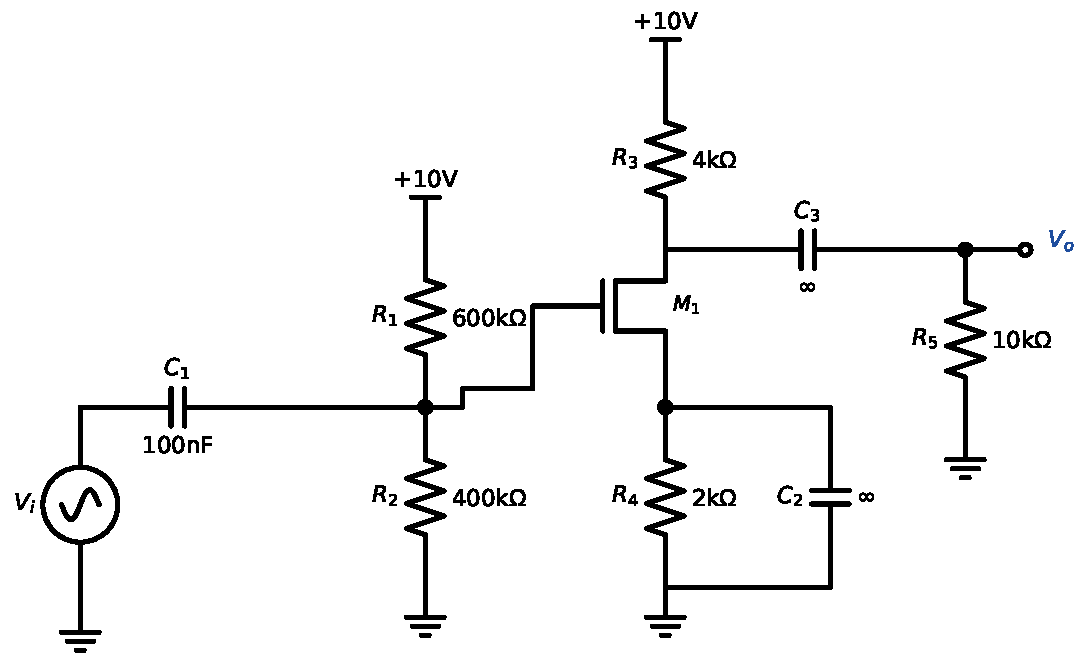
\includegraphics[width=\linewidth,height=7cm,keepaspectratio]{p01_circuit}\end{center}
\end{probbox}

\begin{probbox}{Problem 5D.2 \hfill Easy}
For the amplifier below, find the small-signal transfer function $H(s)=\dfrac{V_o(s)}{V_i(s)}$ and sketch its magnitude Bode plot. Also find the steady-state output $V_o(t)$ for $V_i(t) = 0.02\sin\left(2\pi\cdot 1000\,t\right)$. Assume $k'_p\frac{W}{L} = 850\,\mu \mathrm{A/V^2}$, $V_{tp} = -1.3$\,V, $r_o = \infty$; the DC drain currents are $I_{D1} = 378\,\mu \mathrm{A}$.
\begin{center}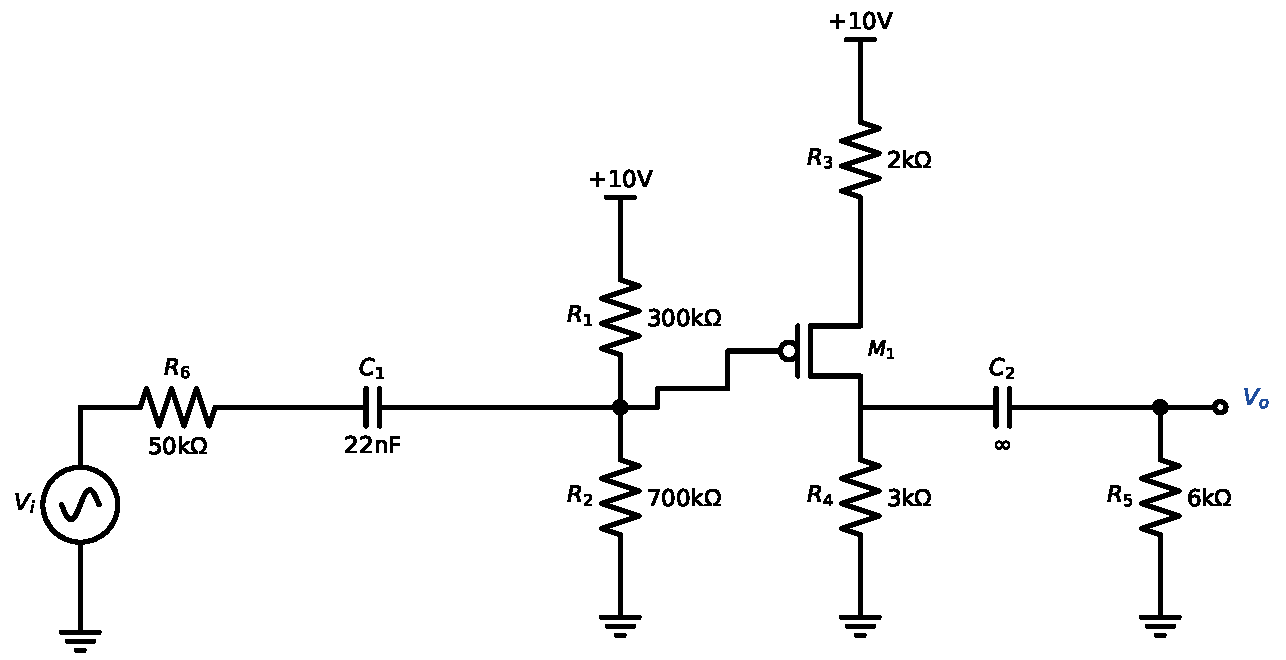
\includegraphics[width=\linewidth,height=7cm,keepaspectratio]{p02_circuit}\end{center}
\end{probbox}

\begin{probbox}{Problem 5D.3 \hfill Easy}
For the amplifier below, find the small-signal transfer function $H(s)=\dfrac{V_o(s)}{V_i(s)}$ and sketch its magnitude Bode plot. Also find the steady-state output $V_o(t)$ for $V_i(t) = 0.5\sin\left(2\pi\cdot 50\,t\right)$. Assume $k'_n\frac{W}{L} = 1.1\,\mathrm{m}\mathrm{A/V^2}$, $V_{tn} = 1.4$\,V, $r_o = \infty$; the DC drain currents are $I_{D1} = 1.37\,\mathrm{m}\mathrm{A}$.
\begin{center}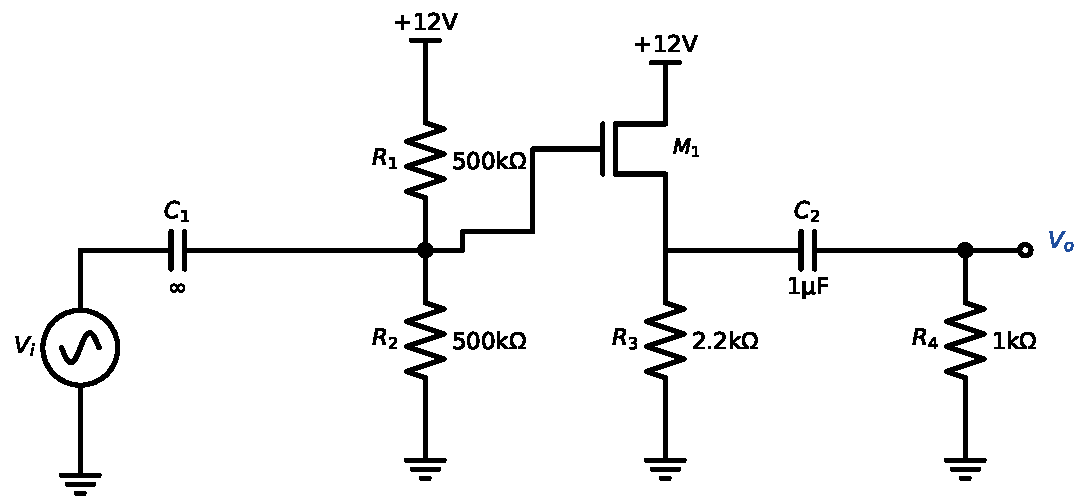
\includegraphics[width=\linewidth,height=7cm,keepaspectratio]{p03_circuit}\end{center}
\end{probbox}

\begin{probbox}{Problem 5D.4 \hfill Easy}
For the amplifier below, find the small-signal transfer function $H(s)=\dfrac{V_o(s)}{V_i(s)}$ and sketch its magnitude Bode plot. Also find the steady-state output $V_o(t)$ for $V_i(t) = 0.005\sin\left(2\pi\cdot 200\,t\right)$. Assume $k'_n\frac{W}{L} = 2\,\mathrm{m}\mathrm{A/V^2}$, $V_{tn} = 1$\,V, $r_o = \infty$; the DC drain currents are $I_{D1} = 444\,\mu \mathrm{A}$.
\begin{center}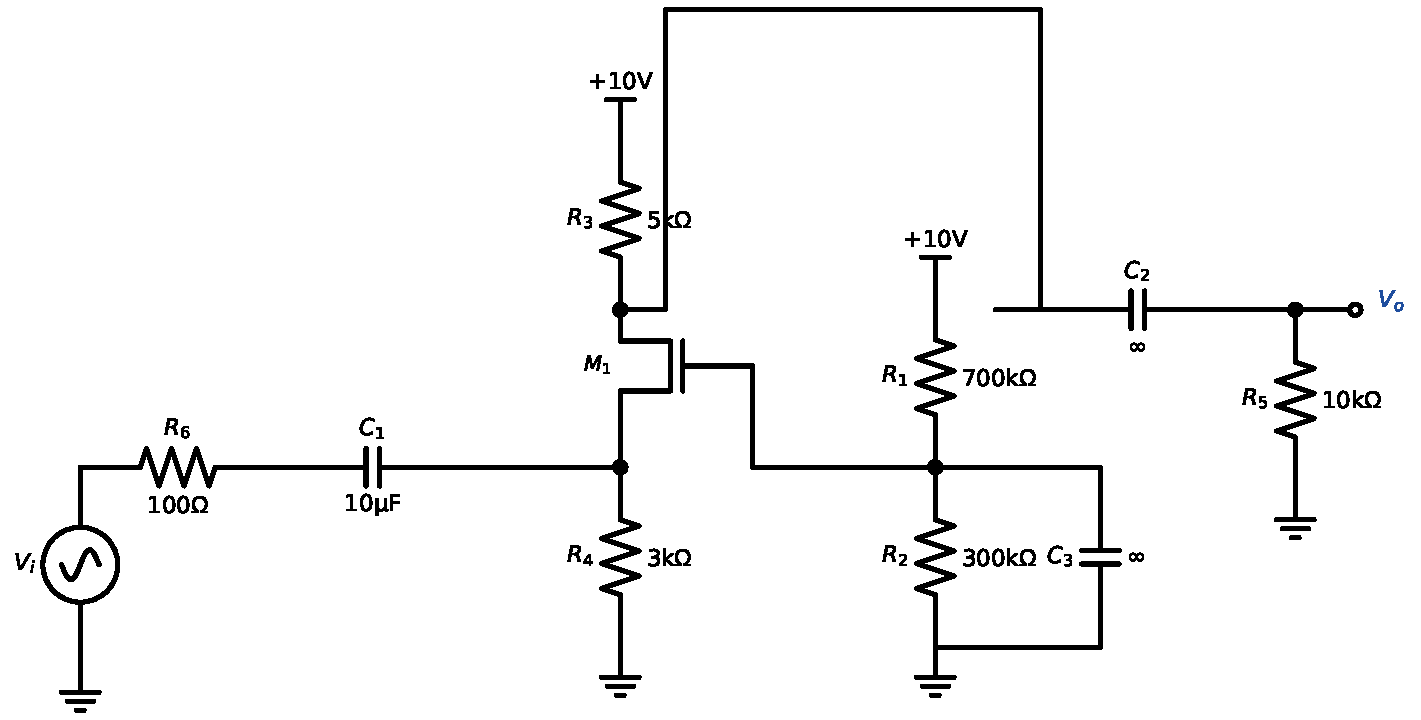
\includegraphics[width=\linewidth,height=7cm,keepaspectratio]{p04_circuit}\end{center}
\end{probbox}

\begin{probbox}{Problem 5D.5 \hfill Easy}
For the amplifier below, find the small-signal transfer function $H(s)=\dfrac{V_o(s)}{V_i(s)}$ and sketch its magnitude Bode plot. Also find the steady-state output $V_o(t)$ for $V_i(t) = 0.01\sin\left(2\pi\cdot 20000\,t\right)$. Assume $k'_n\frac{W}{L} = 2\,\mathrm{m}\mathrm{A/V^2}$, $V_{tn} = 1$\,V, $r_o = \infty$; the DC drain currents are $I_{D1} = 640\,\mu \mathrm{A}$.
\begin{center}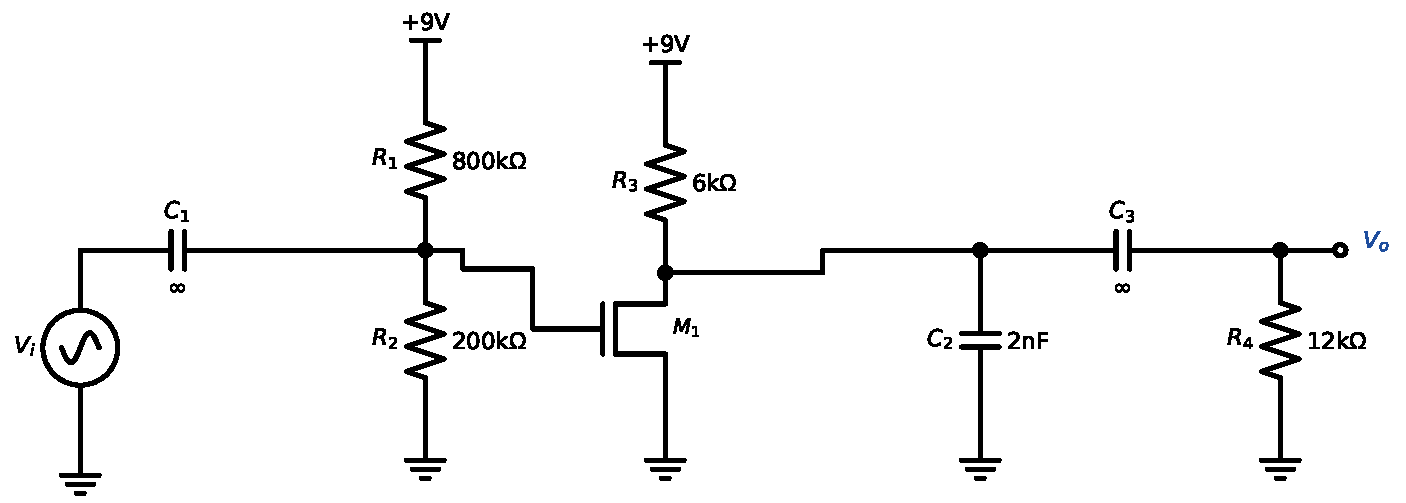
\includegraphics[width=\linewidth,height=7cm,keepaspectratio]{p05_circuit}\end{center}
\end{probbox}

\begin{probbox}{Problem 5D.6 \hfill Easy}
For the amplifier below, find the small-signal transfer function $H(s)=\dfrac{V_o(s)}{V_i(s)}$ and sketch its magnitude Bode plot. Also find the steady-state output $V_o(t)$ for $V_i(t) = 0.2\sin\left(2\pi\cdot 5\,t\right)$. Assume $k'_p\frac{W}{L} = 850\,\mu \mathrm{A/V^2}$, $V_{tp} = -1.3$\,V, $r_o = \infty$; the DC drain currents are $I_{D1} = 528\,\mu \mathrm{A}$.
\begin{center}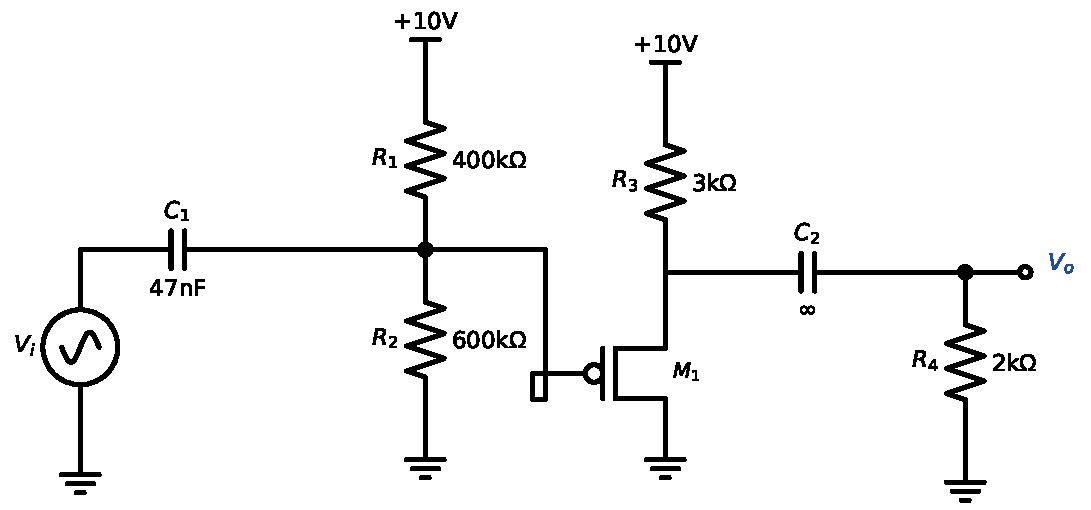
\includegraphics[width=\linewidth,height=7cm,keepaspectratio]{p06_circuit}\end{center}
\end{probbox}

\subsection*{Medium problems}
\begin{probbox}{Problem 5D.7 \hfill Medium}
For the amplifier below, find the small-signal transfer function $H(s)=\dfrac{V_o(s)}{V_i(s)}$ and sketch its magnitude Bode plot. Also find the steady-state output $V_o(t)$ for $V_i(t) = 0.005\sin\left(2\pi\cdot 10\,t\right)$. Assume $k'_n\frac{W}{L} = 1.1\,\mathrm{m}\mathrm{A/V^2}$, $V_{tn} = 1.4$\,V, $r_o = \infty$; the DC drain currents are $I_{D1} = 383\,\mu \mathrm{A}$, $I_{D2} = 626\,\mu \mathrm{A}$.
\begin{center}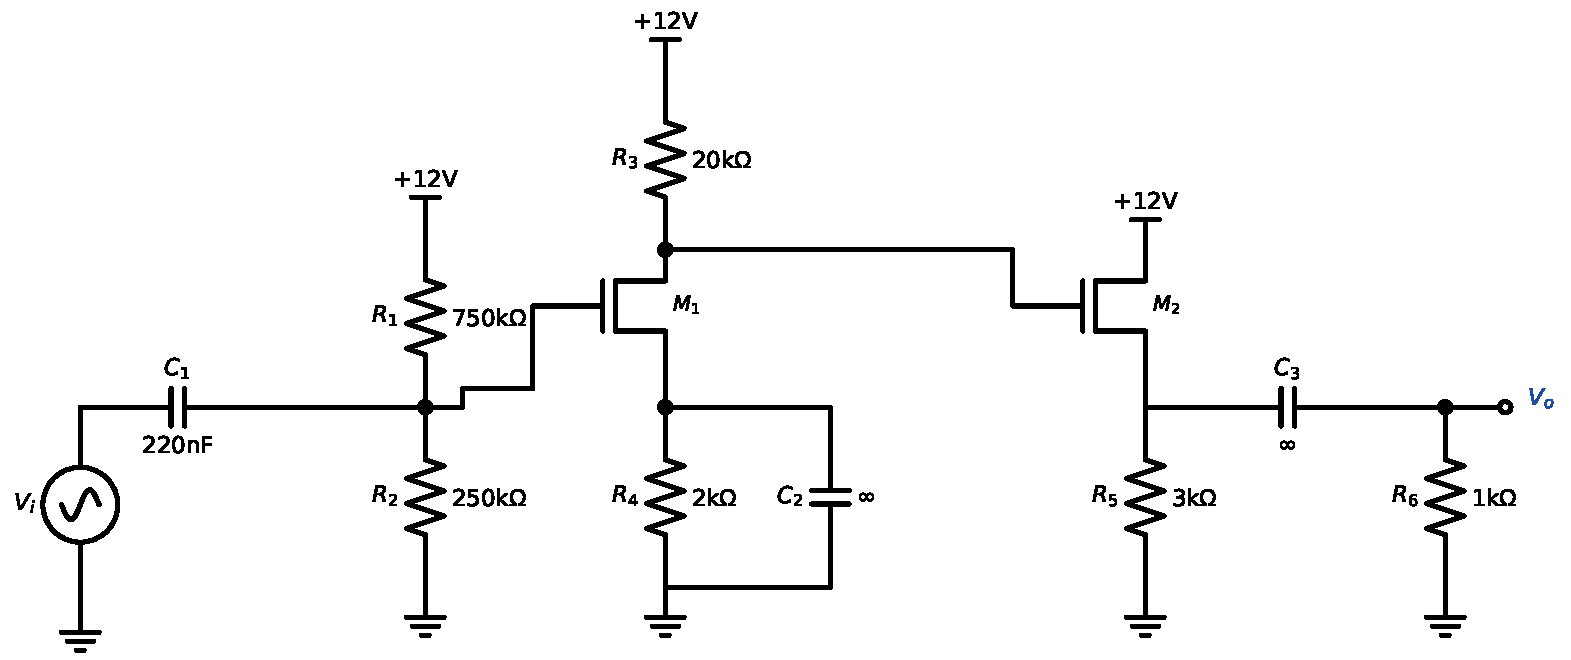
\includegraphics[width=\linewidth,height=7cm,keepaspectratio]{p07_circuit}\end{center}
\end{probbox}

\begin{probbox}{Problem 5D.8 \hfill Medium}
For the amplifier below, find the small-signal transfer function $H(s)=\dfrac{V_o(s)}{V_i(s)}$ and sketch its magnitude Bode plot. Also find the steady-state output $V_o(t)$ for $V_i(t) = 0.005\sin\left(2\pi\cdot 1000\,t\right)$. Assume $k'_n\frac{W}{L} = 1.1\,\mathrm{m}\mathrm{A/V^2}$, $V_{tn} = 1.4$\,V, $k'_p\frac{W}{L} = 850\,\mu \mathrm{A/V^2}$, $V_{tp} = -1.3$\,V, $r_o = \infty$; the DC drain currents are $I_{D1} = 117\,\mu \mathrm{A}$, $I_{D2} = 185\,\mu \mathrm{A}$.
\begin{center}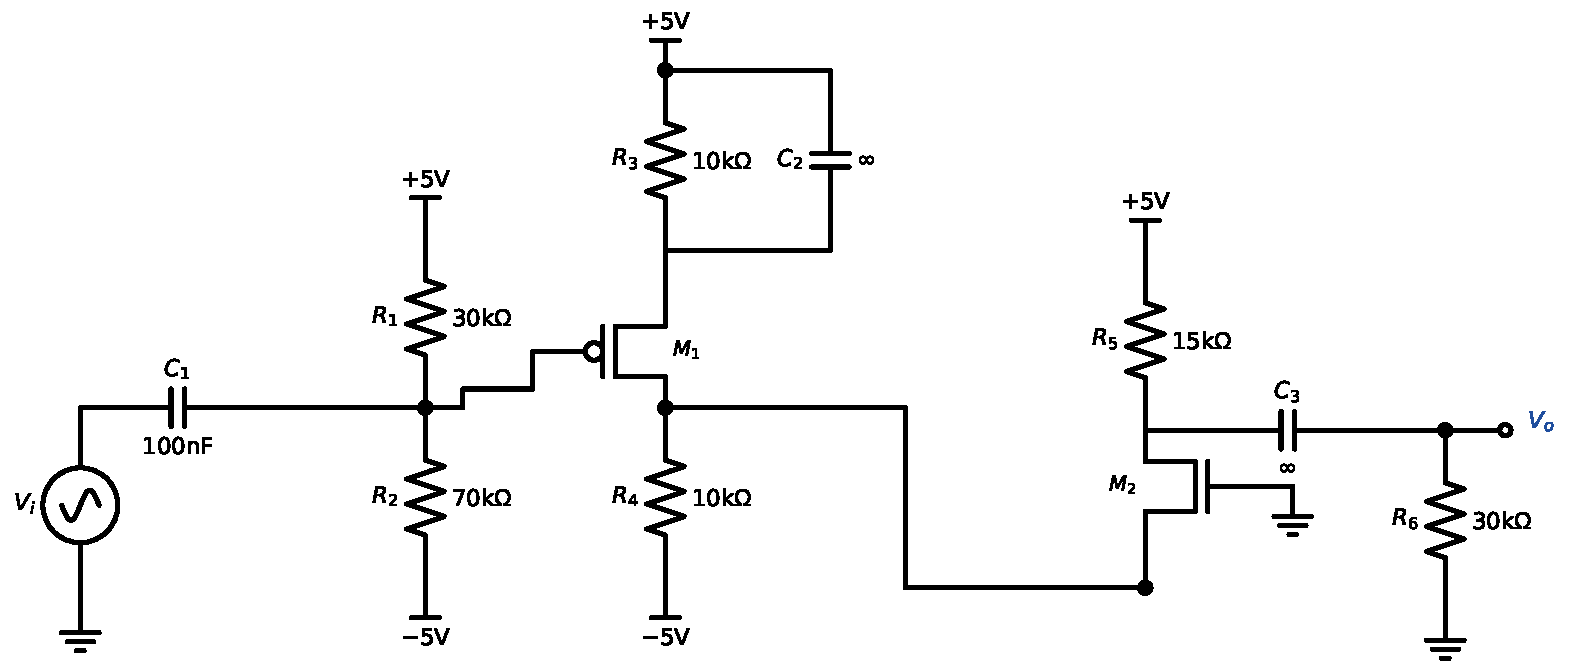
\includegraphics[width=\linewidth,height=7cm,keepaspectratio]{p08_circuit}\end{center}
\end{probbox}

\begin{probbox}{Problem 5D.9 \hfill Medium}
For the amplifier below, find the small-signal transfer function $H(s)=\dfrac{V_o(s)}{V_i(s)}$ and sketch its magnitude Bode plot. Also find the steady-state output $V_o(t)$ for $V_i(t) = 0.01\sin\left(2\pi\cdot 100\,t\right)$. Assume $k'_n\frac{W}{L} = 1.1\,\mathrm{m}\mathrm{A/V^2}$, $V_{tn} = 1.4$\,V, $r_o = \infty$; the DC drain currents are $I_{D1} = 256\,\mu \mathrm{A}$, $I_{D2} = 830\,\mu \mathrm{A}$.
\begin{center}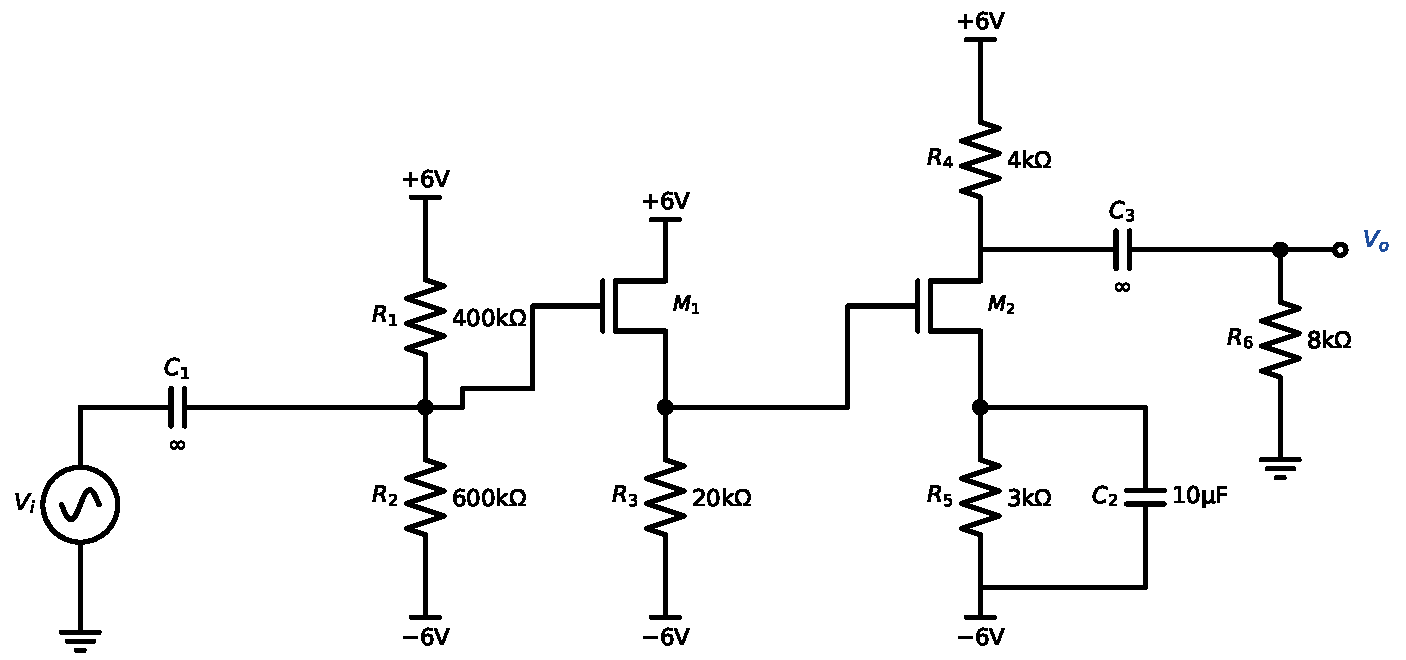
\includegraphics[width=\linewidth,height=7cm,keepaspectratio]{p09_circuit}\end{center}
\end{probbox}

\begin{probbox}{Problem 5D.10 \hfill Medium}
For the amplifier below, find the small-signal transfer function $H(s)=\dfrac{V_o(s)}{V_i(s)}$ and sketch its magnitude Bode plot. Also find the steady-state output $V_o(t)$ for $V_i(t) = 0.002\sin\left(2\pi\cdot 100\,t\right)$. Assume $k'_n\frac{W}{L} = 1.1\,\mathrm{m}\mathrm{A/V^2}$, $V_{tn} = 1.4$\,V, $k'_p\frac{W}{L} = 850\,\mu \mathrm{A/V^2}$, $V_{tp} = -1.3$\,V, $r_o = \infty$; the DC drain currents are $I_{D1} = 200\,\mu \mathrm{A}$, $I_{D2} = 102\,\mu \mathrm{A}$.
\begin{center}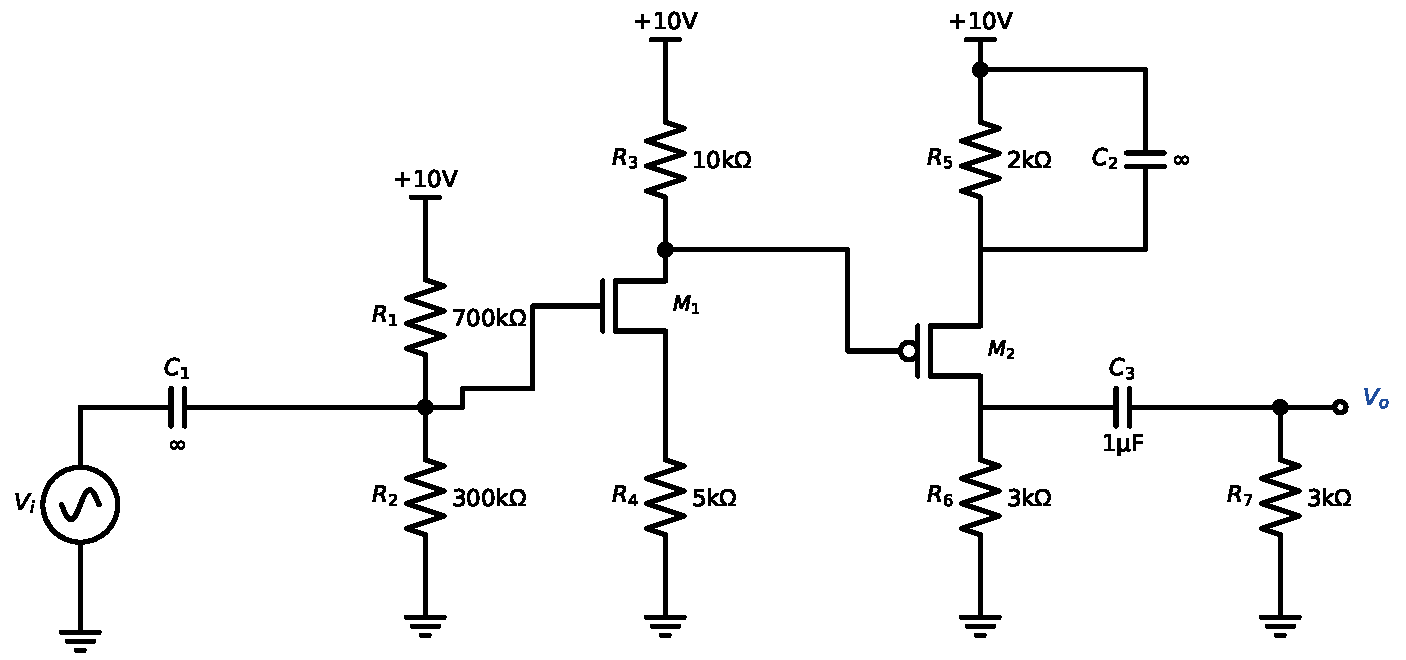
\includegraphics[width=\linewidth,height=7cm,keepaspectratio]{p10_circuit}\end{center}
\end{probbox}

\begin{probbox}{Problem 5D.11 \hfill Medium}
For the amplifier below, find the small-signal transfer function $H(s)=\dfrac{V_o(s)}{V_i(s)}$ and sketch its magnitude Bode plot. Also find the steady-state output $V_o(t)$ for $V_i(t) = 0.005\sin\left(2\pi\cdot 1000\,t\right)$. Assume $k'_n\frac{W}{L} = 2\,\mathrm{m}\mathrm{A/V^2}$, $V_{tn} = 1$\,V, $r_o = \infty$; the DC drain currents are $I_{D1} = 209\,\mu \mathrm{A}$, $I_{D2} = 1.24\,\mathrm{m}\mathrm{A}$.
\begin{center}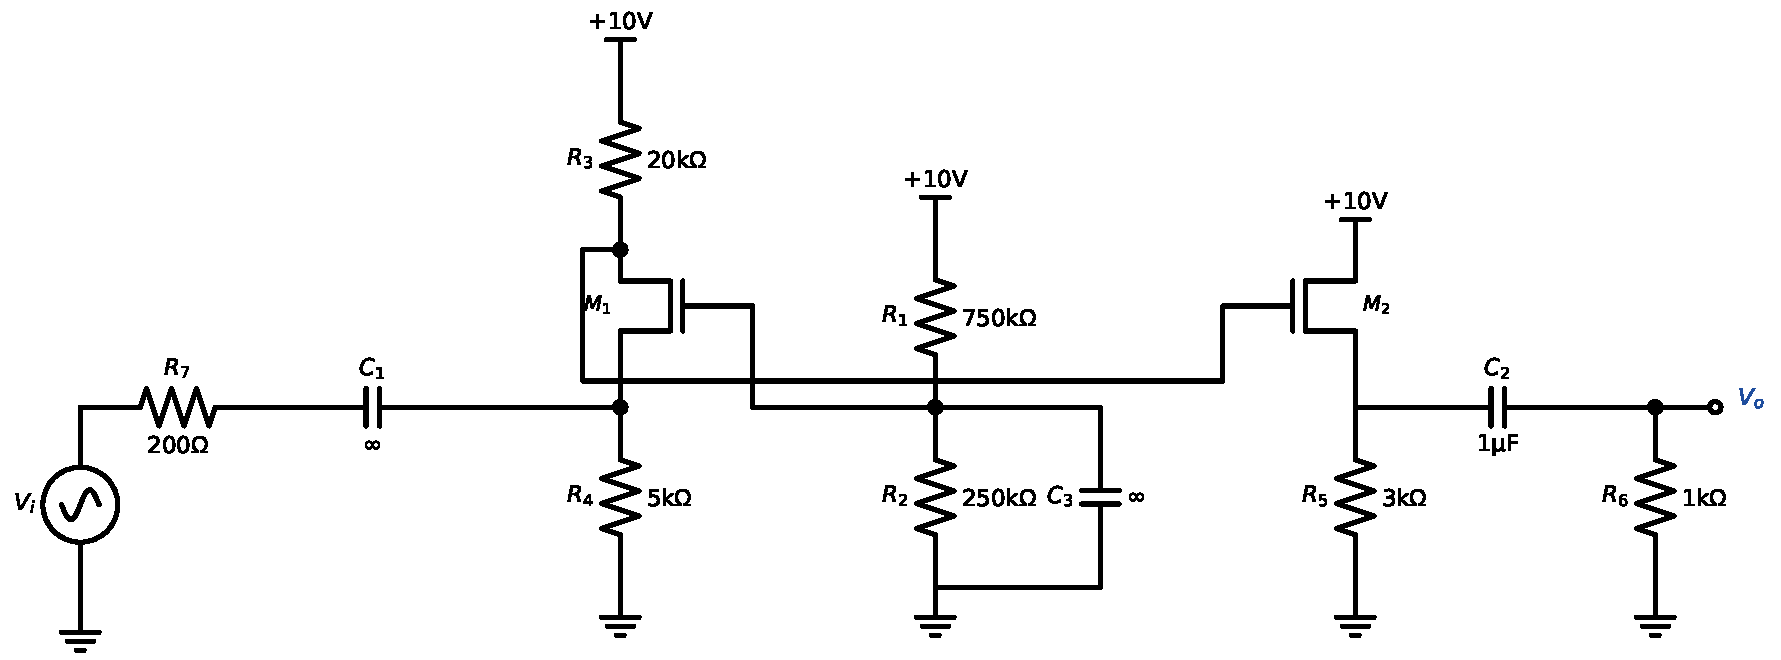
\includegraphics[width=\linewidth,height=7cm,keepaspectratio]{p11_circuit}\end{center}
\end{probbox}

\begin{probbox}{Problem 5D.12 \hfill Medium}
For the amplifier below, find the small-signal transfer function $H(s)=\dfrac{V_o(s)}{V_i(s)}$ and sketch its magnitude Bode plot. Also find the steady-state output $V_o(t)$ for $V_i(t) = 0.005\sin\left(2\pi\cdot 20\,t\right)$. Assume $k'_n\frac{W}{L} = 2\,\mathrm{m}\mathrm{A/V^2}$, $V_{tn} = 1$\,V, $k'_p\frac{W}{L} = 1\,\mathrm{m}\mathrm{A/V^2}$, $V_{tp} = -1$\,V, $r_o = \infty$; the DC drain currents are $I_{D1} = 640\,\mu \mathrm{A}$, $I_{D2} = 357\,\mu \mathrm{A}$.
\begin{center}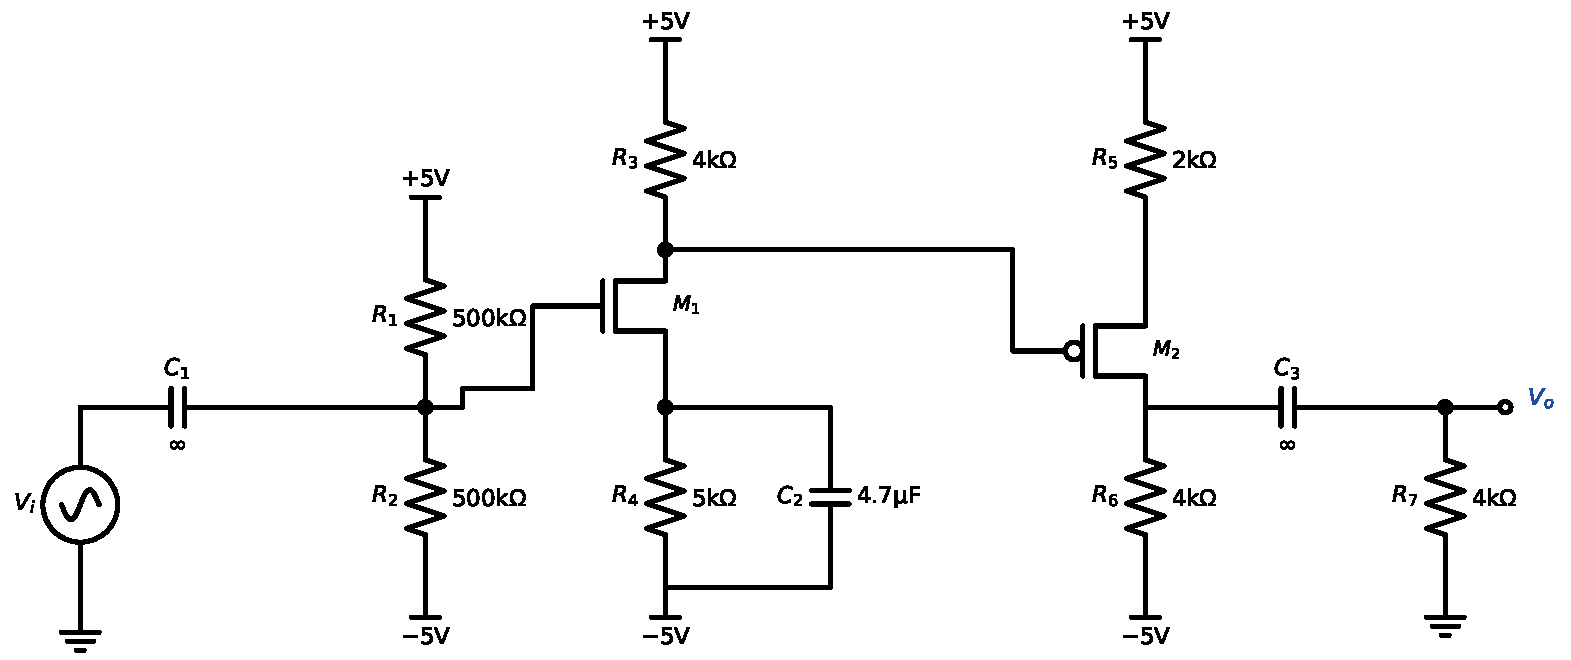
\includegraphics[width=\linewidth,height=7cm,keepaspectratio]{p12_circuit}\end{center}
\end{probbox}

\subsection*{Hard problems}
\begin{probbox}{Problem 5D.13 \hfill Hard}
For the amplifier below, find the small-signal transfer function $H(s)=\dfrac{V_o(s)}{V_i(s)}$ and sketch its magnitude Bode plot. Also find the steady-state output $V_o(t)$ for $V_i(t) = 0.005\sin\left(2\pi\cdot 1000\,t\right)$. Assume $k'_n\frac{W}{L} = 1.1\,\mathrm{m}\mathrm{A/V^2}$, $V_{tn} = 1.4$\,V, $k'_p\frac{W}{L} = 850\,\mu \mathrm{A/V^2}$, $V_{tp} = -1.3$\,V, $r_o = \infty$; the DC drain currents are $I_{D1} = 117\,\mu \mathrm{A}$, $I_{D2} = 185\,\mu \mathrm{A}$, $I_{D3} = 453\,\mu \mathrm{A}$, $I_{D4} = 1.34\,\mathrm{m}\mathrm{A}$. (This is Sample Problem 3 of the lecture.)
\begin{center}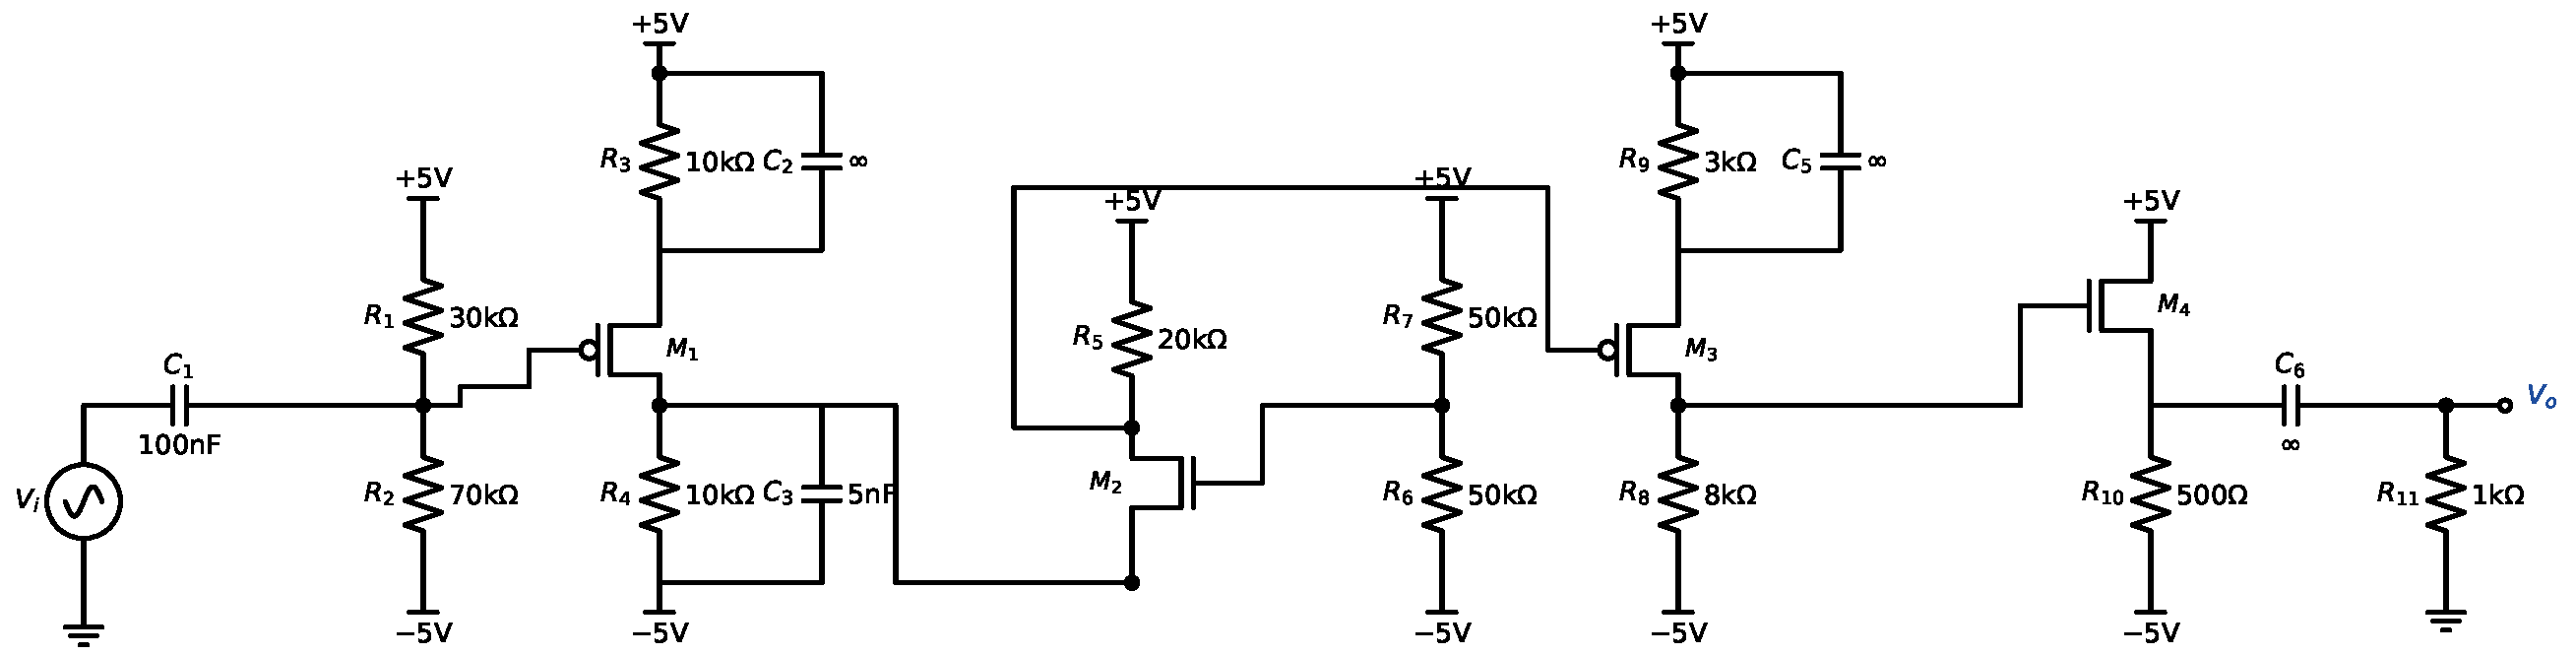
\includegraphics[width=\linewidth,height=7cm,keepaspectratio]{p13_circuit}\end{center}
\end{probbox}

\begin{probbox}{Problem 5D.14 \hfill Hard}
For the amplifier below, find the small-signal transfer function $H(s)=\dfrac{V_o(s)}{V_i(s)}$ and sketch its magnitude Bode plot. Also find the steady-state output $V_o(t)$ for $V_i(t) = 0.01\sin\left(2\pi\cdot 5000\,t\right)$. Assume $k'_n\frac{W}{L} = 1.1\,\mathrm{m}\mathrm{A/V^2}$, $V_{tn} = 1.4$\,V, $k'_p\frac{W}{L} = 850\,\mu \mathrm{A/V^2}$, $V_{tp} = -1.3$\,V, $r_o = \infty$; the DC drain currents are $I_{D2} = 99.4\,\mu \mathrm{A}$, $I_{D3} = 99.4\,\mu \mathrm{A}$, $I_{D4} = 99.4\,\mu \mathrm{A}$, $I_{D6} = 99.4\,\mu \mathrm{A}$. (This is Sample Problem 4 of the lecture.)
\begin{center}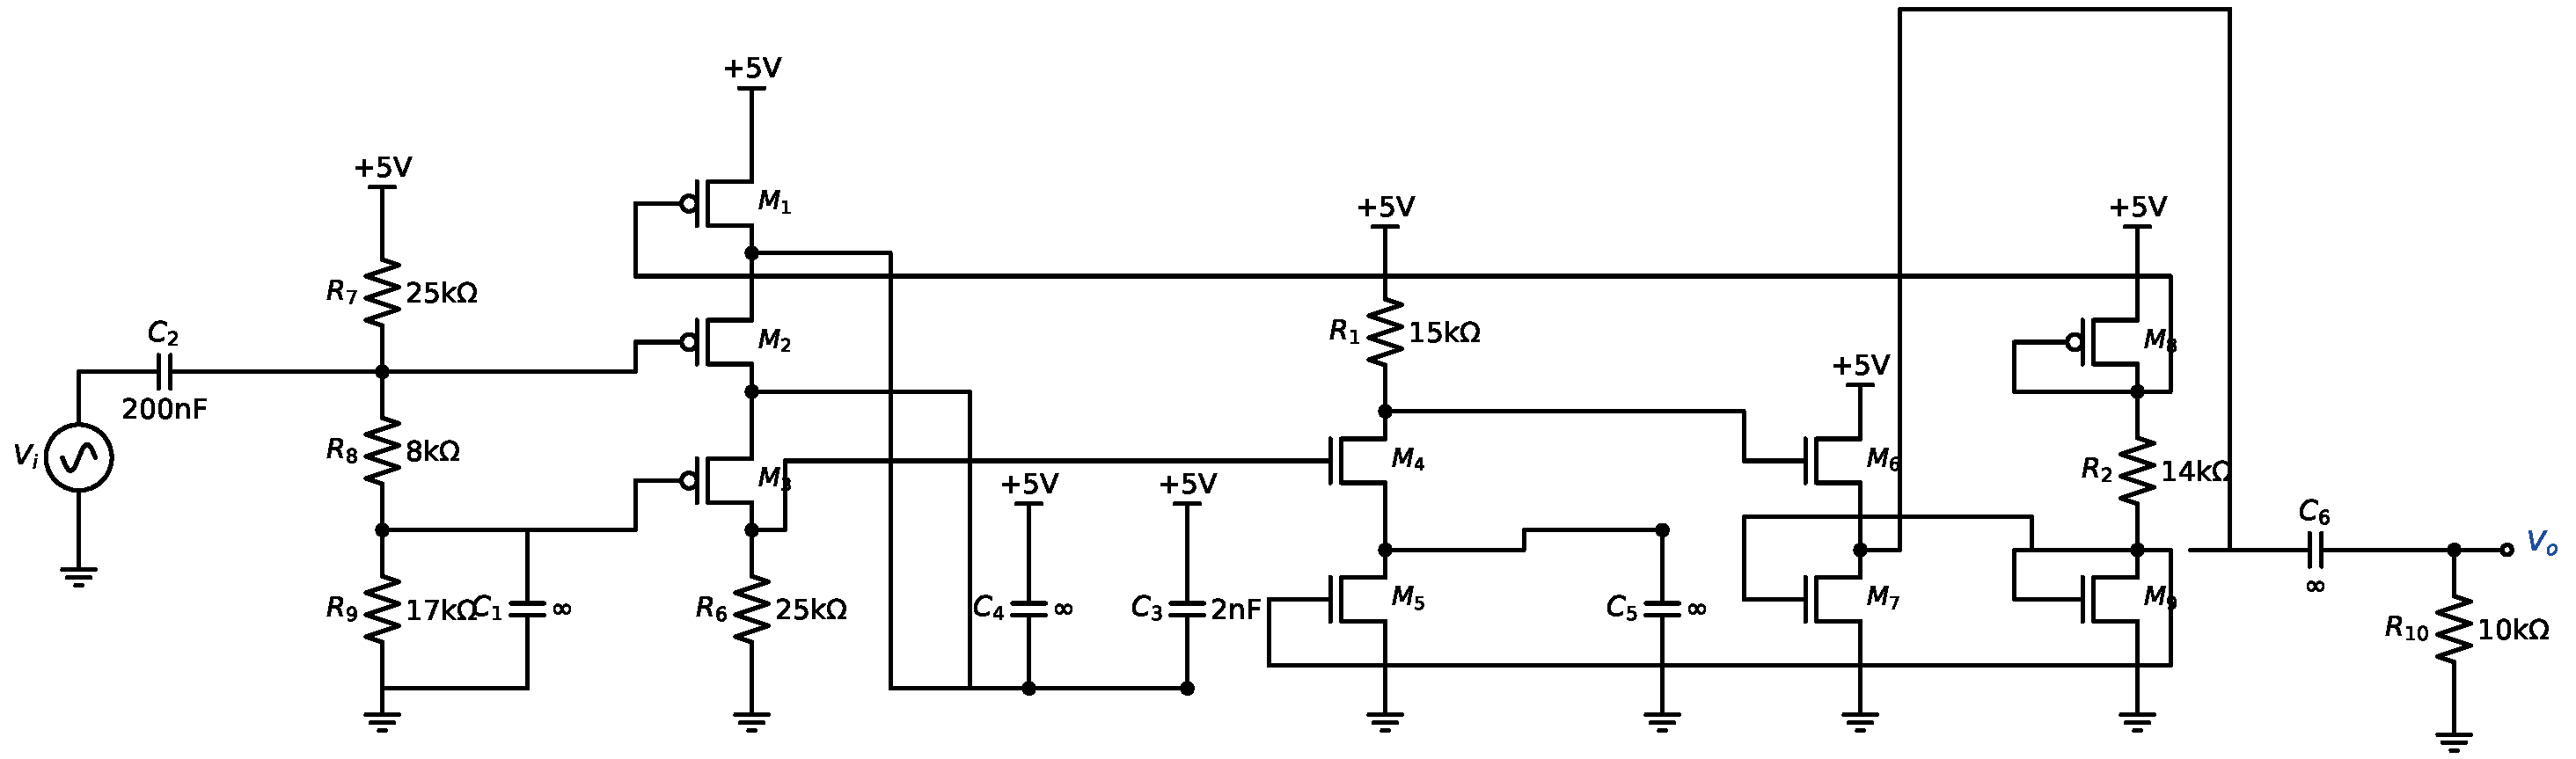
\includegraphics[width=\linewidth,height=7cm,keepaspectratio]{p14_circuit}\end{center}
\end{probbox}

\begin{probbox}{Problem 5D.15 \hfill Hard}
For the amplifier below, find the small-signal transfer function $H(s)=\dfrac{V_o(s)}{V_i(s)}$ and sketch its magnitude Bode plot. Also find the steady-state output $V_o(t)$ for $V_i(t) = 0.001\sin\left(2\pi\cdot 1000\,t\right)$. Assume $k'_n\frac{W}{L} = 1.1\,\mathrm{m}\mathrm{A/V^2}$, $V_{tn} = 1.4$\,V, $k'_p\frac{W}{L} = 850\,\mu \mathrm{A/V^2}$, $V_{tp} = -1.3$\,V, $r_o = \infty$; the DC drain currents are $I_{D1} = 461\,\mu \mathrm{A}$, $I_{D2} = 544\,\mu \mathrm{A}$, $I_{D3} = 1.26\,\mathrm{m}\mathrm{A}$.
\begin{center}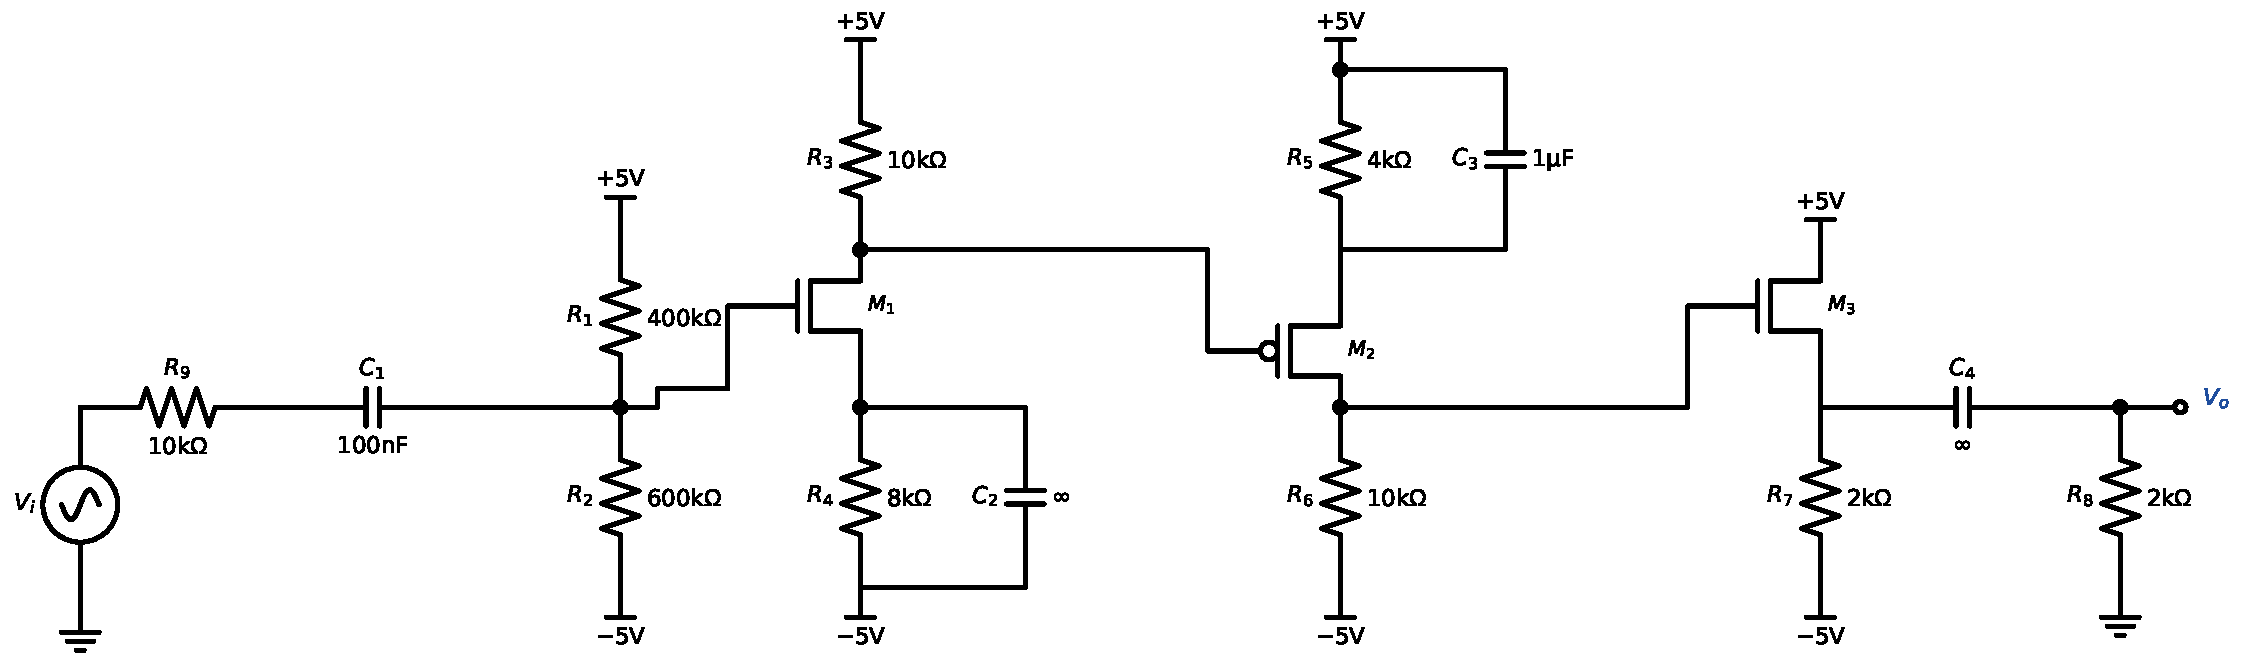
\includegraphics[width=\linewidth,height=7cm,keepaspectratio]{p15_circuit}\end{center}
\end{probbox}

\begin{probbox}{Problem 5D.16 \hfill Hard}
For the amplifier below, find the small-signal transfer function $H(s)=\dfrac{V_o(s)}{V_i(s)}$ and sketch its magnitude Bode plot. Also find the steady-state output $V_o(t)$ for $V_i(t) = 0.001\sin\left(2\pi\cdot 2000\,t\right)$. Assume $k'_n\frac{W}{L} = 1.1\,\mathrm{m}\mathrm{A/V^2}$, $V_{tn} = 1.4$\,V, $k'_p\frac{W}{L} = 850\,\mu \mathrm{A/V^2}$, $V_{tp} = -1.3$\,V, $r_o = \infty$; the DC drain currents are $I_{D1} = 243\,\mu \mathrm{A}$, $I_{D2} = 246\,\mu \mathrm{A}$, $I_{D3} = 518\,\mu \mathrm{A}$, $I_{D4} = 1.24\,\mathrm{m}\mathrm{A}$.
\begin{center}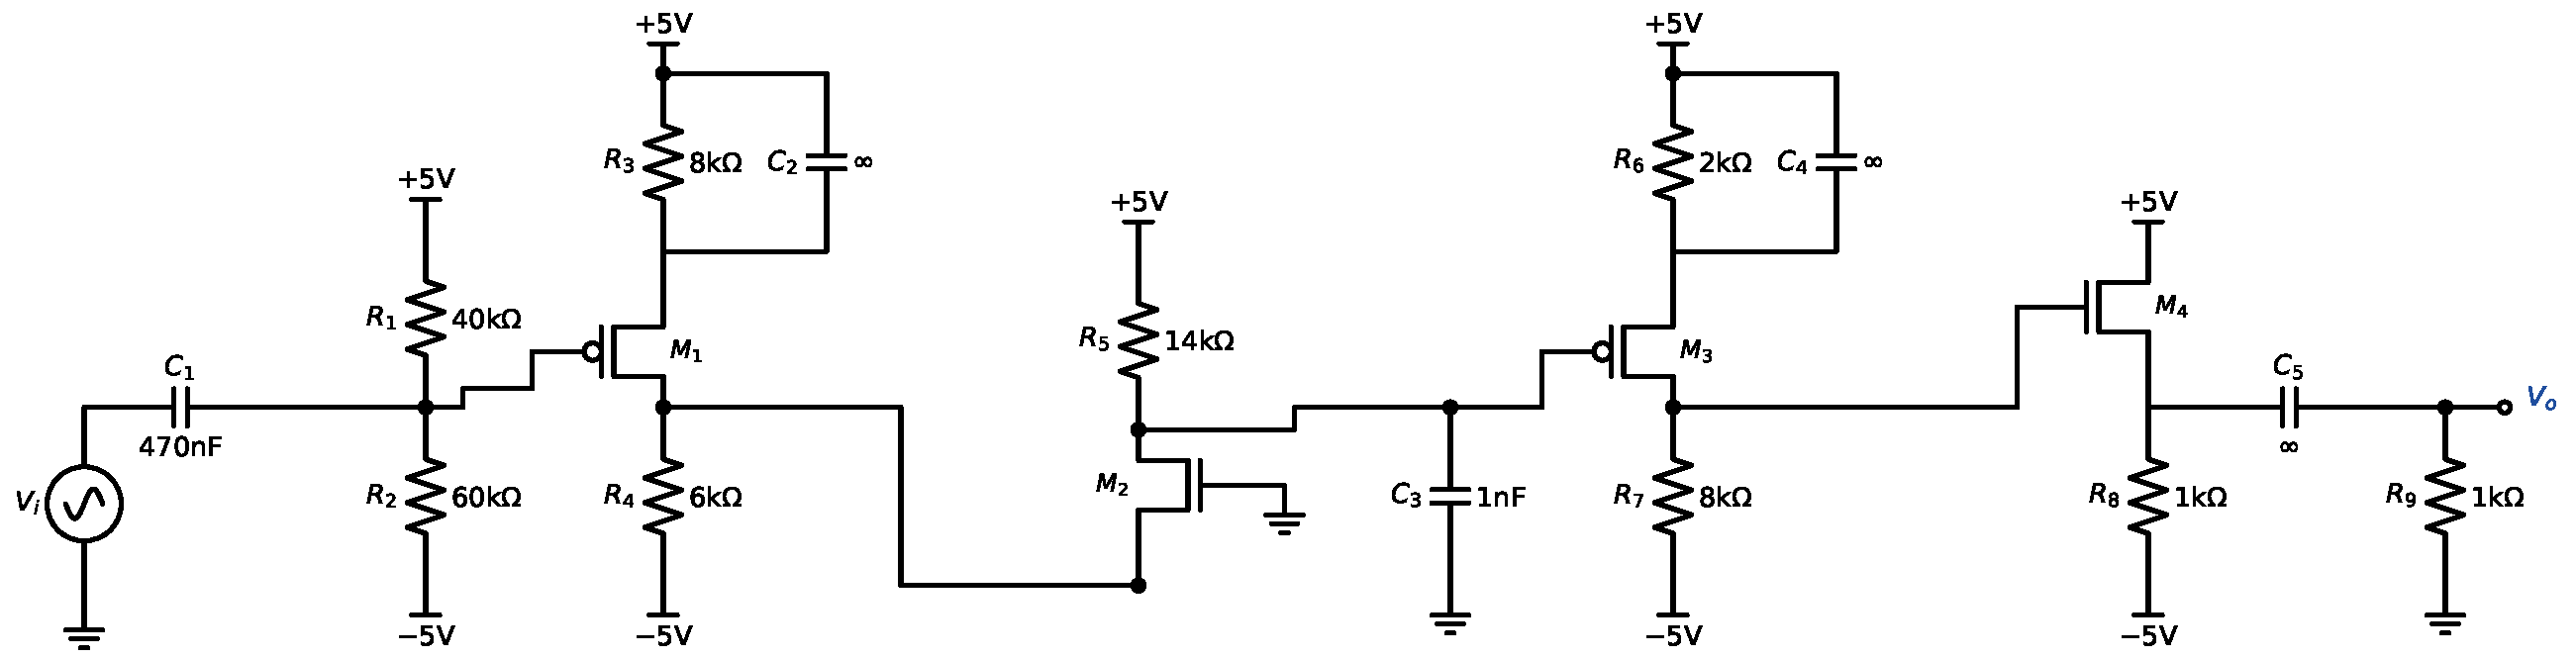
\includegraphics[width=\linewidth,height=7cm,keepaspectratio]{p16_circuit}\end{center}
\end{probbox}

\begin{probbox}{Problem 5D.17 \hfill Hard}
For the amplifier below, find the small-signal transfer function $H(s)=\dfrac{V_o(s)}{V_i(s)}$ and sketch its magnitude Bode plot. Also find the steady-state output $V_o(t)$ for $V_i(t) = 0.01\sin\left(2\pi\cdot 100\,t\right)$. Assume $k'_n = 200\,\mu \mathrm{A/V^2}$, $V_{tn} = 0.7$\,V, $k'_p = 100\,\mu \mathrm{A/V^2}$, $V_{tp} = -0.8$\,V (W/L next to each transistor), $r_o = \infty$; the DC drain currents are $I_{D2} = 373\,\mu \mathrm{A}$, $I_{D4} = 373\,\mu \mathrm{A}$.
\begin{center}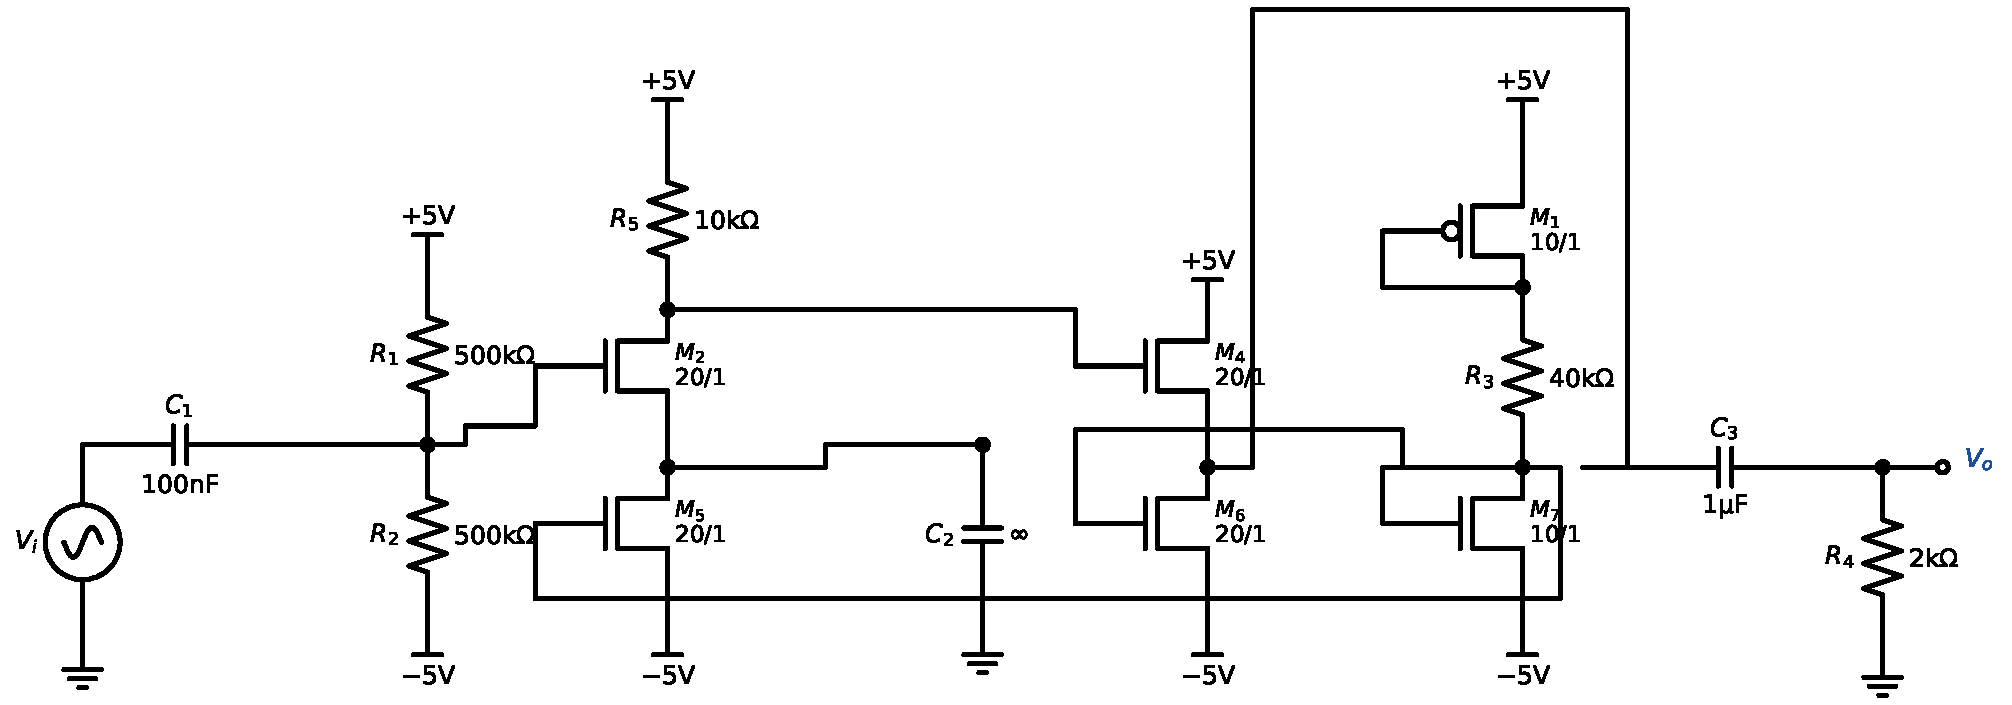
\includegraphics[width=\linewidth,height=7cm,keepaspectratio]{p17_circuit}\end{center}
\end{probbox}

\begin{probbox}{Problem 5D.18 \hfill Hard}
For the amplifier below, find the small-signal transfer function $H(s)=\dfrac{V_o(s)}{V_i(s)}$ and sketch its magnitude Bode plot. Also find the steady-state output $V_o(t)$ for $V_i(t) = 5\times 10^{-4}\sin\left(2\pi\cdot 1000\,t\right)$. Assume $k'_n\frac{W}{L} = 2\,\mathrm{m}\mathrm{A/V^2}$, $V_{tn} = 1$\,V, $k'_p\frac{W}{L} = 1\,\mathrm{m}\mathrm{A/V^2}$, $V_{tp} = -1$\,V, $r_o = \infty$; the DC drain currents are $I_{D1} = 820\,\mu \mathrm{A}$, $I_{D2} = 410\,\mu \mathrm{A}$, $I_{D3} = 445\,\mu \mathrm{A}$, $I_{D4} = 265\,\mu \mathrm{A}$.
\begin{center}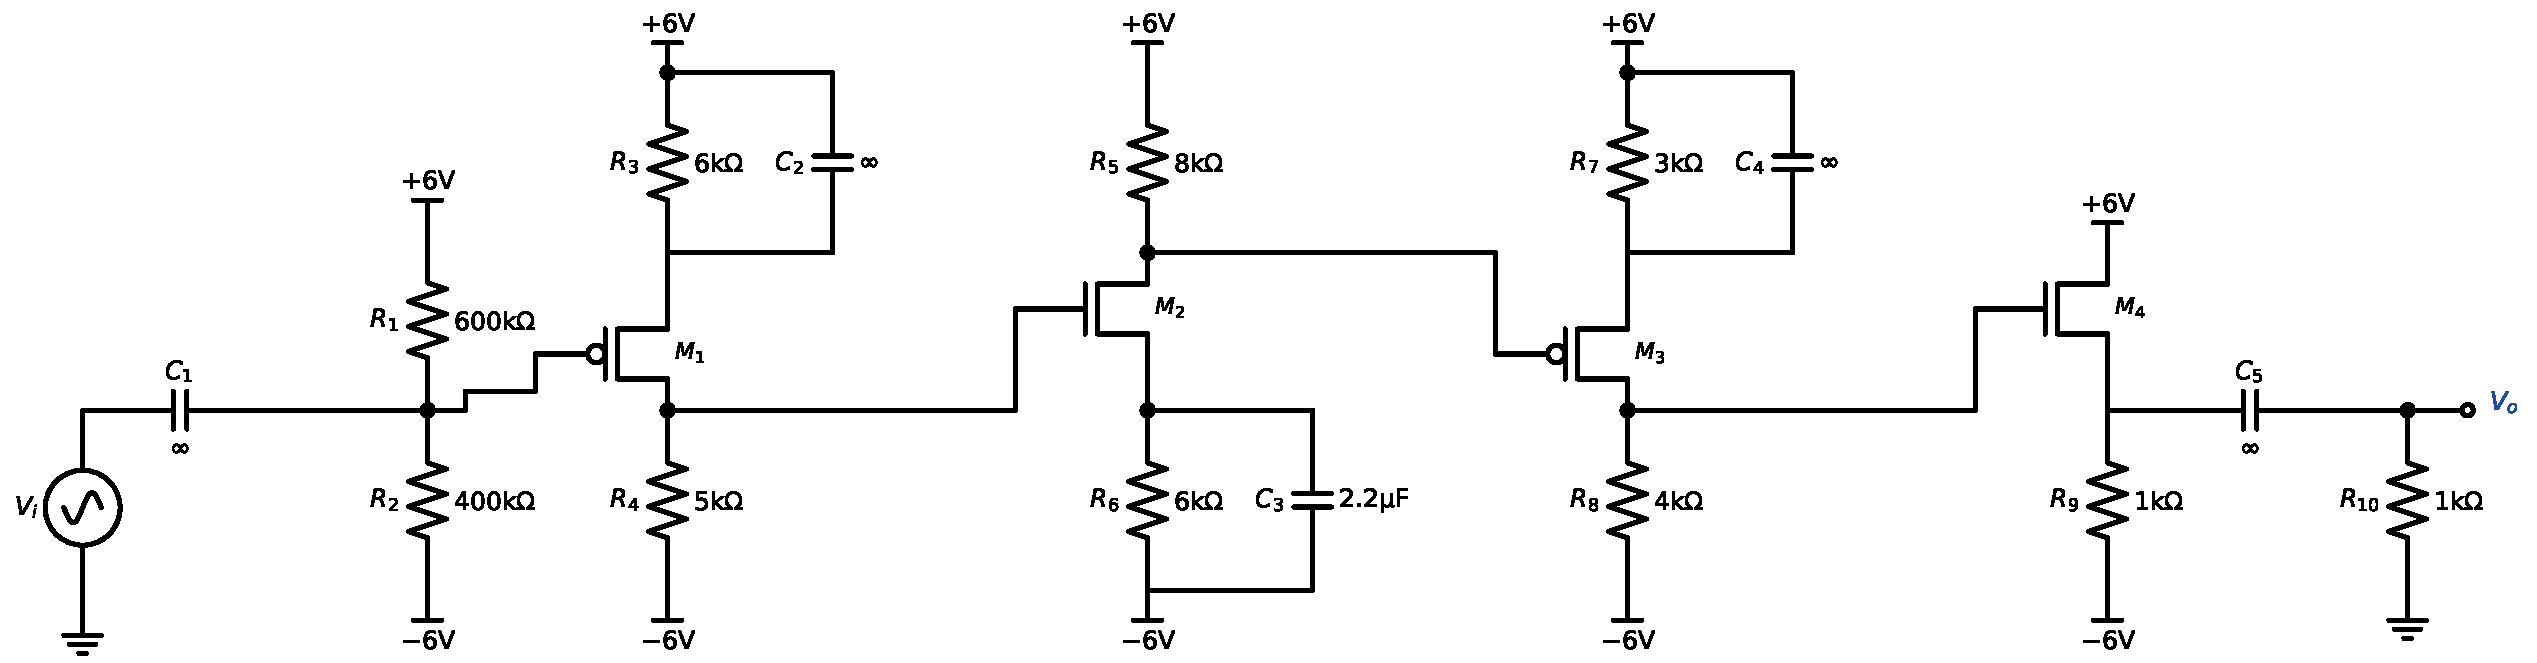
\includegraphics[width=\linewidth,height=7cm,keepaspectratio]{p18_circuit}\end{center}
\end{probbox}

\newpage
\section*{Solutions}
Every solution follows the steps of the Lecture-5 pipeline card.
\subsection*{Solution 5D.1 \hfill Easy}
\begin{center}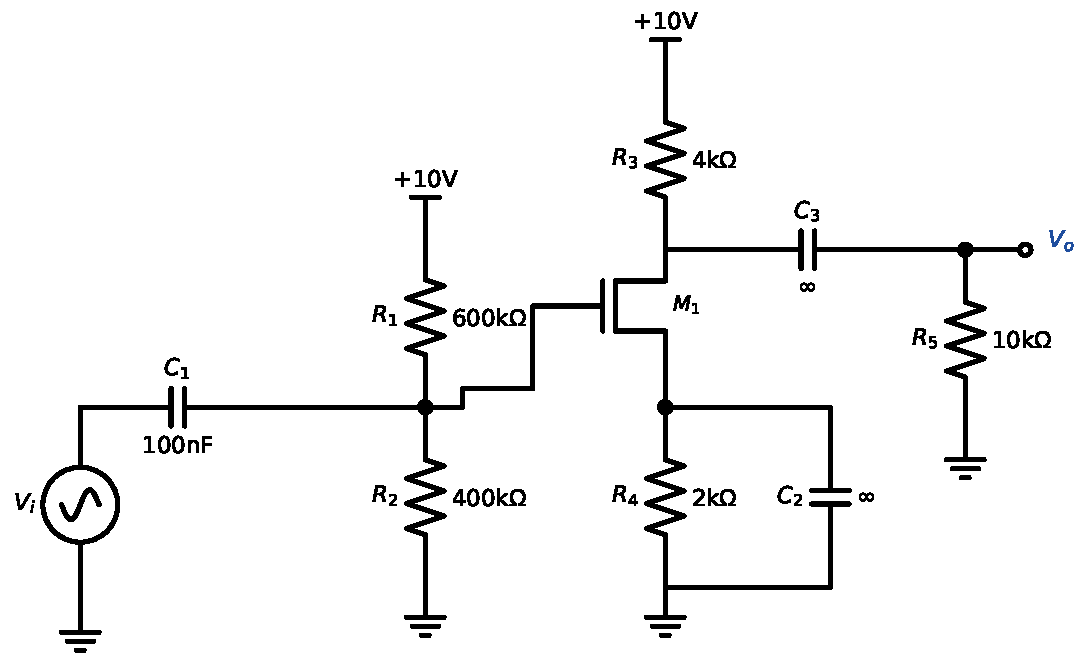
\includegraphics[width=0.9\linewidth,height=6cm,keepaspectratio]{p01_circuit}\end{center}
\solstep{1}{DC currents and transconductances}The DC drain currents are given: $I_{D1} = 726\,\mu \mathrm{A}$. For AC every DC supply is ground and every ``$\infty$'' capacitor is a short. Transconductances (tool T4):\begin{align*}
g_{m1} &= k_{1}V_{ov1} = \sqrt{2k_{1}I_{D1}} = \sqrt{2\cdot1.1\,\mathrm{m}\mathrm{A/V^2}\cdot726\,\mu \mathrm{A}} = 1.26\,\mathrm{m}\mathrm{A/V},\qquad \frac{1}{g_{m1}} = 791\,\Omega\quad(V_{ov1} = 1.15\,\mathrm{V})
\end{align*}

\solstep{2}{Input resistance of each stage}Input resistance of every stage, from the last back to the first (each one loads the stage before it):\begin{align*}
R_{i1} &= Z_{gate,1} = \infty\quad\text{(input at the gate: it loads nothing)}
\end{align*}

\solstep{3}{Gain along the signal path}Multiply the node-to-node gains along the signal path (tool T4):\[
H(s) = \frac{v_{g1}}{v_i}\cdot\frac{v_{d1}}{v_{g1}}
\]
\begin{align*}
\frac{v_{g1}}{v_i} &= \frac{R_{1} \parallel R_{2}}{\frac{1}{sC_{1}} + R_{1} \parallel R_{2}} = \dfrac{s}{s + 41.7} \\
\frac{v_{d1}}{v_{g1}} &= -\frac{Z_{D1}}{1/g_{m1} + Z_{S1}},\quad Z_{D1} = R_{3} \parallel R_{5},\ Z_{S1} = 0\ \Rightarrow\ -3.61
\end{align*}

\solstep{4}{Transfer function}Multiply and simplify:\[
H(s) = \dfrac{-3.61\,s}{s + 41.7}
\]

\solstep{5}{Standard (Bode-ready) form}Find the roots. Every root $s=-p$ of the denominator is a \emph{pole}, every root $s=-z$ of the numerator is a \emph{zero}; $|p|$ and $|z|$ are the corner frequencies (rad/s).
\begin{itemize}[leftmargin=*,itemsep=2pt]
\item Numerator: it has the factor $s$ $\Rightarrow$ 1 zero at $s=0$.
\item Denominator: $s + 41.7$; $s + 41.7 = 0 \Rightarrow s = -41.7$.
\end{itemize}

Factored form (leading coefficient in front):
\[
H(s) = -3.61\,\dfrac{s}{(s+41.7)}
\]

Bode-ready form: rewrite every $(s+p) = p\left(1+\frac{s}{p}\right)$ and $(s+z) = z\left(1+\frac{s}{z}\right)$, and collect all constants into $K$. Each $s$ in the numerator is paired with one of the \emph{lowest} poles as $\frac{s}{s+p}$ (that factor is $\approx 1$ above $p$). Then every factor except $K$ is $\approx 1$ inside the pass-band:
\[
H(s) = -3.61\,\dfrac{s}{s+2\pi\cdot 6.63},\qquad K = -3.61
\]

\begin{center}\renewcommand{\arraystretch}{1.35}
\begin{tabular}{cccc}
\toprule
type & $\omega_c$ (rad/s) & $f_c=\omega_c/2\pi$ & slope change \\
\midrule
pole & $41.7$ & 6.63 Hz & $-20$ dB/dec \\
\bottomrule
\end{tabular}\end{center}

\solstep{6}{Magnitude Bode plot}Below every corner $|H(s)|\approx 0.0866\,s$, so the plot starts with a slope of $+20$\,dB/dec. Then, moving right, each pole bends the line down by 20\,dB/dec and each zero bends it up by 20\,dB/dec (tool T6):
\begin{center}\renewcommand{\arraystretch}{1.35}
\begin{tabular}{lcl}
\toprule
frequency range & slope & asymptote level \\
\midrule
$f<$ 6.63 Hz & $+20$ dB/dec & 11.2 dB at end \\
$f>$ 6.63 Hz & $0$ dB/dec (flat) & 11.2 dB at start \\
\bottomrule
\end{tabular}\end{center}

The flat (pass-band) level is $20\log_{10}|K| = 20\log_{10}3.61 = 11.2$\,dB.
\begin{center}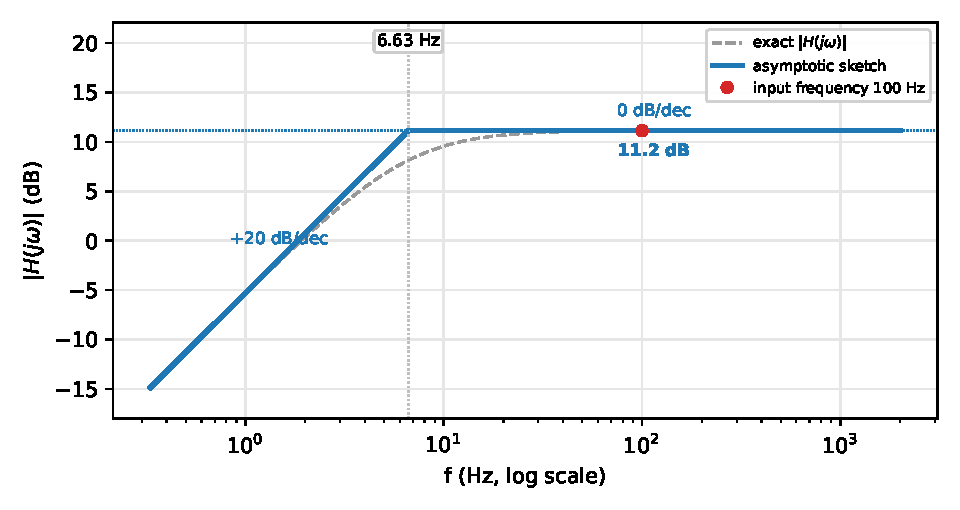
\includegraphics[width=0.78\linewidth,height=6.5cm,keepaspectratio]{p01_bode}\end{center}

{\small Blue: the straight-line sketch you are expected to draw. Dashed grey: the exact curve (about 3\,dB below the corner of an isolated pole). Red dot: the input frequency of Step 7.}
\solstep{7}{Steady-state output}The input is $V_i(t) = 0.01\sin\left(2\pi\cdot 100\,t\right)$, so $\omega_{in} = 2\pi\cdot 100 = 628$\,rad/s. Put $s=j\omega_{in}$ in each factor (tool T5): magnitudes multiply, angles add.
{\small Rules: $\left|\frac{s}{s+p}\right| = \frac{\omega}{\sqrt{\omega^2+p^2}}$, $\angle = \frac{\pi}{2}-\tan^{-1}\frac{\omega}{p}$;\quad $\left|\frac{1}{1+s/p}\right| = \frac{1}{\sqrt{1+(\omega/p)^2}}$, $\angle = -\tan^{-1}\frac{\omega}{p}$;\quad $\left|1+\frac{s}{z}\right| = \sqrt{1+(\omega/z)^2}$, $\angle = \tan^{-1}\frac{\omega}{z}$;\quad a negative $K$ adds $-\pi$.}
\begin{center}\renewcommand{\arraystretch}{1.35}
\begin{tabular}{ccc}
\toprule
factor & magnitude & angle (rad) \\
\midrule
$-3.61$ & $3.61$ & $-3.14$ \\
$\rule[-1.1em]{0pt}{2.8em}\dfrac{s}{s+2\pi\cdot 6.63}$ & $0.9978$ & $0.0662$ \\
\textbf{total} & $\mathbf{3.602}$ (product) & $\mathbf{-3.08}$ (sum) \\
\bottomrule
\end{tabular}\end{center}

\begin{align*}
|H(j\omega_{in})| &= 3.6, \qquad \angle H(j\omega_{in}) = -3.08\ \mathrm{rad} \\
v_{o,ac}(t) &= 3.6\times 0.01\,\sin\left(2\pi\cdot 100\,t - 3.08\right) = 0.036\,\sin\left(2\pi\cdot 100\,t - 3.08\right)
\end{align*}

\[
\boxed{V_o(t) = 0.036\,\sin\left(2\pi\cdot 100\,t - 3.08\right)\ \mathrm{V}}
\]

\begin{ansbox}
$H(s) = -3.61\,\dfrac{s}{s+2\pi\cdot 6.63}$\quad (corners: 6.63 Hz)\\[4pt]
$V_o(t) = 0.036\,\sin\left(2\pi\cdot 100\,t - 3.08\right)\ \mathrm{V}$
\end{ansbox}

\newpage
\subsection*{Solution 5D.2 \hfill Easy}
\begin{center}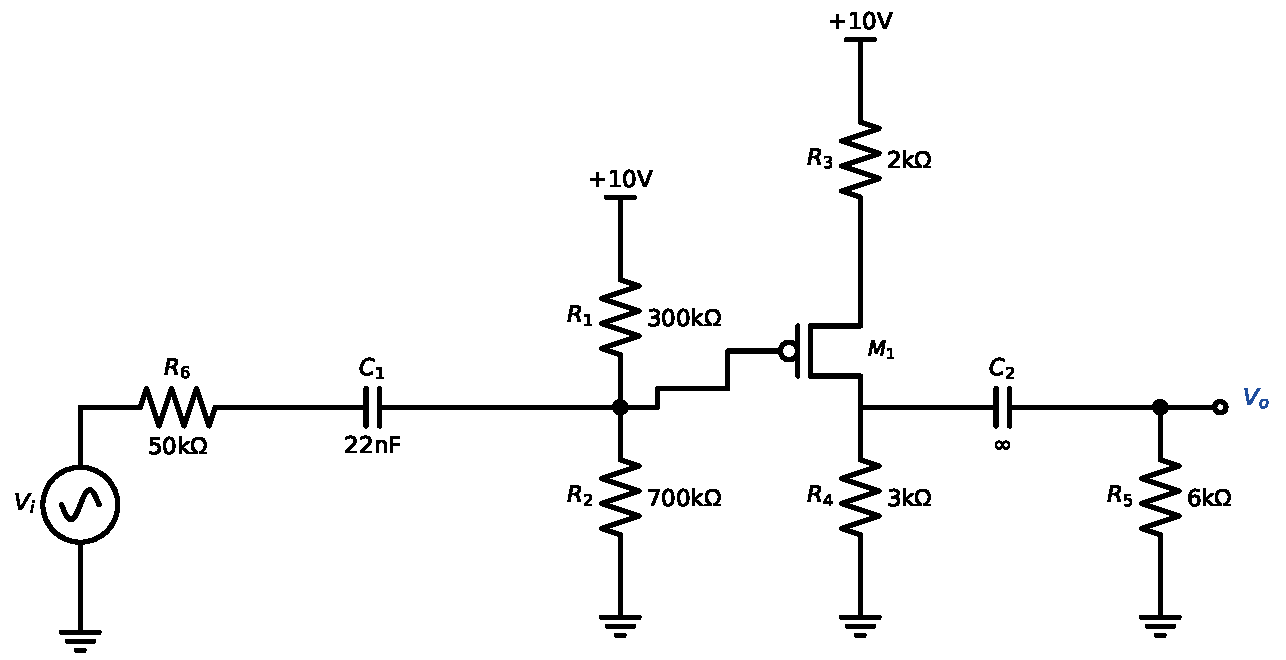
\includegraphics[width=0.9\linewidth,height=6cm,keepaspectratio]{p02_circuit}\end{center}
\solstep{1}{DC currents and transconductances}The DC drain currents are given: $I_{D1} = 378\,\mu \mathrm{A}$. For AC every DC supply is ground and every ``$\infty$'' capacitor is a short. Transconductances (tool T4):\begin{align*}
g_{m1} &= k_{1}V_{ov1} = \sqrt{2k_{1}I_{D1}} = \sqrt{2\cdot850\,\mu \mathrm{A/V^2}\cdot378\,\mu \mathrm{A}} = 802\,\mu \mathrm{A/V},\qquad \frac{1}{g_{m1}} = 1.25\,\mathrm{k}\Omega\quad(V_{ov1} = 0.943\,\mathrm{V})
\end{align*}

\solstep{2}{Input resistance of each stage}Input resistance of every stage, from the last back to the first (each one loads the stage before it):\begin{align*}
R_{i1} &= Z_{gate,1} = \infty\quad\text{(input at the gate: it loads nothing)}
\end{align*}

\solstep{3}{Gain along the signal path}Multiply the node-to-node gains along the signal path (tool T4):\[
H(s) = \frac{v_{g1}}{v_i}\cdot\frac{v_{d1}}{v_{g1}}
\]
\begin{align*}
\frac{v_{g1}}{v_i} &= \frac{R_{1} \parallel R_{2}}{R_{6} + \frac{1}{sC_{1}} + R_{1} \parallel R_{2}} = \dfrac{0.808\,s}{s + 175} \\
\frac{v_{d1}}{v_{g1}} &= -\frac{Z_{D1}}{1/g_{m1} + Z_{S1}},\quad Z_{D1} = R_{4} \parallel R_{5},\ Z_{S1} = R_{3}\ \Rightarrow\ -0.616
\end{align*}

\solstep{4}{Transfer function}Multiply and simplify:\[
H(s) = \dfrac{-0.497\,s}{s + 175}
\]

\solstep{5}{Standard (Bode-ready) form}Find the roots. Every root $s=-p$ of the denominator is a \emph{pole}, every root $s=-z$ of the numerator is a \emph{zero}; $|p|$ and $|z|$ are the corner frequencies (rad/s).
\begin{itemize}[leftmargin=*,itemsep=2pt]
\item Numerator: it has the factor $s$ $\Rightarrow$ 1 zero at $s=0$.
\item Denominator: $s + 175$; $s + 175 = 0 \Rightarrow s = -175$.
\end{itemize}

Factored form (leading coefficient in front):
\[
H(s) = -0.497\,\dfrac{s}{(s+175)}
\]

Bode-ready form: rewrite every $(s+p) = p\left(1+\frac{s}{p}\right)$ and $(s+z) = z\left(1+\frac{s}{z}\right)$, and collect all constants into $K$. Each $s$ in the numerator is paired with one of the \emph{lowest} poles as $\frac{s}{s+p}$ (that factor is $\approx 1$ above $p$). Then every factor except $K$ is $\approx 1$ inside the pass-band:
\[
H(s) = -0.497\,\dfrac{s}{s+2\pi\cdot 27.8},\qquad K = -0.497
\]

\begin{center}\renewcommand{\arraystretch}{1.35}
\begin{tabular}{cccc}
\toprule
type & $\omega_c$ (rad/s) & $f_c=\omega_c/2\pi$ & slope change \\
\midrule
pole & $175$ & 27.8 Hz & $-20$ dB/dec \\
\bottomrule
\end{tabular}\end{center}

\solstep{6}{Magnitude Bode plot}Below every corner $|H(s)|\approx 0.00285\,s$, so the plot starts with a slope of $+20$\,dB/dec. Then, moving right, each pole bends the line down by 20\,dB/dec and each zero bends it up by 20\,dB/dec (tool T6):
\begin{center}\renewcommand{\arraystretch}{1.35}
\begin{tabular}{lcl}
\toprule
frequency range & slope & asymptote level \\
\midrule
$f<$ 27.8 Hz & $+20$ dB/dec & -6.06 dB at end \\
$f>$ 27.8 Hz & $0$ dB/dec (flat) & -6.06 dB at start \\
\bottomrule
\end{tabular}\end{center}

The flat (pass-band) level is $20\log_{10}|K| = 20\log_{10}0.497 = -6.06$\,dB.
\begin{center}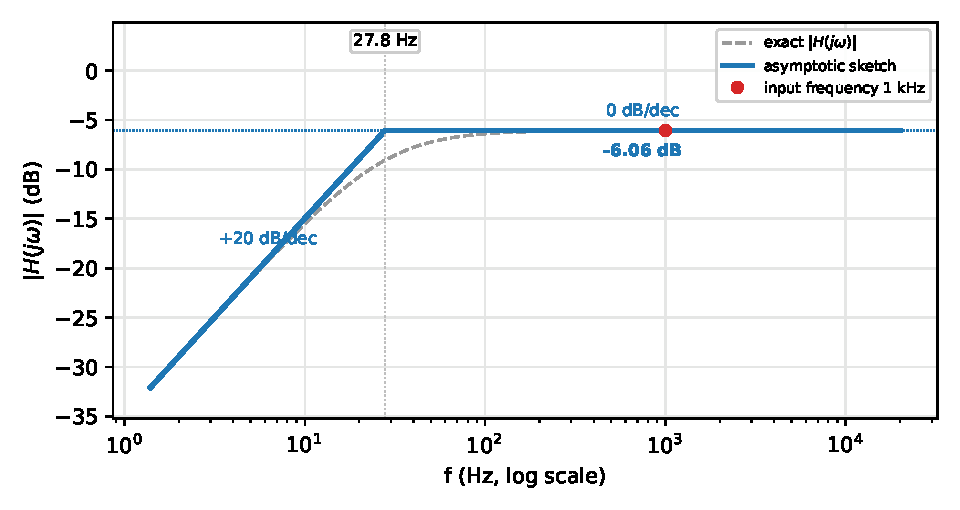
\includegraphics[width=0.78\linewidth,height=6.5cm,keepaspectratio]{p02_bode}\end{center}

{\small Blue: the straight-line sketch you are expected to draw. Dashed grey: the exact curve (about 3\,dB below the corner of an isolated pole). Red dot: the input frequency of Step 7.}
\solstep{7}{Steady-state output}The input is $V_i(t) = 0.02\sin\left(2\pi\cdot 1000\,t\right)$, so $\omega_{in} = 2\pi\cdot 1000 = 6280$\,rad/s. Put $s=j\omega_{in}$ in each factor (tool T5): magnitudes multiply, angles add.
{\small Rules: $\left|\frac{s}{s+p}\right| = \frac{\omega}{\sqrt{\omega^2+p^2}}$, $\angle = \frac{\pi}{2}-\tan^{-1}\frac{\omega}{p}$;\quad $\left|\frac{1}{1+s/p}\right| = \frac{1}{\sqrt{1+(\omega/p)^2}}$, $\angle = -\tan^{-1}\frac{\omega}{p}$;\quad $\left|1+\frac{s}{z}\right| = \sqrt{1+(\omega/z)^2}$, $\angle = \tan^{-1}\frac{\omega}{z}$;\quad a negative $K$ adds $-\pi$.}
\begin{center}\renewcommand{\arraystretch}{1.35}
\begin{tabular}{ccc}
\toprule
factor & magnitude & angle (rad) \\
\midrule
$-0.497$ & $0.4975$ & $-3.14$ \\
$\rule[-1.1em]{0pt}{2.8em}\dfrac{s}{s+2\pi\cdot 27.8}$ & $0.9996$ & $0.0278$ \\
\textbf{total} & $\mathbf{0.4973}$ (product) & $\mathbf{-3.11}$ (sum) \\
\bottomrule
\end{tabular}\end{center}

\begin{align*}
|H(j\omega_{in})| &= 0.497, \qquad \angle H(j\omega_{in}) = -3.11\ \mathrm{rad} \\
v_{o,ac}(t) &= 0.497\times 0.02\,\sin\left(2\pi\cdot 1000\,t - 3.11\right) = 0.00995\,\sin\left(2\pi\cdot 1000\,t - 3.11\right)
\end{align*}

\[
\boxed{V_o(t) = 0.00995\,\sin\left(2\pi\cdot 1000\,t - 3.11\right)\ \mathrm{V}}
\]

\begin{ansbox}
$H(s) = -0.497\,\dfrac{s}{s+2\pi\cdot 27.8}$\quad (corners: 27.8 Hz)\\[4pt]
$V_o(t) = 0.00995\,\sin\left(2\pi\cdot 1000\,t - 3.11\right)\ \mathrm{V}$
\end{ansbox}

\newpage
\subsection*{Solution 5D.3 \hfill Easy}
\begin{center}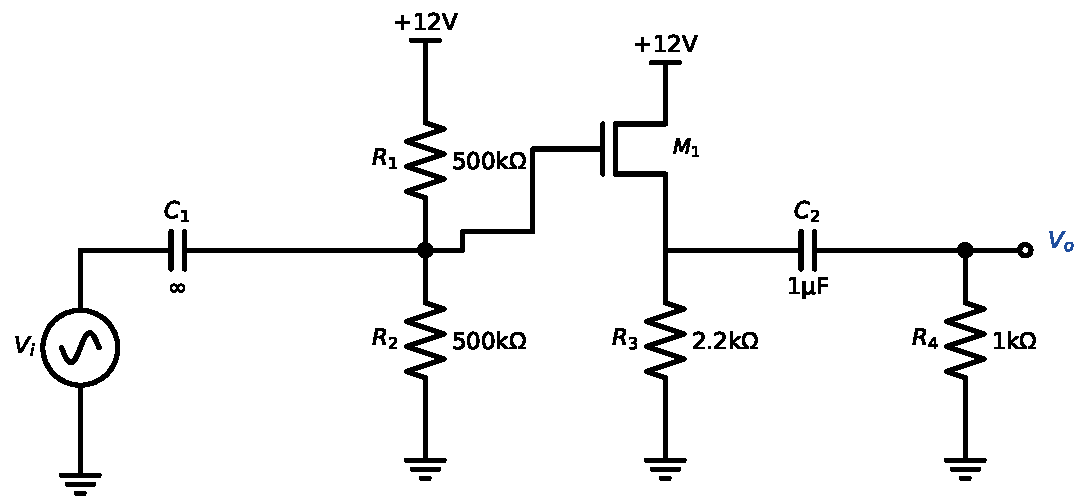
\includegraphics[width=0.9\linewidth,height=6cm,keepaspectratio]{p03_circuit}\end{center}
\solstep{1}{DC currents and transconductances}The DC drain currents are given: $I_{D1} = 1.37\,\mathrm{m}\mathrm{A}$. For AC every DC supply is ground and every ``$\infty$'' capacitor is a short. Transconductances (tool T4):\begin{align*}
g_{m1} &= k_{1}V_{ov1} = \sqrt{2k_{1}I_{D1}} = \sqrt{2\cdot1.1\,\mathrm{m}\mathrm{A/V^2}\cdot1.37\,\mathrm{m}\mathrm{A}} = 1.74\,\mathrm{m}\mathrm{A/V},\qquad \frac{1}{g_{m1}} = 575\,\Omega\quad(V_{ov1} = 1.58\,\mathrm{V})
\end{align*}

\solstep{2}{Input resistance of each stage}Input resistance of every stage, from the last back to the first (each one loads the stage before it):\begin{align*}
R_{i1} &= Z_{gate,1} = \infty\quad\text{(input at the gate: it loads nothing)}
\end{align*}

\solstep{3}{Gain along the signal path}Multiply the node-to-node gains along the signal path (tool T4):\[
H(s) = \frac{v_{s1}}{v_{g1}}\cdot\frac{v_o}{v_{s1}}
\]
\begin{align*}
\frac{v_{s1}}{v_{g1}} &= \frac{Z_{S1}}{1/g_{m1} + Z_{S1}},\quad Z_{S1} = R_{3} \parallel \left(\frac{1}{sC_{2}} + R_{4}\right)\ \Rightarrow\ \dfrac{0.544\,s + 544}{s + 687} \\
\frac{v_o}{v_{s1}} &= \frac{R_{4}}{\frac{1}{sC_{2}} + R_{4}} = \dfrac{s}{s + 1000}
\end{align*}

\solstep{4}{Transfer function}Multiply and simplify:\[
H(s) = \dfrac{0.544\,s}{s + 687}
\]

\solstep{5}{Standard (Bode-ready) form}Find the roots. Every root $s=-p$ of the denominator is a \emph{pole}, every root $s=-z$ of the numerator is a \emph{zero}; $|p|$ and $|z|$ are the corner frequencies (rad/s).
\begin{itemize}[leftmargin=*,itemsep=2pt]
\item Numerator: it has the factor $s$ $\Rightarrow$ 1 zero at $s=0$.
\item Denominator: $s + 687$; $s + 687 = 0 \Rightarrow s = -687$.
\end{itemize}

Factored form (leading coefficient in front):
\[
H(s) = 0.544\,\dfrac{s}{(s+687)}
\]

Bode-ready form: rewrite every $(s+p) = p\left(1+\frac{s}{p}\right)$ and $(s+z) = z\left(1+\frac{s}{z}\right)$, and collect all constants into $K$. Each $s$ in the numerator is paired with one of the \emph{lowest} poles as $\frac{s}{s+p}$ (that factor is $\approx 1$ above $p$). Then every factor except $K$ is $\approx 1$ inside the pass-band:
\[
H(s) = 0.544\,\dfrac{s}{s+2\pi\cdot 109},\qquad K = 0.544
\]

\begin{center}\renewcommand{\arraystretch}{1.35}
\begin{tabular}{cccc}
\toprule
type & $\omega_c$ (rad/s) & $f_c=\omega_c/2\pi$ & slope change \\
\midrule
pole & $687$ & 109 Hz & $-20$ dB/dec \\
\bottomrule
\end{tabular}\end{center}

\solstep{6}{Magnitude Bode plot}Below every corner $|H(s)|\approx 7.93\times 10^{-4}\,s$, so the plot starts with a slope of $+20$\,dB/dec. Then, moving right, each pole bends the line down by 20\,dB/dec and each zero bends it up by 20\,dB/dec (tool T6):
\begin{center}\renewcommand{\arraystretch}{1.35}
\begin{tabular}{lcl}
\toprule
frequency range & slope & asymptote level \\
\midrule
$f<$ 109 Hz & $+20$ dB/dec & -5.28 dB at end \\
$f>$ 109 Hz & $0$ dB/dec (flat) & -5.28 dB at start \\
\bottomrule
\end{tabular}\end{center}

The flat (pass-band) level is $20\log_{10}|K| = 20\log_{10}0.544 = -5.28$\,dB.
\begin{center}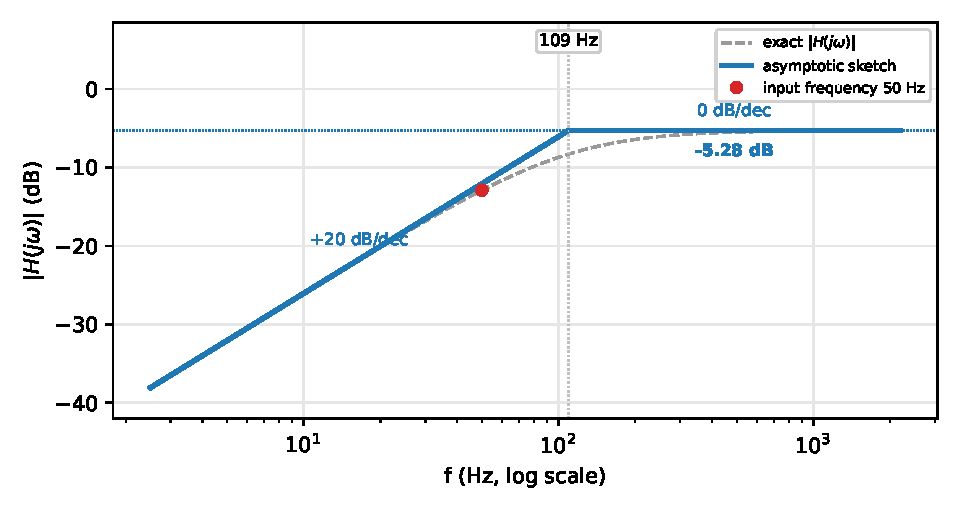
\includegraphics[width=0.78\linewidth,height=6.5cm,keepaspectratio]{p03_bode}\end{center}

{\small Blue: the straight-line sketch you are expected to draw. Dashed grey: the exact curve (about 3\,dB below the corner of an isolated pole). Red dot: the input frequency of Step 7.}
\solstep{7}{Steady-state output}The input is $V_i(t) = 0.5\sin\left(2\pi\cdot 50\,t\right)$, so $\omega_{in} = 2\pi\cdot 50 = 314$\,rad/s. Put $s=j\omega_{in}$ in each factor (tool T5): magnitudes multiply, angles add.
{\small Rules: $\left|\frac{s}{s+p}\right| = \frac{\omega}{\sqrt{\omega^2+p^2}}$, $\angle = \frac{\pi}{2}-\tan^{-1}\frac{\omega}{p}$;\quad $\left|\frac{1}{1+s/p}\right| = \frac{1}{\sqrt{1+(\omega/p)^2}}$, $\angle = -\tan^{-1}\frac{\omega}{p}$;\quad $\left|1+\frac{s}{z}\right| = \sqrt{1+(\omega/z)^2}$, $\angle = \tan^{-1}\frac{\omega}{z}$;\quad a negative $K$ adds $-\pi$.}
\begin{center}\renewcommand{\arraystretch}{1.35}
\begin{tabular}{ccc}
\toprule
factor & magnitude & angle (rad) \\
\midrule
$0.544$ & $0.5444$ & $0$ \\
$\rule[-1.1em]{0pt}{2.8em}\dfrac{s}{s+2\pi\cdot 109}$ & $0.416$ & $1.14$ \\
\textbf{total} & $\mathbf{0.2265}$ (product) & $\mathbf{1.14}$ (sum) \\
\bottomrule
\end{tabular}\end{center}

\begin{align*}
|H(j\omega_{in})| &= 0.226, \qquad \angle H(j\omega_{in}) = 1.14\ \mathrm{rad} \\
v_{o,ac}(t) &= 0.226\times 0.5\,\sin\left(2\pi\cdot 50\,t + 1.14\right) = 0.113\,\sin\left(2\pi\cdot 50\,t + 1.14\right)
\end{align*}

\[
\boxed{V_o(t) = 0.113\,\sin\left(2\pi\cdot 50\,t + 1.14\right)\ \mathrm{V}}
\]

\begin{ansbox}
$H(s) = 0.544\,\dfrac{s}{s+2\pi\cdot 109}$\quad (corners: 109 Hz)\\[4pt]
$V_o(t) = 0.113\,\sin\left(2\pi\cdot 50\,t + 1.14\right)\ \mathrm{V}$
\end{ansbox}

\newpage
\subsection*{Solution 5D.4 \hfill Easy}
\begin{center}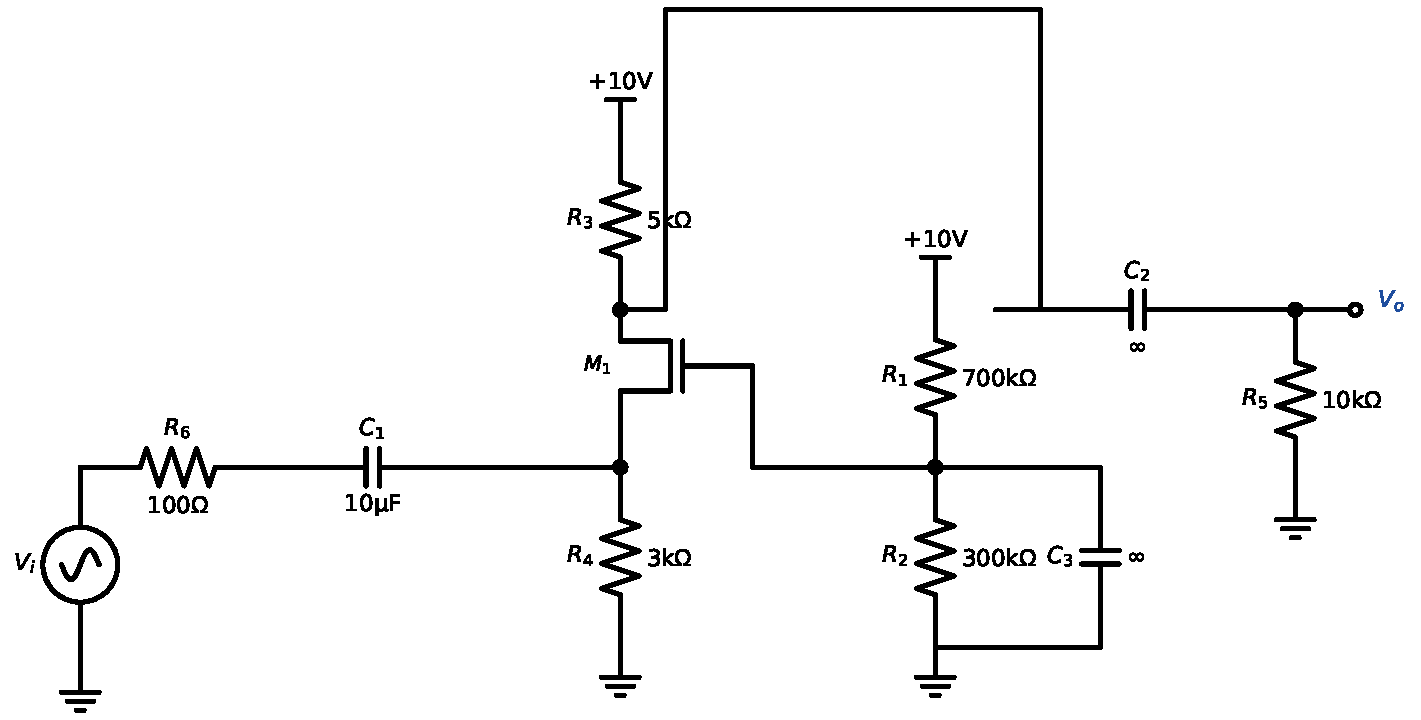
\includegraphics[width=0.9\linewidth,height=6cm,keepaspectratio]{p04_circuit}\end{center}
\solstep{1}{DC currents and transconductances}The DC drain currents are given: $I_{D1} = 444\,\mu \mathrm{A}$. For AC every DC supply is ground and every ``$\infty$'' capacitor is a short. Transconductances (tool T4):\begin{align*}
g_{m1} &= k_{1}V_{ov1} = \sqrt{2k_{1}I_{D1}} = \sqrt{2\cdot2\,\mathrm{m}\mathrm{A/V^2}\cdot444\,\mu \mathrm{A}} = 1.33\,\mathrm{m}\mathrm{A/V},\qquad \frac{1}{g_{m1}} = 750\,\Omega\quad(V_{ov1} = 0.667\,\mathrm{V})
\end{align*}

\solstep{2}{Input resistance of each stage}Input resistance of every stage, from the last back to the first (each one loads the stage before it):\begin{align*}
R_{i1} &= Z_{source,1} = \frac{1}{g_{m1}} = 750\,\Omega\quad\text{(common gate)}
\end{align*}

\solstep{3}{Gain along the signal path}Multiply the node-to-node gains along the signal path (tool T4):\[
H(s) = \frac{v_{s1}}{v_i}\cdot\frac{v_{d1}}{v_{s1}}
\]
\begin{align*}
\frac{v_{s1}}{v_i} &= \frac{R_{4} \parallel R_{i1}}{R_{6} + \frac{1}{sC_{1}} + R_{4} \parallel R_{i1}} = \dfrac{0.857\,s}{s + 143} \\
\frac{v_{d1}}{v_{s1}} &= \frac{Z_{D1}}{1/g_{m1}},\quad Z_{D1} = R_{3} \parallel R_{5}\ \Rightarrow\ 4.44
\end{align*}

\solstep{4}{Transfer function}Multiply and simplify:\[
H(s) = \dfrac{3.81\,s}{s + 143}
\]

\solstep{5}{Standard (Bode-ready) form}Find the roots. Every root $s=-p$ of the denominator is a \emph{pole}, every root $s=-z$ of the numerator is a \emph{zero}; $|p|$ and $|z|$ are the corner frequencies (rad/s).
\begin{itemize}[leftmargin=*,itemsep=2pt]
\item Numerator: it has the factor $s$ $\Rightarrow$ 1 zero at $s=0$.
\item Denominator: $s + 143$; $s + 143 = 0 \Rightarrow s = -143$.
\end{itemize}

Factored form (leading coefficient in front):
\[
H(s) = 3.81\,\dfrac{s}{(s+143)}
\]

Bode-ready form: rewrite every $(s+p) = p\left(1+\frac{s}{p}\right)$ and $(s+z) = z\left(1+\frac{s}{z}\right)$, and collect all constants into $K$. Each $s$ in the numerator is paired with one of the \emph{lowest} poles as $\frac{s}{s+p}$ (that factor is $\approx 1$ above $p$). Then every factor except $K$ is $\approx 1$ inside the pass-band:
\[
H(s) = 3.81\,\dfrac{s}{s+2\pi\cdot 22.7},\qquad K = 3.81
\]

\begin{center}\renewcommand{\arraystretch}{1.35}
\begin{tabular}{cccc}
\toprule
type & $\omega_c$ (rad/s) & $f_c=\omega_c/2\pi$ & slope change \\
\midrule
pole & $143$ & 22.7 Hz & $-20$ dB/dec \\
\bottomrule
\end{tabular}\end{center}

\solstep{6}{Magnitude Bode plot}Below every corner $|H(s)|\approx 0.0267\,s$, so the plot starts with a slope of $+20$\,dB/dec. Then, moving right, each pole bends the line down by 20\,dB/dec and each zero bends it up by 20\,dB/dec (tool T6):
\begin{center}\renewcommand{\arraystretch}{1.35}
\begin{tabular}{lcl}
\toprule
frequency range & slope & asymptote level \\
\midrule
$f<$ 22.7 Hz & $+20$ dB/dec & 11.6 dB at end \\
$f>$ 22.7 Hz & $0$ dB/dec (flat) & 11.6 dB at start \\
\bottomrule
\end{tabular}\end{center}

The flat (pass-band) level is $20\log_{10}|K| = 20\log_{10}3.81 = 11.6$\,dB.
\begin{center}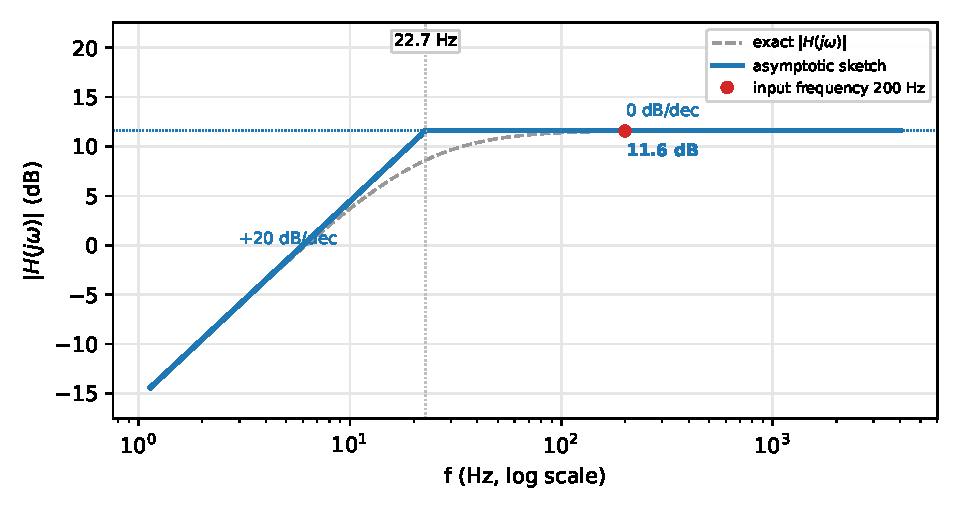
\includegraphics[width=0.78\linewidth,height=6.5cm,keepaspectratio]{p04_bode}\end{center}

{\small Blue: the straight-line sketch you are expected to draw. Dashed grey: the exact curve (about 3\,dB below the corner of an isolated pole). Red dot: the input frequency of Step 7.}
\solstep{7}{Steady-state output}The input is $V_i(t) = 0.005\sin\left(2\pi\cdot 200\,t\right)$, so $\omega_{in} = 2\pi\cdot 200 = 1260$\,rad/s. Put $s=j\omega_{in}$ in each factor (tool T5): magnitudes multiply, angles add.
{\small Rules: $\left|\frac{s}{s+p}\right| = \frac{\omega}{\sqrt{\omega^2+p^2}}$, $\angle = \frac{\pi}{2}-\tan^{-1}\frac{\omega}{p}$;\quad $\left|\frac{1}{1+s/p}\right| = \frac{1}{\sqrt{1+(\omega/p)^2}}$, $\angle = -\tan^{-1}\frac{\omega}{p}$;\quad $\left|1+\frac{s}{z}\right| = \sqrt{1+(\omega/z)^2}$, $\angle = \tan^{-1}\frac{\omega}{z}$;\quad a negative $K$ adds $-\pi$.}
\begin{center}\renewcommand{\arraystretch}{1.35}
\begin{tabular}{ccc}
\toprule
factor & magnitude & angle (rad) \\
\midrule
$3.81$ & $3.81$ & $0$ \\
$\rule[-1.1em]{0pt}{2.8em}\dfrac{s}{s+2\pi\cdot 22.7}$ & $0.9936$ & $0.113$ \\
\textbf{total} & $\mathbf{3.785}$ (product) & $\mathbf{0.113}$ (sum) \\
\bottomrule
\end{tabular}\end{center}

\begin{align*}
|H(j\omega_{in})| &= 3.79, \qquad \angle H(j\omega_{in}) = 0.113\ \mathrm{rad} \\
v_{o,ac}(t) &= 3.79\times 0.005\,\sin\left(2\pi\cdot 200\,t + 0.113\right) = 0.0189\,\sin\left(2\pi\cdot 200\,t + 0.113\right)
\end{align*}

\[
\boxed{V_o(t) = 0.0189\,\sin\left(2\pi\cdot 200\,t + 0.113\right)\ \mathrm{V}}
\]

\begin{ansbox}
$H(s) = 3.81\,\dfrac{s}{s+2\pi\cdot 22.7}$\quad (corners: 22.7 Hz)\\[4pt]
$V_o(t) = 0.0189\,\sin\left(2\pi\cdot 200\,t + 0.113\right)\ \mathrm{V}$
\end{ansbox}

\newpage
\subsection*{Solution 5D.5 \hfill Easy}
\begin{center}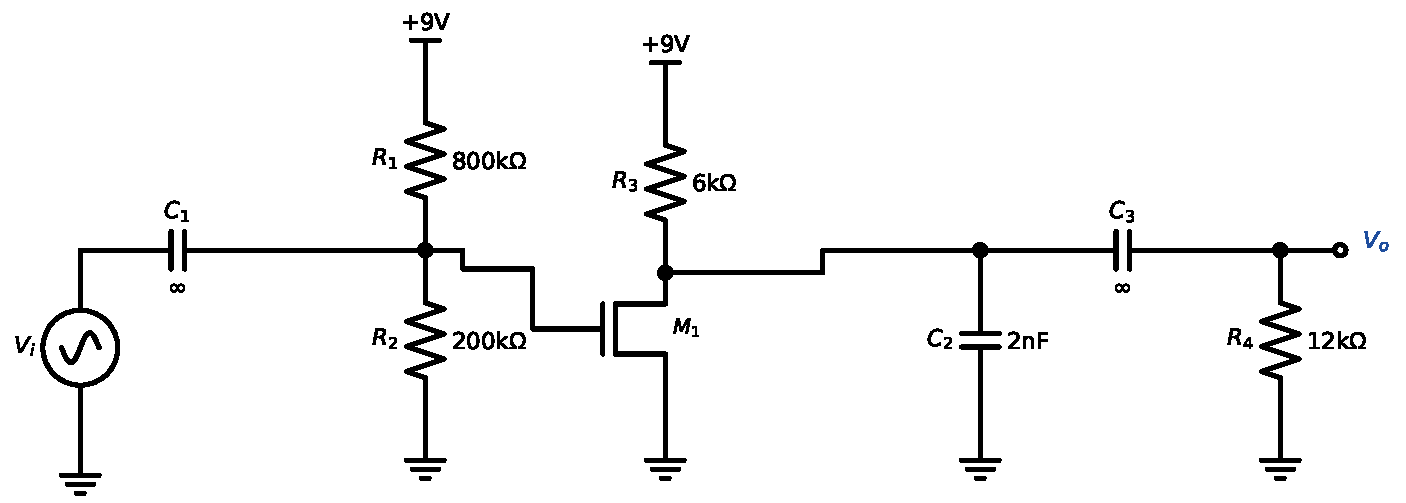
\includegraphics[width=0.9\linewidth,height=6cm,keepaspectratio]{p05_circuit}\end{center}
\solstep{1}{DC currents and transconductances}The DC drain currents are given: $I_{D1} = 640\,\mu \mathrm{A}$. For AC every DC supply is ground and every ``$\infty$'' capacitor is a short. Transconductances (tool T4):\begin{align*}
g_{m1} &= k_{1}V_{ov1} = \sqrt{2k_{1}I_{D1}} = \sqrt{2\cdot2\,\mathrm{m}\mathrm{A/V^2}\cdot640\,\mu \mathrm{A}} = 1.6\,\mathrm{m}\mathrm{A/V},\qquad \frac{1}{g_{m1}} = 625\,\Omega\quad(V_{ov1} = 0.8\,\mathrm{V})
\end{align*}

\solstep{2}{Input resistance of each stage}Input resistance of every stage, from the last back to the first (each one loads the stage before it):\begin{align*}
R_{i1} &= Z_{gate,1} = \infty\quad\text{(input at the gate: it loads nothing)}
\end{align*}

\solstep{3}{Gain along the signal path}Multiply the node-to-node gains along the signal path (tool T4):\[
H(s) = \frac{v_{d1}}{v_{g1}}
\]
\begin{align*}
\frac{v_{d1}}{v_{g1}} &= -\frac{Z_{D1}}{1/g_{m1} + Z_{S1}},\quad Z_{D1} = R_{3} \parallel \frac{1}{sC_{2}} \parallel R_{4},\ Z_{S1} = 0\ \Rightarrow\ \dfrac{-8\times 10^{5}}{s + 1.25\times 10^{5}}
\end{align*}

\solstep{4}{Transfer function}Multiply and simplify:\[
H(s) = \dfrac{-8\times 10^{5}}{s + 1.25\times 10^{5}}
\]

\solstep{5}{Standard (Bode-ready) form}Find the roots. Every root $s=-p$ of the denominator is a \emph{pole}, every root $s=-z$ of the numerator is a \emph{zero}; $|p|$ and $|z|$ are the corner frequencies (rad/s).
\begin{itemize}[leftmargin=*,itemsep=2pt]
\item Denominator: $s + 1.25\times 10^{5}$; $s + 1.25\times 10^{5} = 0 \Rightarrow s = -1.25\times 10^{5}$.
\end{itemize}

Factored form (leading coefficient in front):
\[
H(s) = -8\times 10^{5}\,\dfrac{1}{(s+1.25\times 10^{5})}
\]

Bode-ready form: rewrite every $(s+p) = p\left(1+\frac{s}{p}\right)$ and $(s+z) = z\left(1+\frac{s}{z}\right)$, and collect all constants into $K$. Then every factor except $K$ is $\approx 1$ inside the pass-band:
\[
H(s) = -6.4\,\dfrac{1}{1+\dfrac{s}{2\pi\cdot 19.9\mathrm{k}}},\qquad K = -6.4
\]

\begin{center}\renewcommand{\arraystretch}{1.35}
\begin{tabular}{cccc}
\toprule
type & $\omega_c$ (rad/s) & $f_c=\omega_c/2\pi$ & slope change \\
\midrule
pole & $1.25\times 10^{5}$ & 19.9 kHz & $-20$ dB/dec \\
\bottomrule
\end{tabular}\end{center}

\solstep{6}{Magnitude Bode plot}Below every corner, all factors are $\approx$ constant: $|H| \approx 6.4$ $= 16.1$\,dB (flat, 0 dB/dec). Then, moving right, each pole bends the line down by 20\,dB/dec and each zero bends it up by 20\,dB/dec (tool T6):
\begin{center}\renewcommand{\arraystretch}{1.35}
\begin{tabular}{lcl}
\toprule
frequency range & slope & asymptote level \\
\midrule
$f<$ 19.9 kHz & $0$ dB/dec (flat) & 16.1 dB at end \\
$f>$ 19.9 kHz & $-20$ dB/dec & 16.1 dB at start \\
\bottomrule
\end{tabular}\end{center}

The flat (pass-band) level is $20\log_{10}|K| = 20\log_{10}6.4 = 16.1$\,dB.
\begin{center}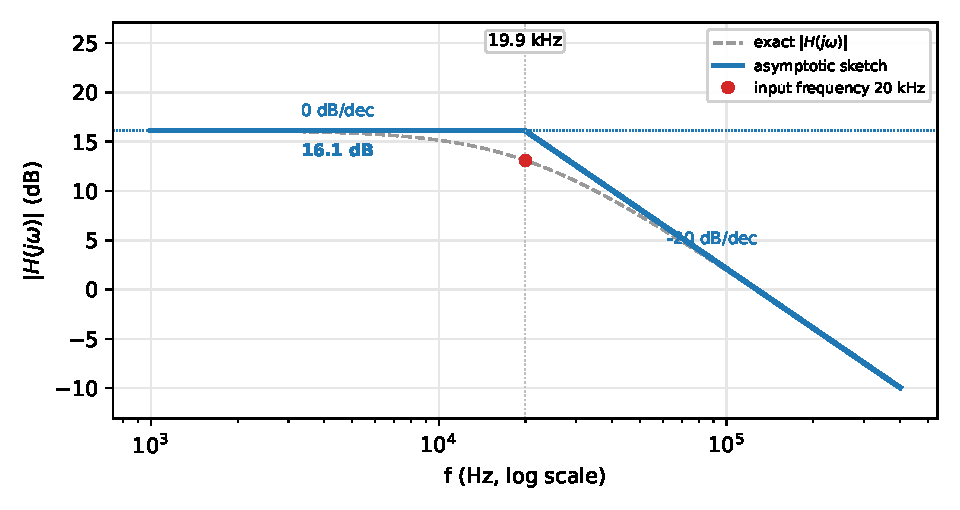
\includegraphics[width=0.78\linewidth,height=6.5cm,keepaspectratio]{p05_bode}\end{center}

{\small Blue: the straight-line sketch you are expected to draw. Dashed grey: the exact curve (about 3\,dB below the corner of an isolated pole). Red dot: the input frequency of Step 7.}
\solstep{7}{Steady-state output}The input is $V_i(t) = 0.01\sin\left(2\pi\cdot 20000\,t\right)$, so $\omega_{in} = 2\pi\cdot 20000 = 1.26\times 10^{5}$\,rad/s. Put $s=j\omega_{in}$ in each factor (tool T5): magnitudes multiply, angles add.
{\small Rules: $\left|\frac{s}{s+p}\right| = \frac{\omega}{\sqrt{\omega^2+p^2}}$, $\angle = \frac{\pi}{2}-\tan^{-1}\frac{\omega}{p}$;\quad $\left|\frac{1}{1+s/p}\right| = \frac{1}{\sqrt{1+(\omega/p)^2}}$, $\angle = -\tan^{-1}\frac{\omega}{p}$;\quad $\left|1+\frac{s}{z}\right| = \sqrt{1+(\omega/z)^2}$, $\angle = \tan^{-1}\frac{\omega}{z}$;\quad a negative $K$ adds $-\pi$.}
\begin{center}\renewcommand{\arraystretch}{1.35}
\begin{tabular}{ccc}
\toprule
factor & magnitude & angle (rad) \\
\midrule
$-6.4$ & $6.4$ & $-3.14$ \\
$\rule[-1.7em]{0pt}{4em}\dfrac{1}{1+\dfrac{s}{2\pi\cdot 19.9\mathrm{k}}}$ & $0.7052$ & $-0.788$ \\
\textbf{total} & $\mathbf{4.513}$ (product) & $\mathbf{-3.93}$ (sum) \\
\bottomrule
\end{tabular}\end{center}

\begin{align*}
|H(j\omega_{in})| &= 4.51, \qquad \angle H(j\omega_{in}) = -3.93\ \mathrm{rad} \\
v_{o,ac}(t) &= 4.51\times 0.01\,\sin\left(2\pi\cdot 20000\,t - 3.93\right) = 0.0451\,\sin\left(2\pi\cdot 20000\,t - 3.93\right)
\end{align*}

\[
\boxed{V_o(t) = 0.0451\,\sin\left(2\pi\cdot 20000\,t - 3.93\right)\ \mathrm{V}}
\]

\begin{ansbox}
$H(s) = -6.4\,\dfrac{1}{1+\dfrac{s}{2\pi\cdot 19.9\mathrm{k}}}$\quad (corners: 19.9 kHz)\\[4pt]
$V_o(t) = 0.0451\,\sin\left(2\pi\cdot 20000\,t - 3.93\right)\ \mathrm{V}$
\end{ansbox}

\newpage
\subsection*{Solution 5D.6 \hfill Easy}
\begin{center}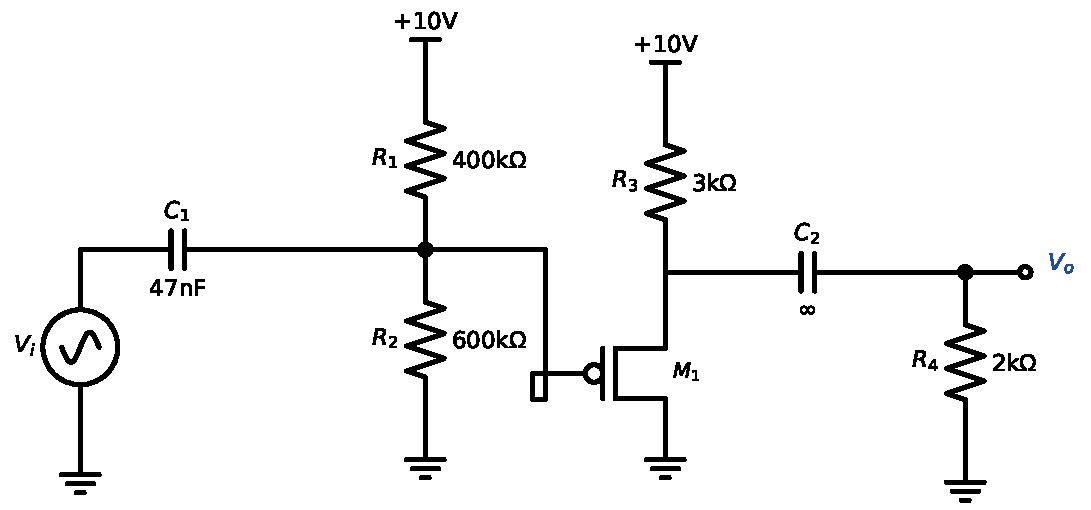
\includegraphics[width=0.9\linewidth,height=6cm,keepaspectratio]{p06_circuit}\end{center}
\solstep{1}{DC currents and transconductances}The DC drain currents are given: $I_{D1} = 528\,\mu \mathrm{A}$. For AC every DC supply is ground and every ``$\infty$'' capacitor is a short. Transconductances (tool T4):\begin{align*}
g_{m1} &= k_{1}V_{ov1} = \sqrt{2k_{1}I_{D1}} = \sqrt{2\cdot850\,\mu \mathrm{A/V^2}\cdot528\,\mu \mathrm{A}} = 948\,\mu \mathrm{A/V},\qquad \frac{1}{g_{m1}} = 1.06\,\mathrm{k}\Omega\quad(V_{ov1} = 1.11\,\mathrm{V})
\end{align*}

\solstep{2}{Input resistance of each stage}Input resistance of every stage, from the last back to the first (each one loads the stage before it):\begin{align*}
R_{i1} &= Z_{gate,1} = \infty\quad\text{(input at the gate: it loads nothing)}
\end{align*}

\solstep{3}{Gain along the signal path}Multiply the node-to-node gains along the signal path (tool T4):\[
H(s) = \frac{v_{g1}}{v_i}\cdot\frac{v_{s1}}{v_{g1}}
\]
\begin{align*}
\frac{v_{g1}}{v_i} &= \frac{R_{1} \parallel R_{2}}{\frac{1}{sC_{1}} + R_{1} \parallel R_{2}} = \dfrac{s}{s + 88.7} \\
\frac{v_{s1}}{v_{g1}} &= \frac{Z_{S1}}{1/g_{m1} + Z_{S1}},\quad Z_{S1} = R_{3} \parallel R_{4}\ \Rightarrow\ 0.532
\end{align*}

\solstep{4}{Transfer function}Multiply and simplify:\[
H(s) = \dfrac{0.532\,s}{s + 88.7}
\]

\solstep{5}{Standard (Bode-ready) form}Find the roots. Every root $s=-p$ of the denominator is a \emph{pole}, every root $s=-z$ of the numerator is a \emph{zero}; $|p|$ and $|z|$ are the corner frequencies (rad/s).
\begin{itemize}[leftmargin=*,itemsep=2pt]
\item Numerator: it has the factor $s$ $\Rightarrow$ 1 zero at $s=0$.
\item Denominator: $s + 88.7$; $s + 88.7 = 0 \Rightarrow s = -88.7$.
\end{itemize}

Factored form (leading coefficient in front):
\[
H(s) = 0.532\,\dfrac{s}{(s+88.7)}
\]

Bode-ready form: rewrite every $(s+p) = p\left(1+\frac{s}{p}\right)$ and $(s+z) = z\left(1+\frac{s}{z}\right)$, and collect all constants into $K$. Each $s$ in the numerator is paired with one of the \emph{lowest} poles as $\frac{s}{s+p}$ (that factor is $\approx 1$ above $p$). Then every factor except $K$ is $\approx 1$ inside the pass-band:
\[
H(s) = 0.532\,\dfrac{s}{s+2\pi\cdot 14.1},\qquad K = 0.532
\]

\begin{center}\renewcommand{\arraystretch}{1.35}
\begin{tabular}{cccc}
\toprule
type & $\omega_c$ (rad/s) & $f_c=\omega_c/2\pi$ & slope change \\
\midrule
pole & $88.7$ & 14.1 Hz & $-20$ dB/dec \\
\bottomrule
\end{tabular}\end{center}

\solstep{6}{Magnitude Bode plot}Below every corner $|H(s)|\approx 0.006\,s$, so the plot starts with a slope of $+20$\,dB/dec. Then, moving right, each pole bends the line down by 20\,dB/dec and each zero bends it up by 20\,dB/dec (tool T6):
\begin{center}\renewcommand{\arraystretch}{1.35}
\begin{tabular}{lcl}
\toprule
frequency range & slope & asymptote level \\
\midrule
$f<$ 14.1 Hz & $+20$ dB/dec & -5.48 dB at end \\
$f>$ 14.1 Hz & $0$ dB/dec (flat) & -5.48 dB at start \\
\bottomrule
\end{tabular}\end{center}

The flat (pass-band) level is $20\log_{10}|K| = 20\log_{10}0.532 = -5.48$\,dB.
\begin{center}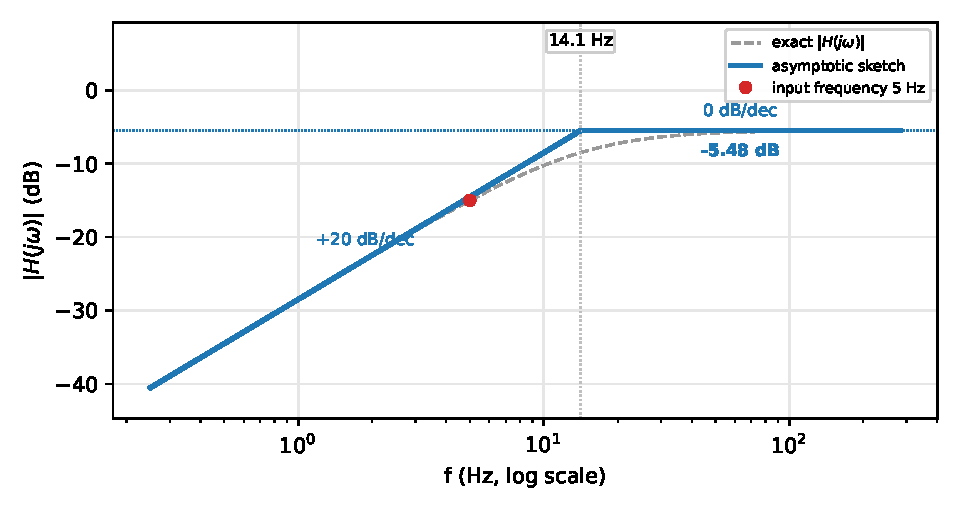
\includegraphics[width=0.78\linewidth,height=6.5cm,keepaspectratio]{p06_bode}\end{center}

{\small Blue: the straight-line sketch you are expected to draw. Dashed grey: the exact curve (about 3\,dB below the corner of an isolated pole). Red dot: the input frequency of Step 7.}
\solstep{7}{Steady-state output}The input is $V_i(t) = 0.2\sin\left(2\pi\cdot 5\,t\right)$, so $\omega_{in} = 2\pi\cdot 5 = 31.4$\,rad/s. Put $s=j\omega_{in}$ in each factor (tool T5): magnitudes multiply, angles add.
{\small Rules: $\left|\frac{s}{s+p}\right| = \frac{\omega}{\sqrt{\omega^2+p^2}}$, $\angle = \frac{\pi}{2}-\tan^{-1}\frac{\omega}{p}$;\quad $\left|\frac{1}{1+s/p}\right| = \frac{1}{\sqrt{1+(\omega/p)^2}}$, $\angle = -\tan^{-1}\frac{\omega}{p}$;\quad $\left|1+\frac{s}{z}\right| = \sqrt{1+(\omega/z)^2}$, $\angle = \tan^{-1}\frac{\omega}{z}$;\quad a negative $K$ adds $-\pi$.}
\begin{center}\renewcommand{\arraystretch}{1.35}
\begin{tabular}{ccc}
\toprule
factor & magnitude & angle (rad) \\
\midrule
$0.532$ & $0.5321$ & $0$ \\
$\rule[-1.1em]{0pt}{2.8em}\dfrac{s}{s+2\pi\cdot 14.1}$ & $0.334$ & $1.23$ \\
\textbf{total} & $\mathbf{0.1777}$ (product) & $\mathbf{1.23}$ (sum) \\
\bottomrule
\end{tabular}\end{center}

\begin{align*}
|H(j\omega_{in})| &= 0.178, \qquad \angle H(j\omega_{in}) = 1.23\ \mathrm{rad} \\
v_{o,ac}(t) &= 0.178\times 0.2\,\sin\left(2\pi\cdot 5\,t + 1.23\right) = 0.0355\,\sin\left(2\pi\cdot 5\,t + 1.23\right)
\end{align*}

\[
\boxed{V_o(t) = 0.0355\,\sin\left(2\pi\cdot 5\,t + 1.23\right)\ \mathrm{V}}
\]

\begin{ansbox}
$H(s) = 0.532\,\dfrac{s}{s+2\pi\cdot 14.1}$\quad (corners: 14.1 Hz)\\[4pt]
$V_o(t) = 0.0355\,\sin\left(2\pi\cdot 5\,t + 1.23\right)\ \mathrm{V}$
\end{ansbox}

\newpage
\subsection*{Solution 5D.7 \hfill Medium}
\begin{center}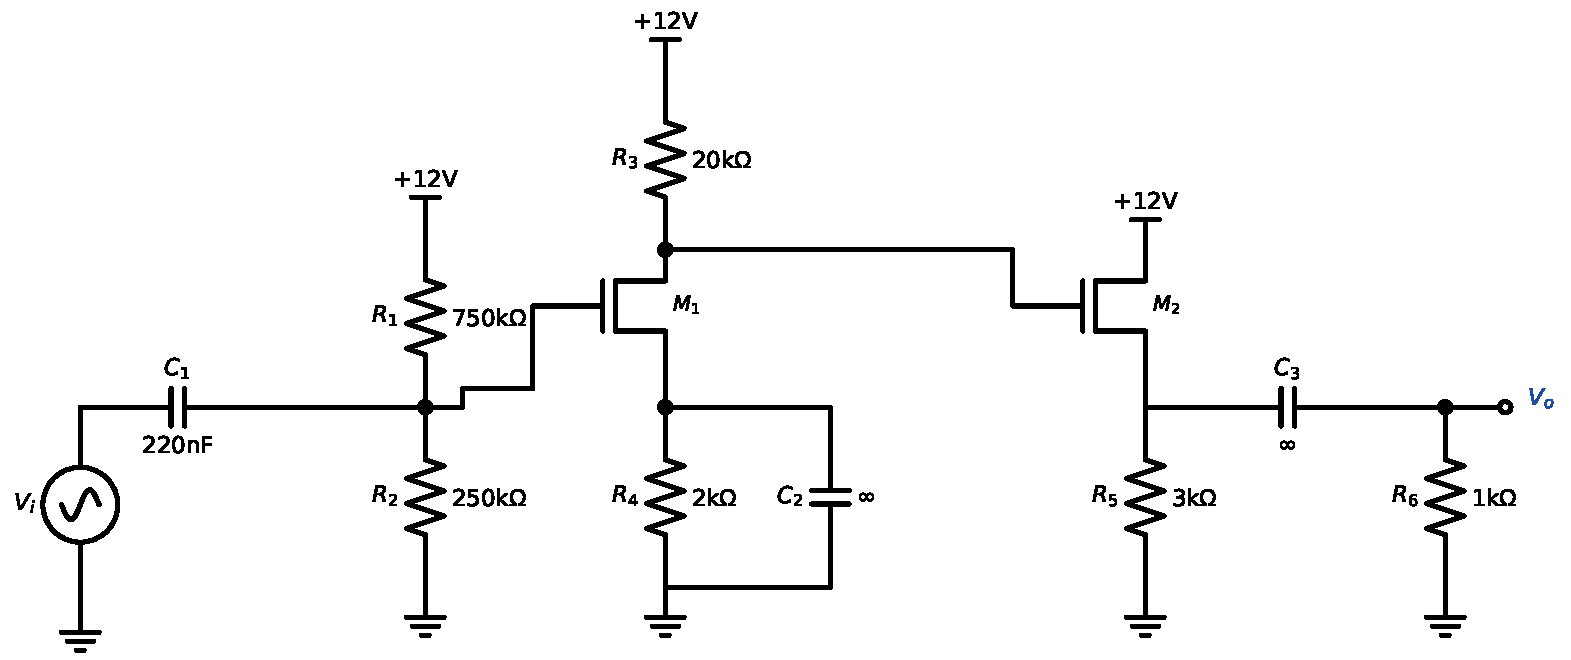
\includegraphics[width=0.9\linewidth,height=6cm,keepaspectratio]{p07_circuit}\end{center}
\solstep{1}{DC currents and transconductances}The DC drain currents are given: $I_{D1} = 383\,\mu \mathrm{A}$, $I_{D2} = 626\,\mu \mathrm{A}$. For AC every DC supply is ground and every ``$\infty$'' capacitor is a short. Transconductances (tool T4):\begin{align*}
g_{m1} &= k_{1}V_{ov1} = \sqrt{2k_{1}I_{D1}} = \sqrt{2\cdot1.1\,\mathrm{m}\mathrm{A/V^2}\cdot383\,\mu \mathrm{A}} = 918\,\mu \mathrm{A/V},\qquad \frac{1}{g_{m1}} = 1.09\,\mathrm{k}\Omega\quad(V_{ov1} = 0.834\,\mathrm{V}) \\
g_{m2} &= k_{2}V_{ov2} = \sqrt{2k_{2}I_{D2}} = \sqrt{2\cdot1.1\,\mathrm{m}\mathrm{A/V^2}\cdot626\,\mu \mathrm{A}} = 1.17\,\mathrm{m}\mathrm{A/V},\qquad \frac{1}{g_{m2}} = 852\,\Omega\quad(V_{ov2} = 1.07\,\mathrm{V})
\end{align*}

\solstep{2}{Input resistance of each stage}Input resistance of every stage, from the last back to the first (each one loads the stage before it):\begin{align*}
R_{i1} &= Z_{gate,1} = \infty\quad\text{(input at the gate: it loads nothing)} \\
R_{i2} &= Z_{gate,2} = \infty\quad\text{(input at the gate: it loads nothing)}
\end{align*}

\solstep{3}{Gain along the signal path}Multiply the node-to-node gains along the signal path (tool T4):\[
H(s) = \frac{v_{g1}}{v_i}\cdot\frac{v_{d1}}{v_{g1}}\cdot\frac{v_{s2}}{v_{g2}}
\]
\begin{align*}
\frac{v_{g1}}{v_i} &= \frac{R_{1} \parallel R_{2}}{\frac{1}{sC_{1}} + R_{1} \parallel R_{2}} = \dfrac{s}{s + 24.2} \\
\frac{v_{d1}}{v_{g1}} &= -\frac{Z_{D1}}{1/g_{m1} + Z_{S1}},\quad Z_{D1} = R_{3},\ Z_{S1} = 0\ \Rightarrow\ -18.4 \\
\frac{v_{s2}}{v_{g2}} &= \frac{Z_{S2}}{1/g_{m2} + Z_{S2}},\quad Z_{S2} = R_{5} \parallel R_{6}\ \Rightarrow\ 0.468
\end{align*}

\solstep{4}{Transfer function}Multiply and simplify:\[
H(s) = \dfrac{-8.59\,s}{s + 24.2}
\]

\solstep{5}{Standard (Bode-ready) form}Find the roots. Every root $s=-p$ of the denominator is a \emph{pole}, every root $s=-z$ of the numerator is a \emph{zero}; $|p|$ and $|z|$ are the corner frequencies (rad/s).
\begin{itemize}[leftmargin=*,itemsep=2pt]
\item Numerator: it has the factor $s$ $\Rightarrow$ 1 zero at $s=0$.
\item Denominator: $s + 24.2$; $s + 24.2 = 0 \Rightarrow s = -24.2$.
\end{itemize}

Factored form (leading coefficient in front):
\[
H(s) = -8.59\,\dfrac{s}{(s+24.2)}
\]

Bode-ready form: rewrite every $(s+p) = p\left(1+\frac{s}{p}\right)$ and $(s+z) = z\left(1+\frac{s}{z}\right)$, and collect all constants into $K$. Each $s$ in the numerator is paired with one of the \emph{lowest} poles as $\frac{s}{s+p}$ (that factor is $\approx 1$ above $p$). Then every factor except $K$ is $\approx 1$ inside the pass-band:
\[
H(s) = -8.59\,\dfrac{s}{s+2\pi\cdot 3.86},\qquad K = -8.59
\]

\begin{center}\renewcommand{\arraystretch}{1.35}
\begin{tabular}{cccc}
\toprule
type & $\omega_c$ (rad/s) & $f_c=\omega_c/2\pi$ & slope change \\
\midrule
pole & $24.2$ & 3.86 Hz & $-20$ dB/dec \\
\bottomrule
\end{tabular}\end{center}

\solstep{6}{Magnitude Bode plot}Below every corner $|H(s)|\approx 0.354\,s$, so the plot starts with a slope of $+20$\,dB/dec. Then, moving right, each pole bends the line down by 20\,dB/dec and each zero bends it up by 20\,dB/dec (tool T6):
\begin{center}\renewcommand{\arraystretch}{1.35}
\begin{tabular}{lcl}
\toprule
frequency range & slope & asymptote level \\
\midrule
$f<$ 3.86 Hz & $+20$ dB/dec & 18.7 dB at end \\
$f>$ 3.86 Hz & $0$ dB/dec (flat) & 18.7 dB at start \\
\bottomrule
\end{tabular}\end{center}

The flat (pass-band) level is $20\log_{10}|K| = 20\log_{10}8.59 = 18.7$\,dB.
\begin{center}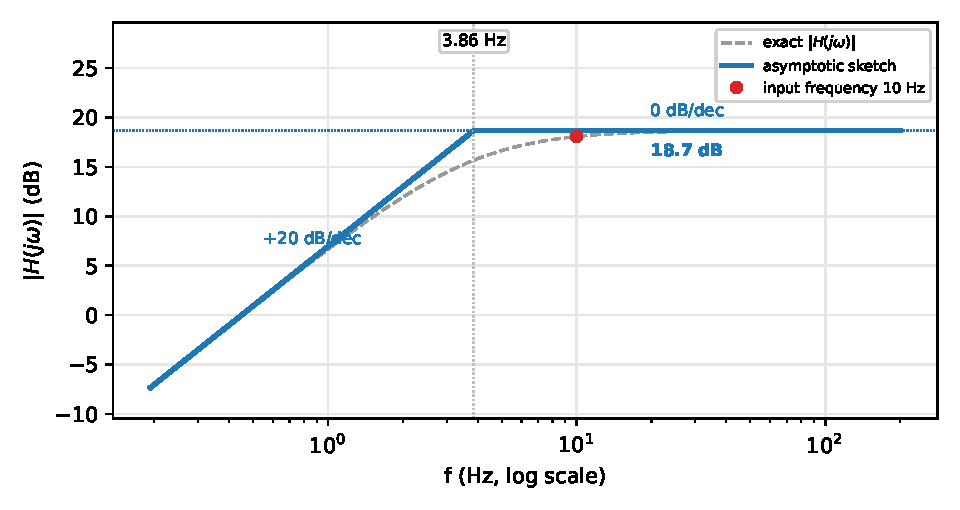
\includegraphics[width=0.78\linewidth,height=6.5cm,keepaspectratio]{p07_bode}\end{center}

{\small Blue: the straight-line sketch you are expected to draw. Dashed grey: the exact curve (about 3\,dB below the corner of an isolated pole). Red dot: the input frequency of Step 7.}
\solstep{7}{Steady-state output}The input is $V_i(t) = 0.005\sin\left(2\pi\cdot 10\,t\right)$, so $\omega_{in} = 2\pi\cdot 10 = 62.8$\,rad/s. Put $s=j\omega_{in}$ in each factor (tool T5): magnitudes multiply, angles add.
{\small Rules: $\left|\frac{s}{s+p}\right| = \frac{\omega}{\sqrt{\omega^2+p^2}}$, $\angle = \frac{\pi}{2}-\tan^{-1}\frac{\omega}{p}$;\quad $\left|\frac{1}{1+s/p}\right| = \frac{1}{\sqrt{1+(\omega/p)^2}}$, $\angle = -\tan^{-1}\frac{\omega}{p}$;\quad $\left|1+\frac{s}{z}\right| = \sqrt{1+(\omega/z)^2}$, $\angle = \tan^{-1}\frac{\omega}{z}$;\quad a negative $K$ adds $-\pi$.}
\begin{center}\renewcommand{\arraystretch}{1.35}
\begin{tabular}{ccc}
\toprule
factor & magnitude & angle (rad) \\
\midrule
$-8.59$ & $8.591$ & $-3.14$ \\
$\rule[-1.1em]{0pt}{2.8em}\dfrac{s}{s+2\pi\cdot 3.86}$ & $0.933$ & $0.368$ \\
\textbf{total} & $\mathbf{8.015}$ (product) & $\mathbf{-2.77}$ (sum) \\
\bottomrule
\end{tabular}\end{center}

\begin{align*}
|H(j\omega_{in})| &= 8.01, \qquad \angle H(j\omega_{in}) = -2.77\ \mathrm{rad} \\
v_{o,ac}(t) &= 8.01\times 0.005\,\sin\left(2\pi\cdot 10\,t - 2.77\right) = 0.0401\,\sin\left(2\pi\cdot 10\,t - 2.77\right)
\end{align*}

\[
\boxed{V_o(t) = 0.0401\,\sin\left(2\pi\cdot 10\,t - 2.77\right)\ \mathrm{V}}
\]

\begin{ansbox}
$H(s) = -8.59\,\dfrac{s}{s+2\pi\cdot 3.86}$\quad (corners: 3.86 Hz)\\[4pt]
$V_o(t) = 0.0401\,\sin\left(2\pi\cdot 10\,t - 2.77\right)\ \mathrm{V}$
\end{ansbox}

\newpage
\subsection*{Solution 5D.8 \hfill Medium}
\begin{center}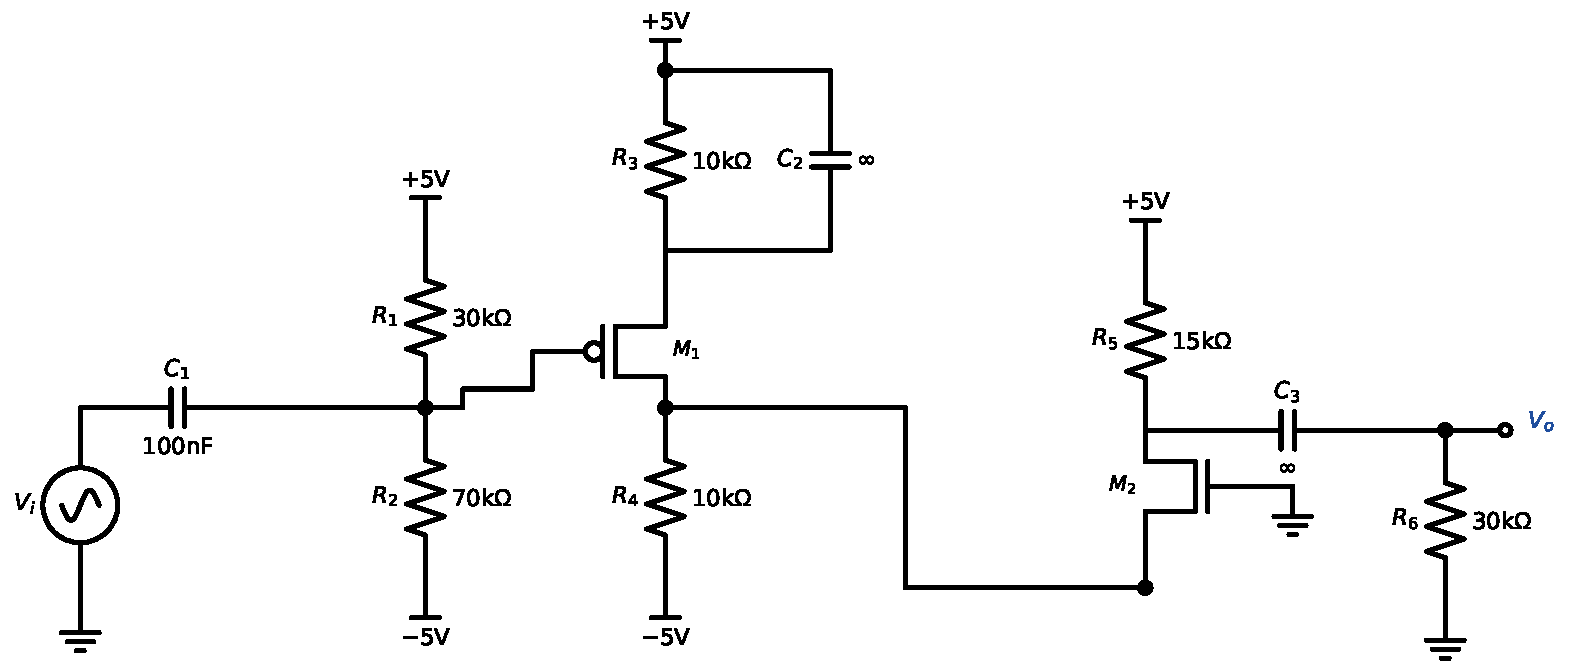
\includegraphics[width=0.9\linewidth,height=6cm,keepaspectratio]{p08_circuit}\end{center}
\solstep{1}{DC currents and transconductances}The DC drain currents are given: $I_{D1} = 117\,\mu \mathrm{A}$, $I_{D2} = 185\,\mu \mathrm{A}$. For AC every DC supply is ground and every ``$\infty$'' capacitor is a short. Transconductances (tool T4):\begin{align*}
g_{m1} &= k_{1}V_{ov1} = \sqrt{2k_{1}I_{D1}} = \sqrt{2\cdot850\,\mu \mathrm{A/V^2}\cdot117\,\mu \mathrm{A}} = 447\,\mu \mathrm{A/V},\qquad \frac{1}{g_{m1}} = 2.24\,\mathrm{k}\Omega\quad(V_{ov1} = 0.526\,\mathrm{V}) \\
g_{m2} &= k_{2}V_{ov2} = \sqrt{2k_{2}I_{D2}} = \sqrt{2\cdot1.1\,\mathrm{m}\mathrm{A/V^2}\cdot185\,\mu \mathrm{A}} = 637\,\mu \mathrm{A/V},\qquad \frac{1}{g_{m2}} = 1.57\,\mathrm{k}\Omega\quad(V_{ov2} = 0.579\,\mathrm{V})
\end{align*}

\solstep{2}{Input resistance of each stage}Input resistance of every stage, from the last back to the first (each one loads the stage before it):\begin{align*}
R_{i1} &= Z_{gate,1} = \infty\quad\text{(input at the gate: it loads nothing)} \\
R_{i2} &= Z_{source,2} = \frac{1}{g_{m2}} = 1.57\,\mathrm{k}\Omega\quad\text{(common gate)}
\end{align*}

\solstep{3}{Gain along the signal path}Multiply the node-to-node gains along the signal path (tool T4):\[
H(s) = \frac{v_{g1}}{v_i}\cdot\frac{v_{d1}}{v_{g1}}\cdot\frac{v_{d2}}{v_{s2}}
\]
\begin{align*}
\frac{v_{g1}}{v_i} &= \frac{R_{1} \parallel R_{2}}{\frac{1}{sC_{1}} + R_{1} \parallel R_{2}} = \dfrac{s}{s + 476} \\
\frac{v_{d1}}{v_{g1}} &= -\frac{Z_{D1}}{1/g_{m1} + Z_{S1}},\quad Z_{D1} = R_{4} \parallel R_{i2},\ Z_{S1} = 0\ \Rightarrow\ -0.606 \\
\frac{v_{d2}}{v_{s2}} &= \frac{Z_{D2}}{1/g_{m2}},\quad Z_{D2} = R_{5} \parallel R_{6}\ \Rightarrow\ 6.37
\end{align*}

\solstep{4}{Transfer function}Multiply and simplify:\[
H(s) = \dfrac{-3.86\,s}{s + 476}
\]

\solstep{5}{Standard (Bode-ready) form}Find the roots. Every root $s=-p$ of the denominator is a \emph{pole}, every root $s=-z$ of the numerator is a \emph{zero}; $|p|$ and $|z|$ are the corner frequencies (rad/s).
\begin{itemize}[leftmargin=*,itemsep=2pt]
\item Numerator: it has the factor $s$ $\Rightarrow$ 1 zero at $s=0$.
\item Denominator: $s + 476$; $s + 476 = 0 \Rightarrow s = -476$.
\end{itemize}

Factored form (leading coefficient in front):
\[
H(s) = -3.86\,\dfrac{s}{(s+476)}
\]

Bode-ready form: rewrite every $(s+p) = p\left(1+\frac{s}{p}\right)$ and $(s+z) = z\left(1+\frac{s}{z}\right)$, and collect all constants into $K$. Each $s$ in the numerator is paired with one of the \emph{lowest} poles as $\frac{s}{s+p}$ (that factor is $\approx 1$ above $p$). Then every factor except $K$ is $\approx 1$ inside the pass-band:
\[
H(s) = -3.86\,\dfrac{s}{s+2\pi\cdot 75.8},\qquad K = -3.86
\]

\begin{center}\renewcommand{\arraystretch}{1.35}
\begin{tabular}{cccc}
\toprule
type & $\omega_c$ (rad/s) & $f_c=\omega_c/2\pi$ & slope change \\
\midrule
pole & $476$ & 75.8 Hz & $-20$ dB/dec \\
\bottomrule
\end{tabular}\end{center}

\solstep{6}{Magnitude Bode plot}Below every corner $|H(s)|\approx 0.00811\,s$, so the plot starts with a slope of $+20$\,dB/dec. Then, moving right, each pole bends the line down by 20\,dB/dec and each zero bends it up by 20\,dB/dec (tool T6):
\begin{center}\renewcommand{\arraystretch}{1.35}
\begin{tabular}{lcl}
\toprule
frequency range & slope & asymptote level \\
\midrule
$f<$ 75.8 Hz & $+20$ dB/dec & 11.7 dB at end \\
$f>$ 75.8 Hz & $0$ dB/dec (flat) & 11.7 dB at start \\
\bottomrule
\end{tabular}\end{center}

The flat (pass-band) level is $20\log_{10}|K| = 20\log_{10}3.86 = 11.7$\,dB.
\begin{center}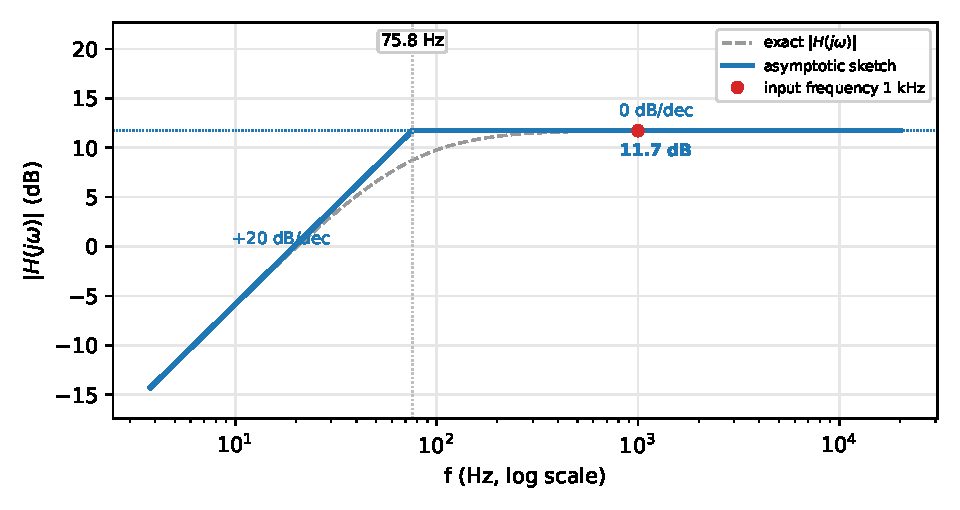
\includegraphics[width=0.78\linewidth,height=6.5cm,keepaspectratio]{p08_bode}\end{center}

{\small Blue: the straight-line sketch you are expected to draw. Dashed grey: the exact curve (about 3\,dB below the corner of an isolated pole). Red dot: the input frequency of Step 7.}
\solstep{7}{Steady-state output}The input is $V_i(t) = 0.005\sin\left(2\pi\cdot 1000\,t\right)$, so $\omega_{in} = 2\pi\cdot 1000 = 6280$\,rad/s. Put $s=j\omega_{in}$ in each factor (tool T5): magnitudes multiply, angles add.
{\small Rules: $\left|\frac{s}{s+p}\right| = \frac{\omega}{\sqrt{\omega^2+p^2}}$, $\angle = \frac{\pi}{2}-\tan^{-1}\frac{\omega}{p}$;\quad $\left|\frac{1}{1+s/p}\right| = \frac{1}{\sqrt{1+(\omega/p)^2}}$, $\angle = -\tan^{-1}\frac{\omega}{p}$;\quad $\left|1+\frac{s}{z}\right| = \sqrt{1+(\omega/z)^2}$, $\angle = \tan^{-1}\frac{\omega}{z}$;\quad a negative $K$ adds $-\pi$.}
\begin{center}\renewcommand{\arraystretch}{1.35}
\begin{tabular}{ccc}
\toprule
factor & magnitude & angle (rad) \\
\midrule
$-3.86$ & $3.862$ & $-3.14$ \\
$\rule[-1.1em]{0pt}{2.8em}\dfrac{s}{s+2\pi\cdot 75.8}$ & $0.9971$ & $0.0756$ \\
\textbf{total} & $\mathbf{3.851}$ (product) & $\mathbf{-3.07}$ (sum) \\
\bottomrule
\end{tabular}\end{center}

\begin{align*}
|H(j\omega_{in})| &= 3.85, \qquad \angle H(j\omega_{in}) = -3.07\ \mathrm{rad} \\
v_{o,ac}(t) &= 3.85\times 0.005\,\sin\left(2\pi\cdot 1000\,t - 3.07\right) = 0.0193\,\sin\left(2\pi\cdot 1000\,t - 3.07\right)
\end{align*}

\[
\boxed{V_o(t) = 0.0193\,\sin\left(2\pi\cdot 1000\,t - 3.07\right)\ \mathrm{V}}
\]

\begin{ansbox}
$H(s) = -3.86\,\dfrac{s}{s+2\pi\cdot 75.8}$\quad (corners: 75.8 Hz)\\[4pt]
$V_o(t) = 0.0193\,\sin\left(2\pi\cdot 1000\,t - 3.07\right)\ \mathrm{V}$
\end{ansbox}

\newpage
\subsection*{Solution 5D.9 \hfill Medium}
\begin{center}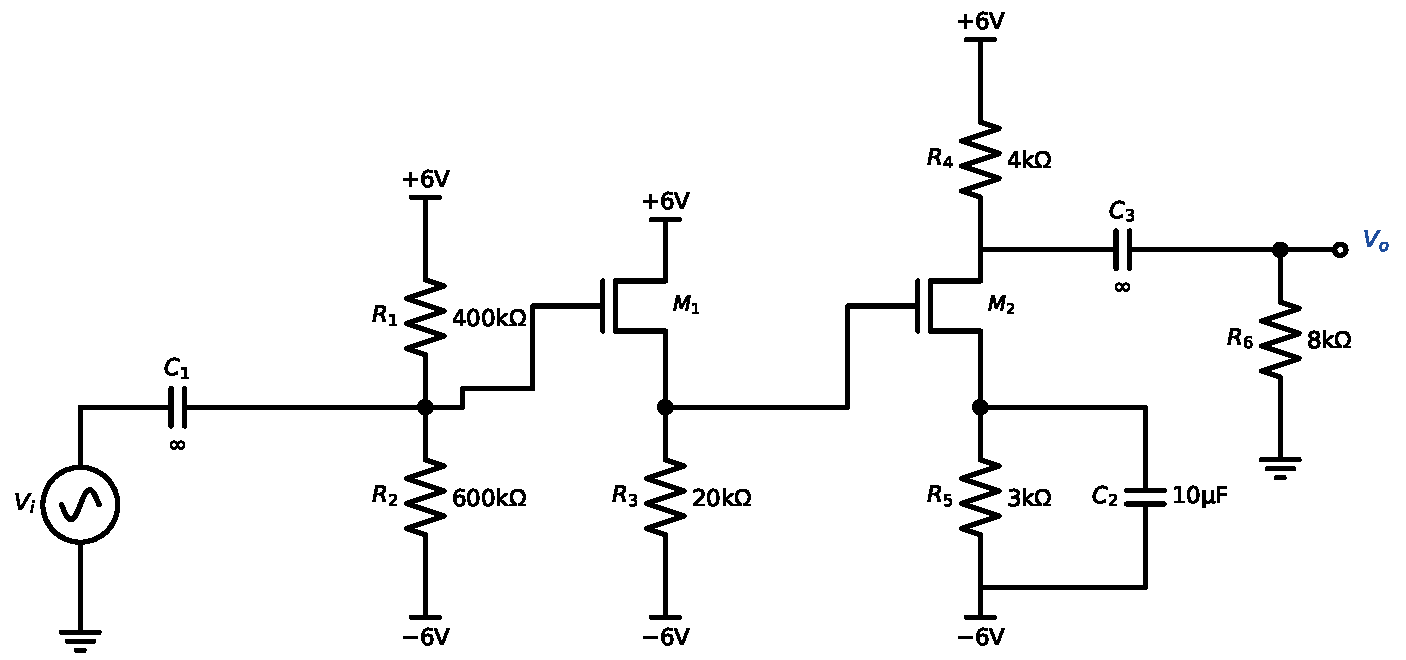
\includegraphics[width=0.9\linewidth,height=6cm,keepaspectratio]{p09_circuit}\end{center}
\solstep{1}{DC currents and transconductances}The DC drain currents are given: $I_{D1} = 256\,\mu \mathrm{A}$, $I_{D2} = 830\,\mu \mathrm{A}$. For AC every DC supply is ground and every ``$\infty$'' capacitor is a short. Transconductances (tool T4):\begin{align*}
g_{m1} &= k_{1}V_{ov1} = \sqrt{2k_{1}I_{D1}} = \sqrt{2\cdot1.1\,\mathrm{m}\mathrm{A/V^2}\cdot256\,\mu \mathrm{A}} = 750\,\mu \mathrm{A/V},\qquad \frac{1}{g_{m1}} = 1.33\,\mathrm{k}\Omega\quad(V_{ov1} = 0.682\,\mathrm{V}) \\
g_{m2} &= k_{2}V_{ov2} = \sqrt{2k_{2}I_{D2}} = \sqrt{2\cdot1.1\,\mathrm{m}\mathrm{A/V^2}\cdot830\,\mu \mathrm{A}} = 1.35\,\mathrm{m}\mathrm{A/V},\qquad \frac{1}{g_{m2}} = 740\,\Omega\quad(V_{ov2} = 1.23\,\mathrm{V})
\end{align*}

\solstep{2}{Input resistance of each stage}Input resistance of every stage, from the last back to the first (each one loads the stage before it):\begin{align*}
R_{i1} &= Z_{gate,1} = \infty\quad\text{(input at the gate: it loads nothing)} \\
R_{i2} &= Z_{gate,2} = \infty\quad\text{(input at the gate: it loads nothing)}
\end{align*}

\solstep{3}{Gain along the signal path}Multiply the node-to-node gains along the signal path (tool T4):\[
H(s) = \frac{v_{s1}}{v_{g1}}\cdot\frac{v_{d2}}{v_{g2}}
\]
\begin{align*}
\frac{v_{s1}}{v_{g1}} &= \frac{Z_{S1}}{1/g_{m1} + Z_{S1}},\quad Z_{S1} = R_{3}\ \Rightarrow\ 0.938 \\
\frac{v_{d2}}{v_{g2}} &= -\frac{Z_{D2}}{1/g_{m2} + Z_{S2}},\quad Z_{D2} = R_{4} \parallel R_{6},\ Z_{S2} = R_{5} \parallel \frac{1}{sC_{2}}\ \Rightarrow\ \dfrac{-3.6\,s - 120}{s + 168}
\end{align*}

\solstep{4}{Transfer function}Multiply and simplify:\[
H(s) = \dfrac{-3.38\,s - 113}{s + 168}
\]

\solstep{5}{Standard (Bode-ready) form}Find the roots. Every root $s=-p$ of the denominator is a \emph{pole}, every root $s=-z$ of the numerator is a \emph{zero}; $|p|$ and $|z|$ are the corner frequencies (rad/s).
\begin{itemize}[leftmargin=*,itemsep=2pt]
\item Numerator: $-3.38\,s - 113$; divide by the leading coefficient $-3.38$ (this does not move the roots): $s + 33.3$; $s + 33.3 = 0 \Rightarrow s = -33.3$.
\item Denominator: $s + 168$; $s + 168 = 0 \Rightarrow s = -168$.
\end{itemize}

Factored form (leading coefficient in front):
\[
H(s) = -3.38\,\dfrac{(s+33.3)}{(s+168)}
\]

Bode-ready form: rewrite every $(s+p) = p\left(1+\frac{s}{p}\right)$ and $(s+z) = z\left(1+\frac{s}{z}\right)$, and collect all constants into $K$. Then every factor except $K$ is $\approx 1$ inside the pass-band:
\[
H(s) = -0.668\,\left(1+\dfrac{s}{2\pi\cdot 5.31}\right)\,\dfrac{1}{1+\dfrac{s}{2\pi\cdot 26.8}},\qquad K = -0.668
\]

\begin{center}\renewcommand{\arraystretch}{1.35}
\begin{tabular}{cccc}
\toprule
type & $\omega_c$ (rad/s) & $f_c=\omega_c/2\pi$ & slope change \\
\midrule
zero & $33.3$ & 5.31 Hz & $+20$ dB/dec \\
pole & $168$ & 26.8 Hz & $-20$ dB/dec \\
\bottomrule
\end{tabular}\end{center}

\solstep{6}{Magnitude Bode plot}Below every corner, all factors are $\approx$ constant: $|H| \approx 0.668$ $= -3.5$\,dB (flat, 0 dB/dec). Then, moving right, each pole bends the line down by 20\,dB/dec and each zero bends it up by 20\,dB/dec (tool T6):
\begin{center}\renewcommand{\arraystretch}{1.35}
\begin{tabular}{lcl}
\toprule
frequency range & slope & asymptote level \\
\midrule
$f<$ 5.31 Hz & $0$ dB/dec (flat) & -3.5 dB at end \\
5.31 Hz -- 26.8 Hz & $+20$ dB/dec & -3.5 dB at start, 10.6 dB at end \\
$f>$ 26.8 Hz & $0$ dB/dec (flat) & 10.6 dB at start \\
\bottomrule
\end{tabular}\end{center}

\begin{center}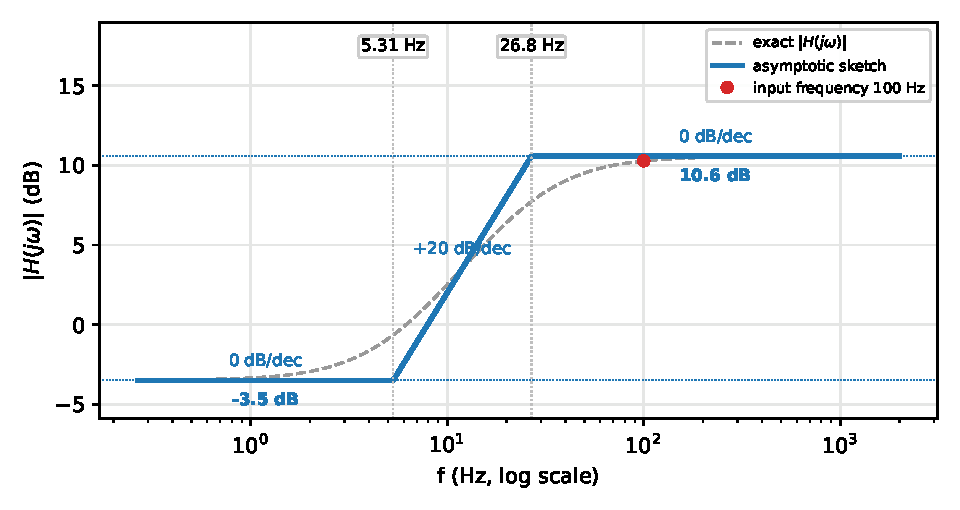
\includegraphics[width=0.78\linewidth,height=6.5cm,keepaspectratio]{p09_bode}\end{center}

{\small Blue: the straight-line sketch you are expected to draw. Dashed grey: the exact curve (about 3\,dB below the corner of an isolated pole). Red dot: the input frequency of Step 7.}
\solstep{7}{Steady-state output}The input is $V_i(t) = 0.01\sin\left(2\pi\cdot 100\,t\right)$, so $\omega_{in} = 2\pi\cdot 100 = 628$\,rad/s. Put $s=j\omega_{in}$ in each factor (tool T5): magnitudes multiply, angles add.
{\small Rules: $\left|\frac{s}{s+p}\right| = \frac{\omega}{\sqrt{\omega^2+p^2}}$, $\angle = \frac{\pi}{2}-\tan^{-1}\frac{\omega}{p}$;\quad $\left|\frac{1}{1+s/p}\right| = \frac{1}{\sqrt{1+(\omega/p)^2}}$, $\angle = -\tan^{-1}\frac{\omega}{p}$;\quad $\left|1+\frac{s}{z}\right| = \sqrt{1+(\omega/z)^2}$, $\angle = \tan^{-1}\frac{\omega}{z}$;\quad a negative $K$ adds $-\pi$.}
\begin{center}\renewcommand{\arraystretch}{1.35}
\begin{tabular}{ccc}
\toprule
factor & magnitude & angle (rad) \\
\midrule
$-0.668$ & $0.6684$ & $-3.14$ \\
$\rule[-1.1em]{0pt}{2.8em}\left(1+\dfrac{s}{2\pi\cdot 5.31}\right)$ & $18.88$ & $1.52$ \\
$\rule[-1.7em]{0pt}{4em}\dfrac{1}{1+\dfrac{s}{2\pi\cdot 26.8}}$ & $0.259$ & $-1.31$ \\
\textbf{total} & $\mathbf{3.267}$ (product) & $\mathbf{-2.93}$ (sum) \\
\bottomrule
\end{tabular}\end{center}

\begin{align*}
|H(j\omega_{in})| &= 3.27, \qquad \angle H(j\omega_{in}) = -2.93\ \mathrm{rad} \\
v_{o,ac}(t) &= 3.27\times 0.01\,\sin\left(2\pi\cdot 100\,t - 2.93\right) = 0.0327\,\sin\left(2\pi\cdot 100\,t - 2.93\right)
\end{align*}

\[
\boxed{V_o(t) = 0.0327\,\sin\left(2\pi\cdot 100\,t - 2.93\right)\ \mathrm{V}}
\]

\begin{ansbox}
$H(s) = -0.668\,\left(1+\dfrac{s}{2\pi\cdot 5.31}\right)\,\dfrac{1}{1+\dfrac{s}{2\pi\cdot 26.8}}$\quad (corners: 5.31 Hz, 26.8 Hz)\\[4pt]
$V_o(t) = 0.0327\,\sin\left(2\pi\cdot 100\,t - 2.93\right)\ \mathrm{V}$
\end{ansbox}

\newpage
\subsection*{Solution 5D.10 \hfill Medium}
\begin{center}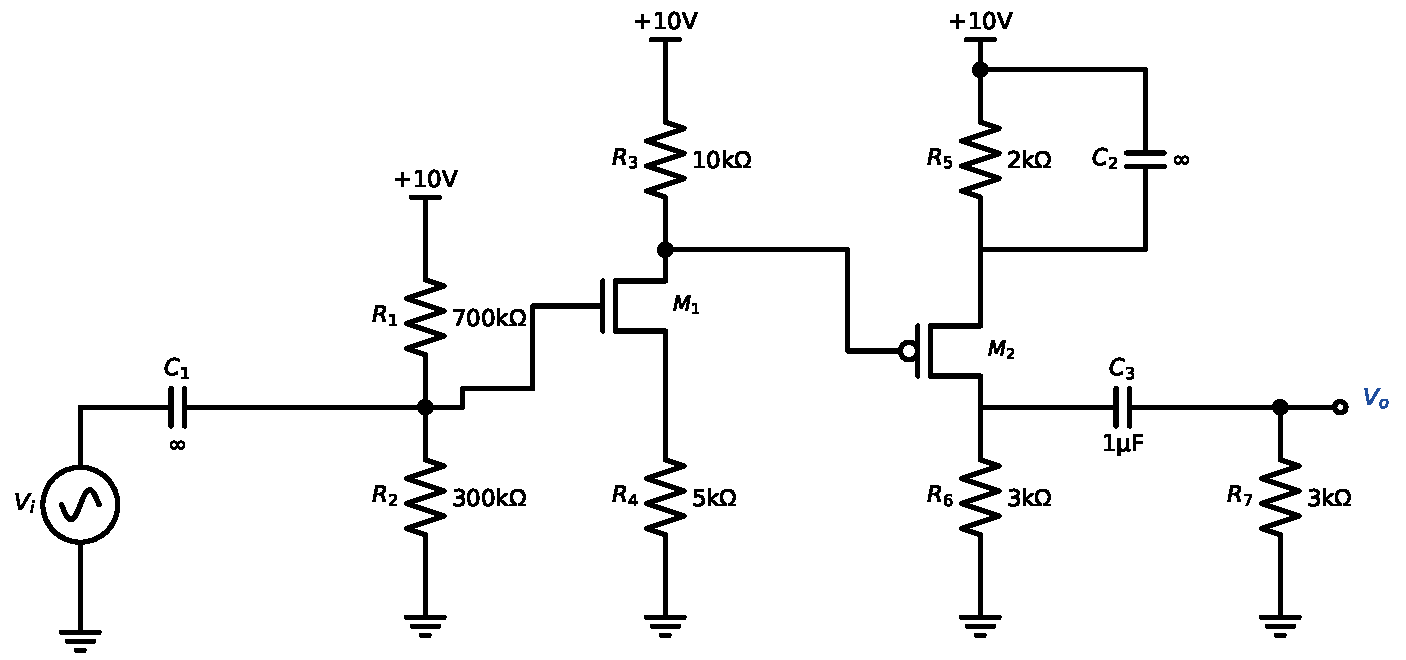
\includegraphics[width=0.9\linewidth,height=6cm,keepaspectratio]{p10_circuit}\end{center}
\solstep{1}{DC currents and transconductances}The DC drain currents are given: $I_{D1} = 200\,\mu \mathrm{A}$, $I_{D2} = 102\,\mu \mathrm{A}$. For AC every DC supply is ground and every ``$\infty$'' capacitor is a short. Transconductances (tool T4):\begin{align*}
g_{m1} &= k_{1}V_{ov1} = \sqrt{2k_{1}I_{D1}} = \sqrt{2\cdot1.1\,\mathrm{m}\mathrm{A/V^2}\cdot200\,\mu \mathrm{A}} = 663\,\mu \mathrm{A/V},\qquad \frac{1}{g_{m1}} = 1.51\,\mathrm{k}\Omega\quad(V_{ov1} = 0.602\,\mathrm{V}) \\
g_{m2} &= k_{2}V_{ov2} = \sqrt{2k_{2}I_{D2}} = \sqrt{2\cdot850\,\mu \mathrm{A/V^2}\cdot102\,\mu \mathrm{A}} = 417\,\mu \mathrm{A/V},\qquad \frac{1}{g_{m2}} = 2.4\,\mathrm{k}\Omega\quad(V_{ov2} = 0.491\,\mathrm{V})
\end{align*}

\solstep{2}{Input resistance of each stage}Input resistance of every stage, from the last back to the first (each one loads the stage before it):\begin{align*}
R_{i1} &= Z_{gate,1} = \infty\quad\text{(input at the gate: it loads nothing)} \\
R_{i2} &= Z_{gate,2} = \infty\quad\text{(input at the gate: it loads nothing)}
\end{align*}

\solstep{3}{Gain along the signal path}Multiply the node-to-node gains along the signal path (tool T4):\[
H(s) = \frac{v_{d1}}{v_{g1}}\cdot\frac{v_{d2}}{v_{g2}}\cdot\frac{v_o}{v_{d2}}
\]
\begin{align*}
\frac{v_{d1}}{v_{g1}} &= -\frac{Z_{D1}}{1/g_{m1} + Z_{S1}},\quad Z_{D1} = R_{3},\ Z_{S1} = R_{4}\ \Rightarrow\ -1.54 \\
\frac{v_{d2}}{v_{g2}} &= -\frac{Z_{D2}}{1/g_{m2} + Z_{S2}},\quad Z_{D2} = R_{6} \parallel \left(\frac{1}{sC_{3}} + R_{7}\right),\ Z_{S2} = 0\ \Rightarrow\ \dfrac{-0.626\,s - 209}{s + 167} \\
\frac{v_o}{v_{d2}} &= \frac{R_{7}}{\frac{1}{sC_{3}} + R_{7}} = \dfrac{s}{s + 333}
\end{align*}

\solstep{4}{Transfer function}Multiply and simplify:\[
H(s) = \dfrac{0.961\,s}{s + 167}
\]

\solstep{5}{Standard (Bode-ready) form}Find the roots. Every root $s=-p$ of the denominator is a \emph{pole}, every root $s=-z$ of the numerator is a \emph{zero}; $|p|$ and $|z|$ are the corner frequencies (rad/s).
\begin{itemize}[leftmargin=*,itemsep=2pt]
\item Numerator: it has the factor $s$ $\Rightarrow$ 1 zero at $s=0$.
\item Denominator: $s + 167$; $s + 167 = 0 \Rightarrow s = -167$.
\end{itemize}

Factored form (leading coefficient in front):
\[
H(s) = 0.961\,\dfrac{s}{(s+167)}
\]

Bode-ready form: rewrite every $(s+p) = p\left(1+\frac{s}{p}\right)$ and $(s+z) = z\left(1+\frac{s}{z}\right)$, and collect all constants into $K$. Each $s$ in the numerator is paired with one of the \emph{lowest} poles as $\frac{s}{s+p}$ (that factor is $\approx 1$ above $p$). Then every factor except $K$ is $\approx 1$ inside the pass-band:
\[
H(s) = 0.961\,\dfrac{s}{s+2\pi\cdot 26.5},\qquad K = 0.961
\]

\begin{center}\renewcommand{\arraystretch}{1.35}
\begin{tabular}{cccc}
\toprule
type & $\omega_c$ (rad/s) & $f_c=\omega_c/2\pi$ & slope change \\
\midrule
pole & $167$ & 26.5 Hz & $-20$ dB/dec \\
\bottomrule
\end{tabular}\end{center}

\solstep{6}{Magnitude Bode plot}Below every corner $|H(s)|\approx 0.00577\,s$, so the plot starts with a slope of $+20$\,dB/dec. Then, moving right, each pole bends the line down by 20\,dB/dec and each zero bends it up by 20\,dB/dec (tool T6):
\begin{center}\renewcommand{\arraystretch}{1.35}
\begin{tabular}{lcl}
\toprule
frequency range & slope & asymptote level \\
\midrule
$f<$ 26.5 Hz & $+20$ dB/dec & -0.344 dB at end \\
$f>$ 26.5 Hz & $0$ dB/dec (flat) & -0.344 dB at start \\
\bottomrule
\end{tabular}\end{center}

The flat (pass-band) level is $20\log_{10}|K| = 20\log_{10}0.961 = -0.344$\,dB.
\begin{center}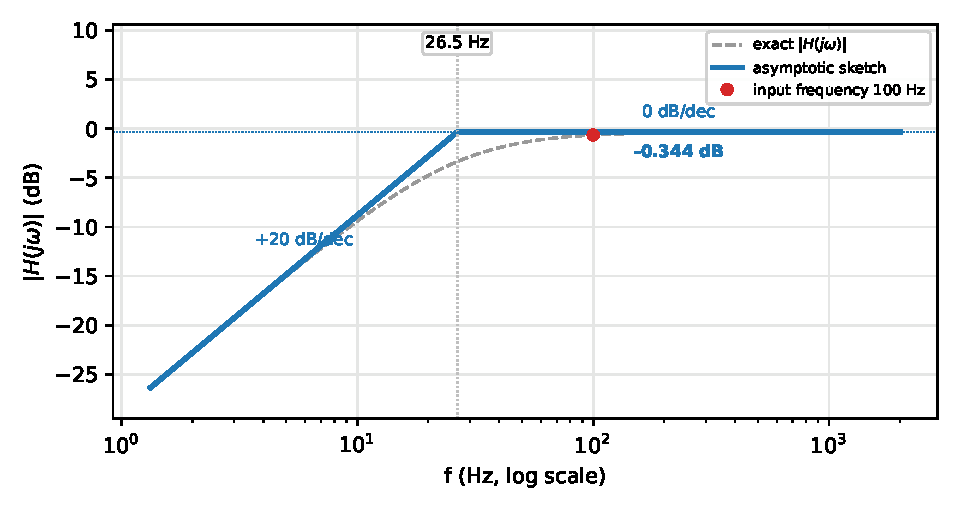
\includegraphics[width=0.78\linewidth,height=6.5cm,keepaspectratio]{p10_bode}\end{center}

{\small Blue: the straight-line sketch you are expected to draw. Dashed grey: the exact curve (about 3\,dB below the corner of an isolated pole). Red dot: the input frequency of Step 7.}
\solstep{7}{Steady-state output}The input is $V_i(t) = 0.002\sin\left(2\pi\cdot 100\,t\right)$, so $\omega_{in} = 2\pi\cdot 100 = 628$\,rad/s. Put $s=j\omega_{in}$ in each factor (tool T5): magnitudes multiply, angles add.
{\small Rules: $\left|\frac{s}{s+p}\right| = \frac{\omega}{\sqrt{\omega^2+p^2}}$, $\angle = \frac{\pi}{2}-\tan^{-1}\frac{\omega}{p}$;\quad $\left|\frac{1}{1+s/p}\right| = \frac{1}{\sqrt{1+(\omega/p)^2}}$, $\angle = -\tan^{-1}\frac{\omega}{p}$;\quad $\left|1+\frac{s}{z}\right| = \sqrt{1+(\omega/z)^2}$, $\angle = \tan^{-1}\frac{\omega}{z}$;\quad a negative $K$ adds $-\pi$.}
\begin{center}\renewcommand{\arraystretch}{1.35}
\begin{tabular}{ccc}
\toprule
factor & magnitude & angle (rad) \\
\midrule
$0.961$ & $0.9611$ & $0$ \\
$\rule[-1.1em]{0pt}{2.8em}\dfrac{s}{s+2\pi\cdot 26.5}$ & $0.9666$ & $0.259$ \\
\textbf{total} & $\mathbf{0.929}$ (product) & $\mathbf{0.259}$ (sum) \\
\bottomrule
\end{tabular}\end{center}

\begin{align*}
|H(j\omega_{in})| &= 0.929, \qquad \angle H(j\omega_{in}) = 0.259\ \mathrm{rad} \\
v_{o,ac}(t) &= 0.929\times 0.002\,\sin\left(2\pi\cdot 100\,t + 0.259\right) = 0.00186\,\sin\left(2\pi\cdot 100\,t + 0.259\right)
\end{align*}

\[
\boxed{V_o(t) = 0.00186\,\sin\left(2\pi\cdot 100\,t + 0.259\right)\ \mathrm{V}}
\]

\begin{ansbox}
$H(s) = 0.961\,\dfrac{s}{s+2\pi\cdot 26.5}$\quad (corners: 26.5 Hz)\\[4pt]
$V_o(t) = 0.00186\,\sin\left(2\pi\cdot 100\,t + 0.259\right)\ \mathrm{V}$
\end{ansbox}

\newpage
\subsection*{Solution 5D.11 \hfill Medium}
\begin{center}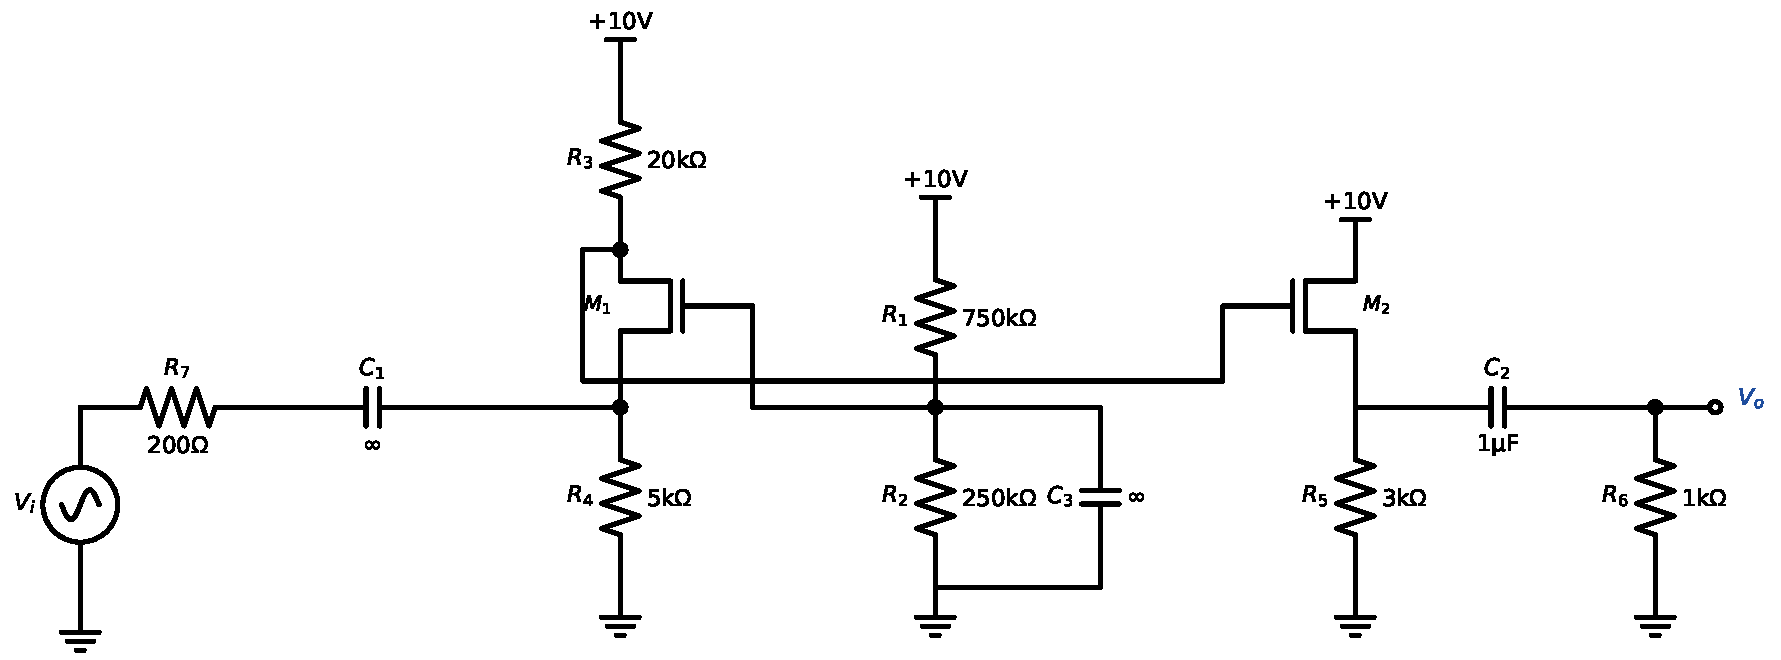
\includegraphics[width=0.9\linewidth,height=6cm,keepaspectratio]{p11_circuit}\end{center}
\solstep{1}{DC currents and transconductances}The DC drain currents are given: $I_{D1} = 209\,\mu \mathrm{A}$, $I_{D2} = 1.24\,\mathrm{m}\mathrm{A}$. For AC every DC supply is ground and every ``$\infty$'' capacitor is a short. Transconductances (tool T4):\begin{align*}
g_{m1} &= k_{1}V_{ov1} = \sqrt{2k_{1}I_{D1}} = \sqrt{2\cdot2\,\mathrm{m}\mathrm{A/V^2}\cdot209\,\mu \mathrm{A}} = 914\,\mu \mathrm{A/V},\qquad \frac{1}{g_{m1}} = 1.09\,\mathrm{k}\Omega\quad(V_{ov1} = 0.457\,\mathrm{V}) \\
g_{m2} &= k_{2}V_{ov2} = \sqrt{2k_{2}I_{D2}} = \sqrt{2\cdot2\,\mathrm{m}\mathrm{A/V^2}\cdot1.24\,\mathrm{m}\mathrm{A}} = 2.23\,\mathrm{m}\mathrm{A/V},\qquad \frac{1}{g_{m2}} = 449\,\Omega\quad(V_{ov2} = 1.11\,\mathrm{V})
\end{align*}

\solstep{2}{Input resistance of each stage}Input resistance of every stage, from the last back to the first (each one loads the stage before it):\begin{align*}
R_{i1} &= Z_{source,1} = \frac{1}{g_{m1}} = 1.09\,\mathrm{k}\Omega\quad\text{(common gate)} \\
R_{i2} &= Z_{gate,2} = \infty\quad\text{(input at the gate: it loads nothing)}
\end{align*}

\solstep{3}{Gain along the signal path}Multiply the node-to-node gains along the signal path (tool T4):\[
H(s) = \frac{v_{s1}}{v_i}\cdot\frac{v_{d1}}{v_{s1}}\cdot\frac{v_{s2}}{v_{g2}}\cdot\frac{v_o}{v_{s2}}
\]
\begin{align*}
\frac{v_{s1}}{v_i} &= \frac{R_{4} \parallel R_{i1}}{R_{7} + R_{4} \parallel R_{i1}} = 0.818 \\
\frac{v_{d1}}{v_{s1}} &= \frac{Z_{D1}}{1/g_{m1}},\quad Z_{D1} = R_{3}\ \Rightarrow\ 18.3 \\
\frac{v_{s2}}{v_{g2}} &= \frac{Z_{S2}}{1/g_{m2} + Z_{S2}},\quad Z_{S2} = R_{5} \parallel \left(\frac{1}{sC_{2}} + R_{6}\right)\ \Rightarrow\ \dfrac{0.625\,s + 625}{s + 719} \\
\frac{v_o}{v_{s2}} &= \frac{R_{6}}{\frac{1}{sC_{2}} + R_{6}} = \dfrac{s}{s + 1000}
\end{align*}

\solstep{4}{Transfer function}Multiply and simplify:\[
H(s) = \dfrac{9.34\,s}{s + 719}
\]

\solstep{5}{Standard (Bode-ready) form}Find the roots. Every root $s=-p$ of the denominator is a \emph{pole}, every root $s=-z$ of the numerator is a \emph{zero}; $|p|$ and $|z|$ are the corner frequencies (rad/s).
\begin{itemize}[leftmargin=*,itemsep=2pt]
\item Numerator: it has the factor $s$ $\Rightarrow$ 1 zero at $s=0$.
\item Denominator: $s + 719$; $s + 719 = 0 \Rightarrow s = -719$.
\end{itemize}

Factored form (leading coefficient in front):
\[
H(s) = 9.34\,\dfrac{s}{(s+719)}
\]

Bode-ready form: rewrite every $(s+p) = p\left(1+\frac{s}{p}\right)$ and $(s+z) = z\left(1+\frac{s}{z}\right)$, and collect all constants into $K$. Each $s$ in the numerator is paired with one of the \emph{lowest} poles as $\frac{s}{s+p}$ (that factor is $\approx 1$ above $p$). Then every factor except $K$ is $\approx 1$ inside the pass-band:
\[
H(s) = 9.34\,\dfrac{s}{s+2\pi\cdot 114},\qquad K = 9.34
\]

\begin{center}\renewcommand{\arraystretch}{1.35}
\begin{tabular}{cccc}
\toprule
type & $\omega_c$ (rad/s) & $f_c=\omega_c/2\pi$ & slope change \\
\midrule
pole & $719$ & 114 Hz & $-20$ dB/dec \\
\bottomrule
\end{tabular}\end{center}

\solstep{6}{Magnitude Bode plot}Below every corner $|H(s)|\approx 0.013\,s$, so the plot starts with a slope of $+20$\,dB/dec. Then, moving right, each pole bends the line down by 20\,dB/dec and each zero bends it up by 20\,dB/dec (tool T6):
\begin{center}\renewcommand{\arraystretch}{1.35}
\begin{tabular}{lcl}
\toprule
frequency range & slope & asymptote level \\
\midrule
$f<$ 114 Hz & $+20$ dB/dec & 19.4 dB at end \\
$f>$ 114 Hz & $0$ dB/dec (flat) & 19.4 dB at start \\
\bottomrule
\end{tabular}\end{center}

The flat (pass-band) level is $20\log_{10}|K| = 20\log_{10}9.34 = 19.4$\,dB.
\begin{center}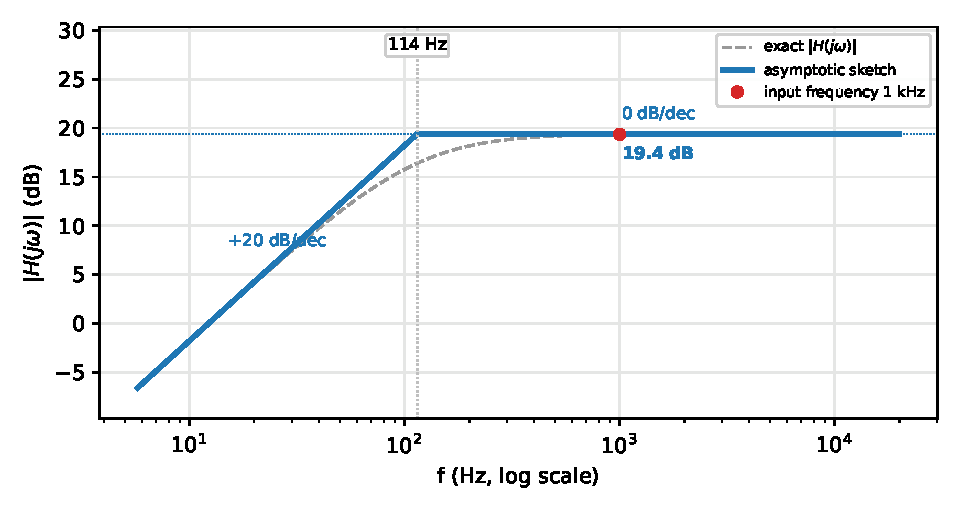
\includegraphics[width=0.78\linewidth,height=6.5cm,keepaspectratio]{p11_bode}\end{center}

{\small Blue: the straight-line sketch you are expected to draw. Dashed grey: the exact curve (about 3\,dB below the corner of an isolated pole). Red dot: the input frequency of Step 7.}
\solstep{7}{Steady-state output}The input is $V_i(t) = 0.005\sin\left(2\pi\cdot 1000\,t\right)$, so $\omega_{in} = 2\pi\cdot 1000 = 6280$\,rad/s. Put $s=j\omega_{in}$ in each factor (tool T5): magnitudes multiply, angles add.
{\small Rules: $\left|\frac{s}{s+p}\right| = \frac{\omega}{\sqrt{\omega^2+p^2}}$, $\angle = \frac{\pi}{2}-\tan^{-1}\frac{\omega}{p}$;\quad $\left|\frac{1}{1+s/p}\right| = \frac{1}{\sqrt{1+(\omega/p)^2}}$, $\angle = -\tan^{-1}\frac{\omega}{p}$;\quad $\left|1+\frac{s}{z}\right| = \sqrt{1+(\omega/z)^2}$, $\angle = \tan^{-1}\frac{\omega}{z}$;\quad a negative $K$ adds $-\pi$.}
\begin{center}\renewcommand{\arraystretch}{1.35}
\begin{tabular}{ccc}
\toprule
factor & magnitude & angle (rad) \\
\midrule
$9.34$ & $9.344$ & $0$ \\
$\rule[-1.1em]{0pt}{2.8em}\dfrac{s}{s+2\pi\cdot 114}$ & $0.9935$ & $0.114$ \\
\textbf{total} & $\mathbf{9.284}$ (product) & $\mathbf{0.114}$ (sum) \\
\bottomrule
\end{tabular}\end{center}

\begin{align*}
|H(j\omega_{in})| &= 9.28, \qquad \angle H(j\omega_{in}) = 0.114\ \mathrm{rad} \\
v_{o,ac}(t) &= 9.28\times 0.005\,\sin\left(2\pi\cdot 1000\,t + 0.114\right) = 0.0464\,\sin\left(2\pi\cdot 1000\,t + 0.114\right)
\end{align*}

\[
\boxed{V_o(t) = 0.0464\,\sin\left(2\pi\cdot 1000\,t + 0.114\right)\ \mathrm{V}}
\]

\begin{ansbox}
$H(s) = 9.34\,\dfrac{s}{s+2\pi\cdot 114}$\quad (corners: 114 Hz)\\[4pt]
$V_o(t) = 0.0464\,\sin\left(2\pi\cdot 1000\,t + 0.114\right)\ \mathrm{V}$
\end{ansbox}

\newpage
\subsection*{Solution 5D.12 \hfill Medium}
\begin{center}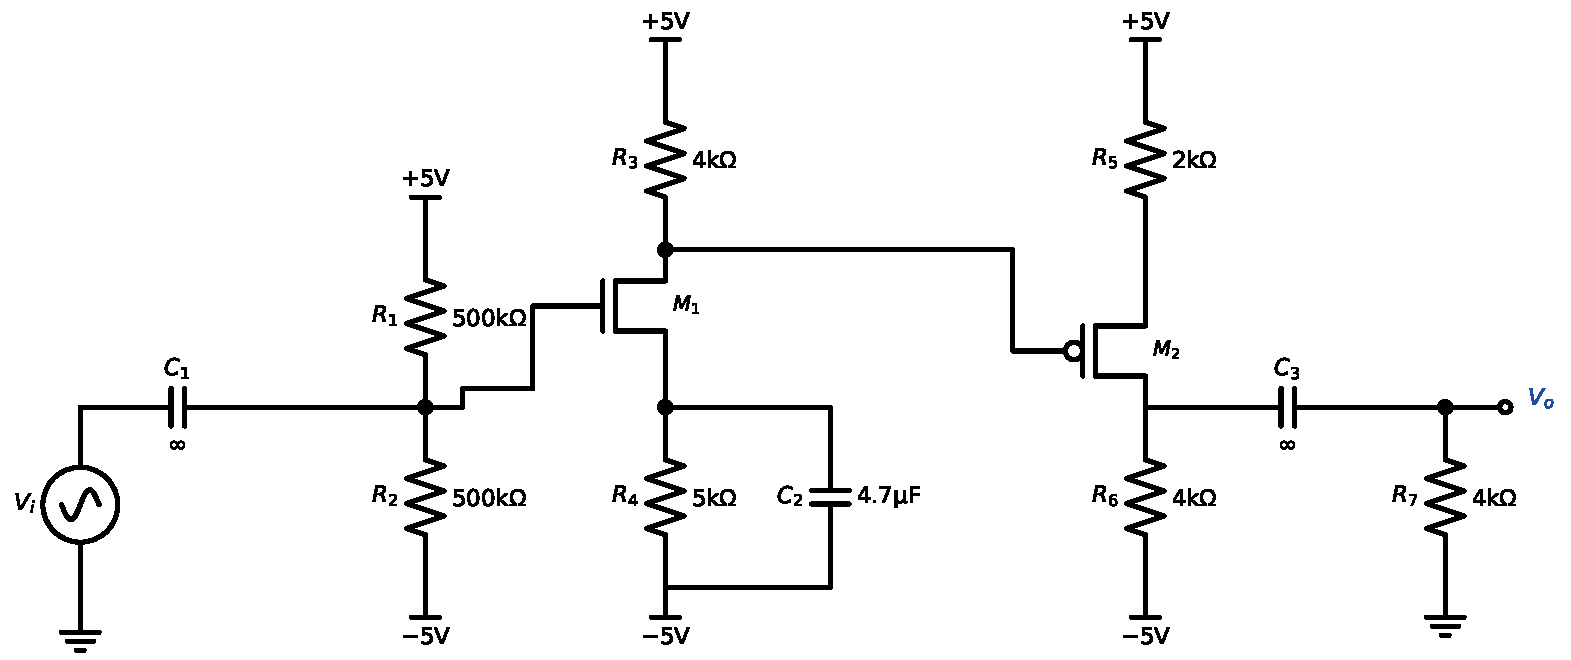
\includegraphics[width=0.9\linewidth,height=6cm,keepaspectratio]{p12_circuit}\end{center}
\solstep{1}{DC currents and transconductances}The DC drain currents are given: $I_{D1} = 640\,\mu \mathrm{A}$, $I_{D2} = 357\,\mu \mathrm{A}$. For AC every DC supply is ground and every ``$\infty$'' capacitor is a short. Transconductances (tool T4):\begin{align*}
g_{m1} &= k_{1}V_{ov1} = \sqrt{2k_{1}I_{D1}} = \sqrt{2\cdot2\,\mathrm{m}\mathrm{A/V^2}\cdot640\,\mu \mathrm{A}} = 1.6\,\mathrm{m}\mathrm{A/V},\qquad \frac{1}{g_{m1}} = 625\,\Omega\quad(V_{ov1} = 0.8\,\mathrm{V}) \\
g_{m2} &= k_{2}V_{ov2} = \sqrt{2k_{2}I_{D2}} = \sqrt{2\cdot1\,\mathrm{m}\mathrm{A/V^2}\cdot357\,\mu \mathrm{A}} = 845\,\mu \mathrm{A/V},\qquad \frac{1}{g_{m2}} = 1.18\,\mathrm{k}\Omega\quad(V_{ov2} = 0.845\,\mathrm{V})
\end{align*}

\solstep{2}{Input resistance of each stage}Input resistance of every stage, from the last back to the first (each one loads the stage before it):\begin{align*}
R_{i1} &= Z_{gate,1} = \infty\quad\text{(input at the gate: it loads nothing)} \\
R_{i2} &= Z_{gate,2} = \infty\quad\text{(input at the gate: it loads nothing)}
\end{align*}

\solstep{3}{Gain along the signal path}Multiply the node-to-node gains along the signal path (tool T4):\[
H(s) = \frac{v_{d1}}{v_{g1}}\cdot\frac{v_{d2}}{v_{g2}}
\]
\begin{align*}
\frac{v_{d1}}{v_{g1}} &= -\frac{Z_{D1}}{1/g_{m1} + Z_{S1}},\quad Z_{D1} = R_{3},\ Z_{S1} = R_{4} \parallel \frac{1}{sC_{2}}\ \Rightarrow\ \dfrac{-6.4\,s - 272}{s + 383} \\
\frac{v_{d2}}{v_{g2}} &= -\frac{Z_{D2}}{1/g_{m2} + Z_{S2}},\quad Z_{D2} = R_{6} \parallel R_{7},\ Z_{S2} = R_{5}\ \Rightarrow\ -0.628
\end{align*}

\solstep{4}{Transfer function}Multiply and simplify:\[
H(s) = \dfrac{4.02\,s + 171}{s + 383}
\]

\solstep{5}{Standard (Bode-ready) form}Find the roots. Every root $s=-p$ of the denominator is a \emph{pole}, every root $s=-z$ of the numerator is a \emph{zero}; $|p|$ and $|z|$ are the corner frequencies (rad/s).
\begin{itemize}[leftmargin=*,itemsep=2pt]
\item Numerator: $4.02\,s + 171$; divide by the leading coefficient $4.02$ (this does not move the roots): $s + 42.6$; $s + 42.6 = 0 \Rightarrow s = -42.6$.
\item Denominator: $s + 383$; $s + 383 = 0 \Rightarrow s = -383$.
\end{itemize}

Factored form (leading coefficient in front):
\[
H(s) = 4.02\,\dfrac{(s+42.6)}{(s+383)}
\]

Bode-ready form: rewrite every $(s+p) = p\left(1+\frac{s}{p}\right)$ and $(s+z) = z\left(1+\frac{s}{z}\right)$, and collect all constants into $K$. Then every factor except $K$ is $\approx 1$ inside the pass-band:
\[
H(s) = 0.447\,\left(1+\dfrac{s}{2\pi\cdot 6.77}\right)\,\dfrac{1}{1+\dfrac{s}{2\pi\cdot 61}},\qquad K = 0.447
\]

\begin{center}\renewcommand{\arraystretch}{1.35}
\begin{tabular}{cccc}
\toprule
type & $\omega_c$ (rad/s) & $f_c=\omega_c/2\pi$ & slope change \\
\midrule
zero & $42.6$ & 6.77 Hz & $+20$ dB/dec \\
pole & $383$ & 61 Hz & $-20$ dB/dec \\
\bottomrule
\end{tabular}\end{center}

\solstep{6}{Magnitude Bode plot}Below every corner, all factors are $\approx$ constant: $|H| \approx 0.447$ $= -7$\,dB (flat, 0 dB/dec). Then, moving right, each pole bends the line down by 20\,dB/dec and each zero bends it up by 20\,dB/dec (tool T6):
\begin{center}\renewcommand{\arraystretch}{1.35}
\begin{tabular}{lcl}
\toprule
frequency range & slope & asymptote level \\
\midrule
$f<$ 6.77 Hz & $0$ dB/dec (flat) & -7 dB at end \\
6.77 Hz -- 61 Hz & $+20$ dB/dec & -7 dB at start, 12.1 dB at end \\
$f>$ 61 Hz & $0$ dB/dec (flat) & 12.1 dB at start \\
\bottomrule
\end{tabular}\end{center}

\begin{center}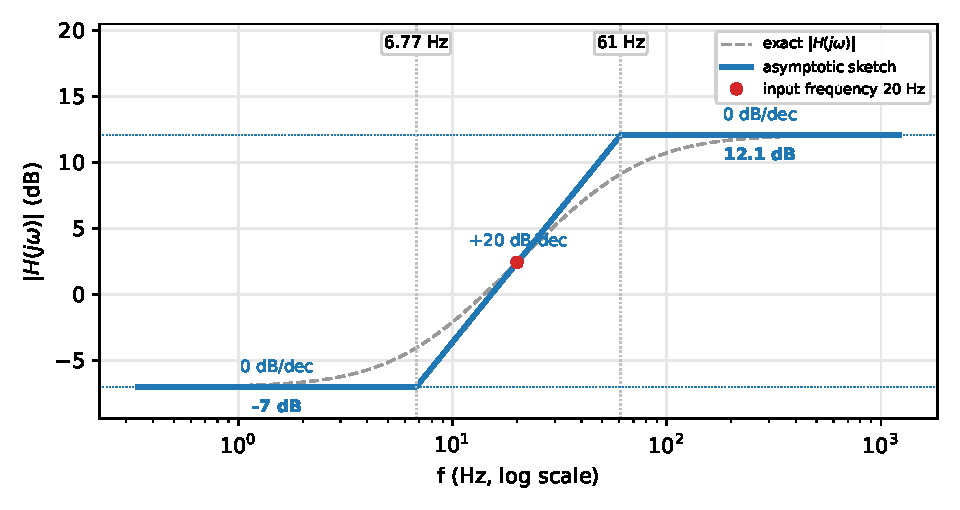
\includegraphics[width=0.78\linewidth,height=6.5cm,keepaspectratio]{p12_bode}\end{center}

{\small Blue: the straight-line sketch you are expected to draw. Dashed grey: the exact curve (about 3\,dB below the corner of an isolated pole). Red dot: the input frequency of Step 7.}
\solstep{7}{Steady-state output}The input is $V_i(t) = 0.005\sin\left(2\pi\cdot 20\,t\right)$, so $\omega_{in} = 2\pi\cdot 20 = 126$\,rad/s. Put $s=j\omega_{in}$ in each factor (tool T5): magnitudes multiply, angles add.
{\small Rules: $\left|\frac{s}{s+p}\right| = \frac{\omega}{\sqrt{\omega^2+p^2}}$, $\angle = \frac{\pi}{2}-\tan^{-1}\frac{\omega}{p}$;\quad $\left|\frac{1}{1+s/p}\right| = \frac{1}{\sqrt{1+(\omega/p)^2}}$, $\angle = -\tan^{-1}\frac{\omega}{p}$;\quad $\left|1+\frac{s}{z}\right| = \sqrt{1+(\omega/z)^2}$, $\angle = \tan^{-1}\frac{\omega}{z}$;\quad a negative $K$ adds $-\pi$.}
\begin{center}\renewcommand{\arraystretch}{1.35}
\begin{tabular}{ccc}
\toprule
factor & magnitude & angle (rad) \\
\midrule
$0.447$ & $0.4468$ & $0$ \\
$\rule[-1.1em]{0pt}{2.8em}\left(1+\dfrac{s}{2\pi\cdot 6.77}\right)$ & $3.118$ & $1.24$ \\
$\rule[-1.7em]{0pt}{4em}\dfrac{1}{1+\dfrac{s}{2\pi\cdot 61}}$ & $0.9502$ & $-0.317$ \\
\textbf{total} & $\mathbf{1.324}$ (product) & $\mathbf{0.927}$ (sum) \\
\bottomrule
\end{tabular}\end{center}

\begin{align*}
|H(j\omega_{in})| &= 1.32, \qquad \angle H(j\omega_{in}) = 0.927\ \mathrm{rad} \\
v_{o,ac}(t) &= 1.32\times 0.005\,\sin\left(2\pi\cdot 20\,t + 0.927\right) = 0.00662\,\sin\left(2\pi\cdot 20\,t + 0.927\right)
\end{align*}

\[
\boxed{V_o(t) = 0.00662\,\sin\left(2\pi\cdot 20\,t + 0.927\right)\ \mathrm{V}}
\]

\begin{ansbox}
$H(s) = 0.447\,\left(1+\dfrac{s}{2\pi\cdot 6.77}\right)\,\dfrac{1}{1+\dfrac{s}{2\pi\cdot 61}}$\quad (corners: 6.77 Hz, 61 Hz)\\[4pt]
$V_o(t) = 0.00662\,\sin\left(2\pi\cdot 20\,t + 0.927\right)\ \mathrm{V}$
\end{ansbox}

\newpage
\subsection*{Solution 5D.13 \hfill Hard}
\begin{center}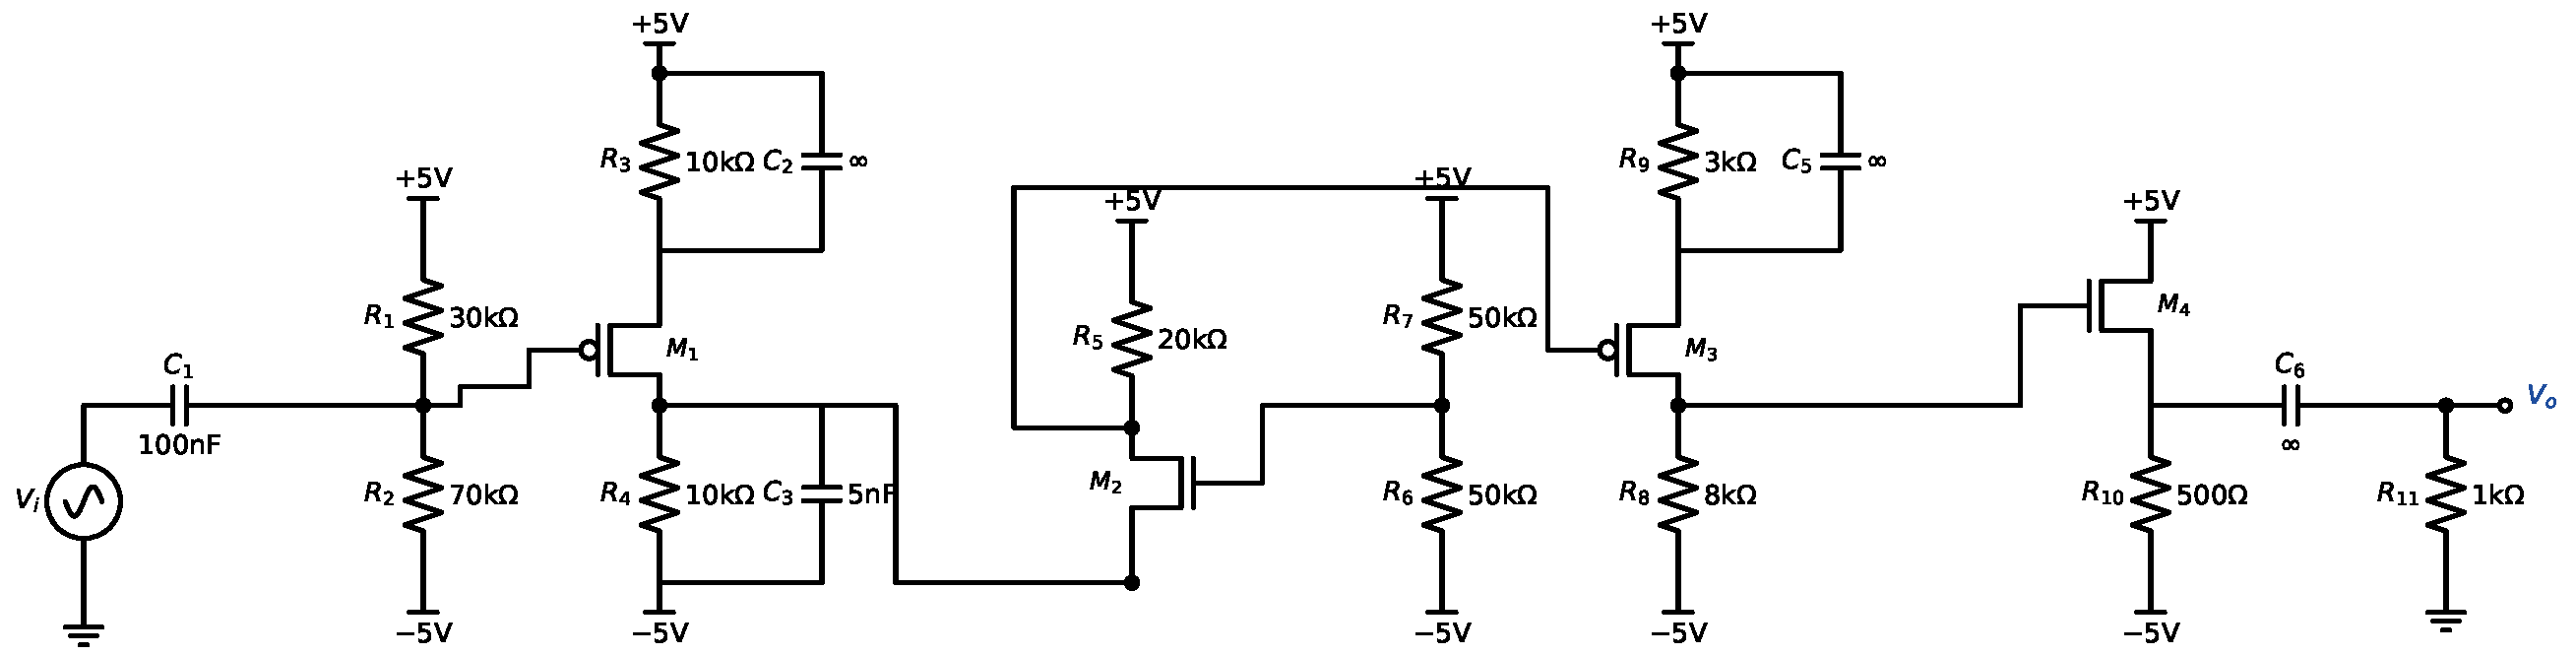
\includegraphics[width=0.9\linewidth,height=6cm,keepaspectratio]{p13_circuit}\end{center}
\solstep{1}{DC currents and transconductances}The DC drain currents are given: $I_{D1} = 117\,\mu \mathrm{A}$, $I_{D2} = 185\,\mu \mathrm{A}$, $I_{D3} = 453\,\mu \mathrm{A}$, $I_{D4} = 1.34\,\mathrm{m}\mathrm{A}$. For AC every DC supply is ground and every ``$\infty$'' capacitor is a short. Transconductances (tool T4):\begin{align*}
g_{m1} &= k_{1}V_{ov1} = \sqrt{2k_{1}I_{D1}} = \sqrt{2\cdot850\,\mu \mathrm{A/V^2}\cdot117\,\mu \mathrm{A}} = 447\,\mu \mathrm{A/V},\qquad \frac{1}{g_{m1}} = 2.24\,\mathrm{k}\Omega\quad(V_{ov1} = 0.526\,\mathrm{V}) \\
g_{m2} &= k_{2}V_{ov2} = \sqrt{2k_{2}I_{D2}} = \sqrt{2\cdot1.1\,\mathrm{m}\mathrm{A/V^2}\cdot185\,\mu \mathrm{A}} = 637\,\mu \mathrm{A/V},\qquad \frac{1}{g_{m2}} = 1.57\,\mathrm{k}\Omega\quad(V_{ov2} = 0.579\,\mathrm{V}) \\
g_{m3} &= k_{3}V_{ov3} = \sqrt{2k_{3}I_{D3}} = \sqrt{2\cdot850\,\mu \mathrm{A/V^2}\cdot453\,\mu \mathrm{A}} = 878\,\mu \mathrm{A/V},\qquad \frac{1}{g_{m3}} = 1.14\,\mathrm{k}\Omega\quad(V_{ov3} = 1.03\,\mathrm{V}) \\
g_{m4} &= k_{4}V_{ov4} = \sqrt{2k_{4}I_{D4}} = \sqrt{2\cdot1.1\,\mathrm{m}\mathrm{A/V^2}\cdot1.34\,\mathrm{m}\mathrm{A}} = 1.71\,\mathrm{m}\mathrm{A/V},\qquad \frac{1}{g_{m4}} = 583\,\Omega\quad(V_{ov4} = 1.56\,\mathrm{V})
\end{align*}

\solstep{2}{Input resistance of each stage}Input resistance of every stage, from the last back to the first (each one loads the stage before it):\begin{align*}
R_{i1} &= Z_{gate,1} = \infty\quad\text{(input at the gate: it loads nothing)} \\
R_{i2} &= Z_{source,2} = \frac{1}{g_{m2}} = 1.57\,\mathrm{k}\Omega\quad\text{(common gate)} \\
R_{i3} &= Z_{gate,3} = \infty\quad\text{(input at the gate: it loads nothing)} \\
R_{i4} &= Z_{gate,4} = \infty\quad\text{(input at the gate: it loads nothing)}
\end{align*}

\solstep{3}{Gain along the signal path}Multiply the node-to-node gains along the signal path (tool T4):\[
H(s) = \frac{v_{g1}}{v_i}\cdot\frac{v_{d1}}{v_{g1}}\cdot\frac{v_{d2}}{v_{s2}}\cdot\frac{v_{d3}}{v_{g3}}\cdot\frac{v_{s4}}{v_{g4}}
\]
\begin{align*}
\frac{v_{g1}}{v_i} &= \frac{R_{1} \parallel R_{2}}{\frac{1}{sC_{1}} + R_{1} \parallel R_{2}} = \dfrac{s}{s + 476} \\
\frac{v_{d1}}{v_{g1}} &= -\frac{Z_{D1}}{1/g_{m1} + Z_{S1}},\quad Z_{D1} = R_{4} \parallel \frac{1}{sC_{3}} \parallel R_{i2},\ Z_{S1} = 0\ \Rightarrow\ \dfrac{-89400}{s + 1.47\times 10^{5}} \\
\frac{v_{d2}}{v_{s2}} &= \frac{Z_{D2}}{1/g_{m2}},\quad Z_{D2} = R_{5}\ \Rightarrow\ 12.7 \\
\frac{v_{d3}}{v_{g3}} &= -\frac{Z_{D3}}{1/g_{m3} + Z_{S3}},\quad Z_{D3} = R_{8},\ Z_{S3} = 0\ \Rightarrow\ -7.02 \\
\frac{v_{s4}}{v_{g4}} &= \frac{Z_{S4}}{1/g_{m4} + Z_{S4}},\quad Z_{S4} = R_{10} \parallel R_{11}\ \Rightarrow\ 0.364
\end{align*}

\solstep{4}{Transfer function}Multiply and simplify:\[
H(s) = \dfrac{2.91\times 10^{6}\,s}{s^{2} + 1.48\times 10^{5}\,s + 7.02\times 10^{7}}
\]

\solstep{5}{Standard (Bode-ready) form}Find the roots. Every root $s=-p$ of the denominator is a \emph{pole}, every root $s=-z$ of the numerator is a \emph{zero}; $|p|$ and $|z|$ are the corner frequencies (rad/s).
\begin{itemize}[leftmargin=*,itemsep=2pt]
\item Numerator: it has the factor $s$ $\Rightarrow$ 1 zero at $s=0$.
\item Denominator: $s^{2} + 1.48\times 10^{5}\,s + 7.02\times 10^{7}$; quadratic formula:\[
s = \frac{-1.48\times 10^{5} \pm \sqrt{(1.48\times 10^{5})^2 - 4(7.02\times 10^{7})}}{2} = \frac{-1.48\times 10^{5} \pm 1.47\times 10^{5}}{2} \Rightarrow s = -476,\ -1.47\times 10^{5}
\]

\end{itemize}

Factored form (leading coefficient in front):
\[
H(s) = 2.91\times 10^{6}\,\dfrac{s}{(s+476)(s+1.47\times 10^{5})}
\]

Bode-ready form: rewrite every $(s+p) = p\left(1+\frac{s}{p}\right)$ and $(s+z) = z\left(1+\frac{s}{z}\right)$, and collect all constants into $K$. Each $s$ in the numerator is paired with one of the \emph{lowest} poles as $\frac{s}{s+p}$ (that factor is $\approx 1$ above $p$). Then every factor except $K$ is $\approx 1$ inside the pass-band:
\[
H(s) = 19.7\,\dfrac{s}{s+2\pi\cdot 75.8}\,\dfrac{1}{1+\dfrac{s}{2\pi\cdot 23.5\mathrm{k}}},\qquad K = 19.7
\]

\begin{center}\renewcommand{\arraystretch}{1.35}
\begin{tabular}{cccc}
\toprule
type & $\omega_c$ (rad/s) & $f_c=\omega_c/2\pi$ & slope change \\
\midrule
pole & $476$ & 75.8 Hz & $-20$ dB/dec \\
pole & $1.47\times 10^{5}$ & 23.5 kHz & $-20$ dB/dec \\
\bottomrule
\end{tabular}\end{center}

\solstep{6}{Magnitude Bode plot}Below every corner $|H(s)|\approx 0.0414\,s$, so the plot starts with a slope of $+20$\,dB/dec. Then, moving right, each pole bends the line down by 20\,dB/dec and each zero bends it up by 20\,dB/dec (tool T6):
\begin{center}\renewcommand{\arraystretch}{1.35}
\begin{tabular}{lcl}
\toprule
frequency range & slope & asymptote level \\
\midrule
$f<$ 75.8 Hz & $+20$ dB/dec & 25.9 dB at end \\
75.8 Hz -- 23.5 kHz & $0$ dB/dec (flat) & 25.9 dB at start, 25.9 dB at end \\
$f>$ 23.5 kHz & $-20$ dB/dec & 25.9 dB at start \\
\bottomrule
\end{tabular}\end{center}

The flat (pass-band) level is $20\log_{10}|K| = 20\log_{10}19.7 = 25.9$\,dB.
\begin{center}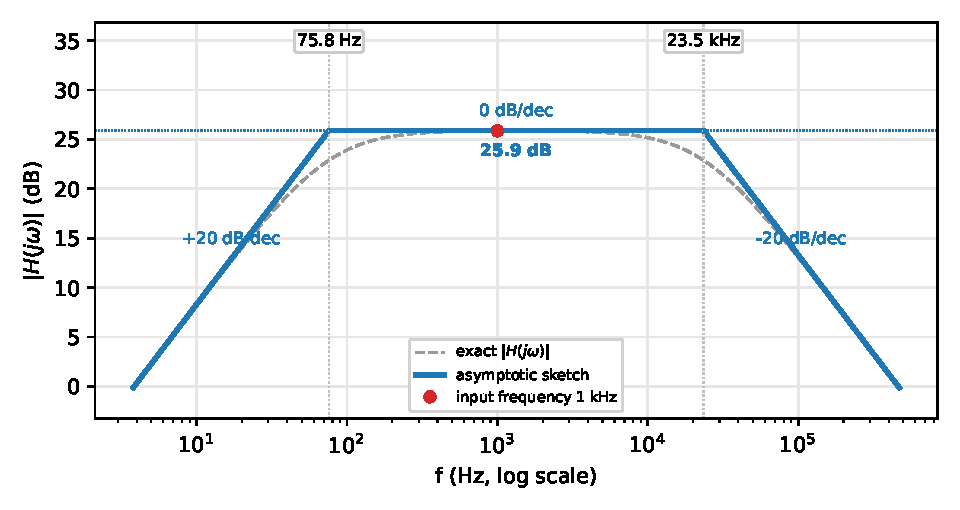
\includegraphics[width=0.78\linewidth,height=6.5cm,keepaspectratio]{p13_bode}\end{center}

{\small Blue: the straight-line sketch you are expected to draw. Dashed grey: the exact curve (about 3\,dB below the corner of an isolated pole). Red dot: the input frequency of Step 7.}
\solstep{7}{Steady-state output}The input is $V_i(t) = 0.005\sin\left(2\pi\cdot 1000\,t\right)$, so $\omega_{in} = 2\pi\cdot 1000 = 6280$\,rad/s. Put $s=j\omega_{in}$ in each factor (tool T5): magnitudes multiply, angles add.
{\small Rules: $\left|\frac{s}{s+p}\right| = \frac{\omega}{\sqrt{\omega^2+p^2}}$, $\angle = \frac{\pi}{2}-\tan^{-1}\frac{\omega}{p}$;\quad $\left|\frac{1}{1+s/p}\right| = \frac{1}{\sqrt{1+(\omega/p)^2}}$, $\angle = -\tan^{-1}\frac{\omega}{p}$;\quad $\left|1+\frac{s}{z}\right| = \sqrt{1+(\omega/z)^2}$, $\angle = \tan^{-1}\frac{\omega}{z}$;\quad a negative $K$ adds $-\pi$.}
\begin{center}\renewcommand{\arraystretch}{1.35}
\begin{tabular}{ccc}
\toprule
factor & magnitude & angle (rad) \\
\midrule
$19.7$ & $19.72$ & $0$ \\
$\rule[-1.1em]{0pt}{2.8em}\dfrac{s}{s+2\pi\cdot 75.8}$ & $0.9971$ & $0.0756$ \\
$\rule[-1.7em]{0pt}{4em}\dfrac{1}{1+\dfrac{s}{2\pi\cdot 23.5\mathrm{k}}}$ & $0.9991$ & $-0.0426$ \\
\textbf{total} & $\mathbf{19.65}$ (product) & $\mathbf{0.0331}$ (sum) \\
\bottomrule
\end{tabular}\end{center}

\begin{align*}
|H(j\omega_{in})| &= 19.7, \qquad \angle H(j\omega_{in}) = 0.0331\ \mathrm{rad} \\
v_{o,ac}(t) &= 19.7\times 0.005\,\sin\left(2\pi\cdot 1000\,t + 0.0331\right) = 0.0983\,\sin\left(2\pi\cdot 1000\,t + 0.0331\right)
\end{align*}

\[
\boxed{V_o(t) = 0.0983\,\sin\left(2\pi\cdot 1000\,t + 0.0331\right)\ \mathrm{V}}
\]

\begin{ansbox}
$H(s) = 19.7\,\dfrac{s}{s+2\pi\cdot 75.8}\,\dfrac{1}{1+\dfrac{s}{2\pi\cdot 23.5\mathrm{k}}}$\quad (corners: 75.8 Hz, 23.5 kHz)\\[4pt]
$V_o(t) = 0.0983\,\sin\left(2\pi\cdot 1000\,t + 0.0331\right)\ \mathrm{V}$
\end{ansbox}

\newpage
\subsection*{Solution 5D.14 \hfill Hard}
\begin{center}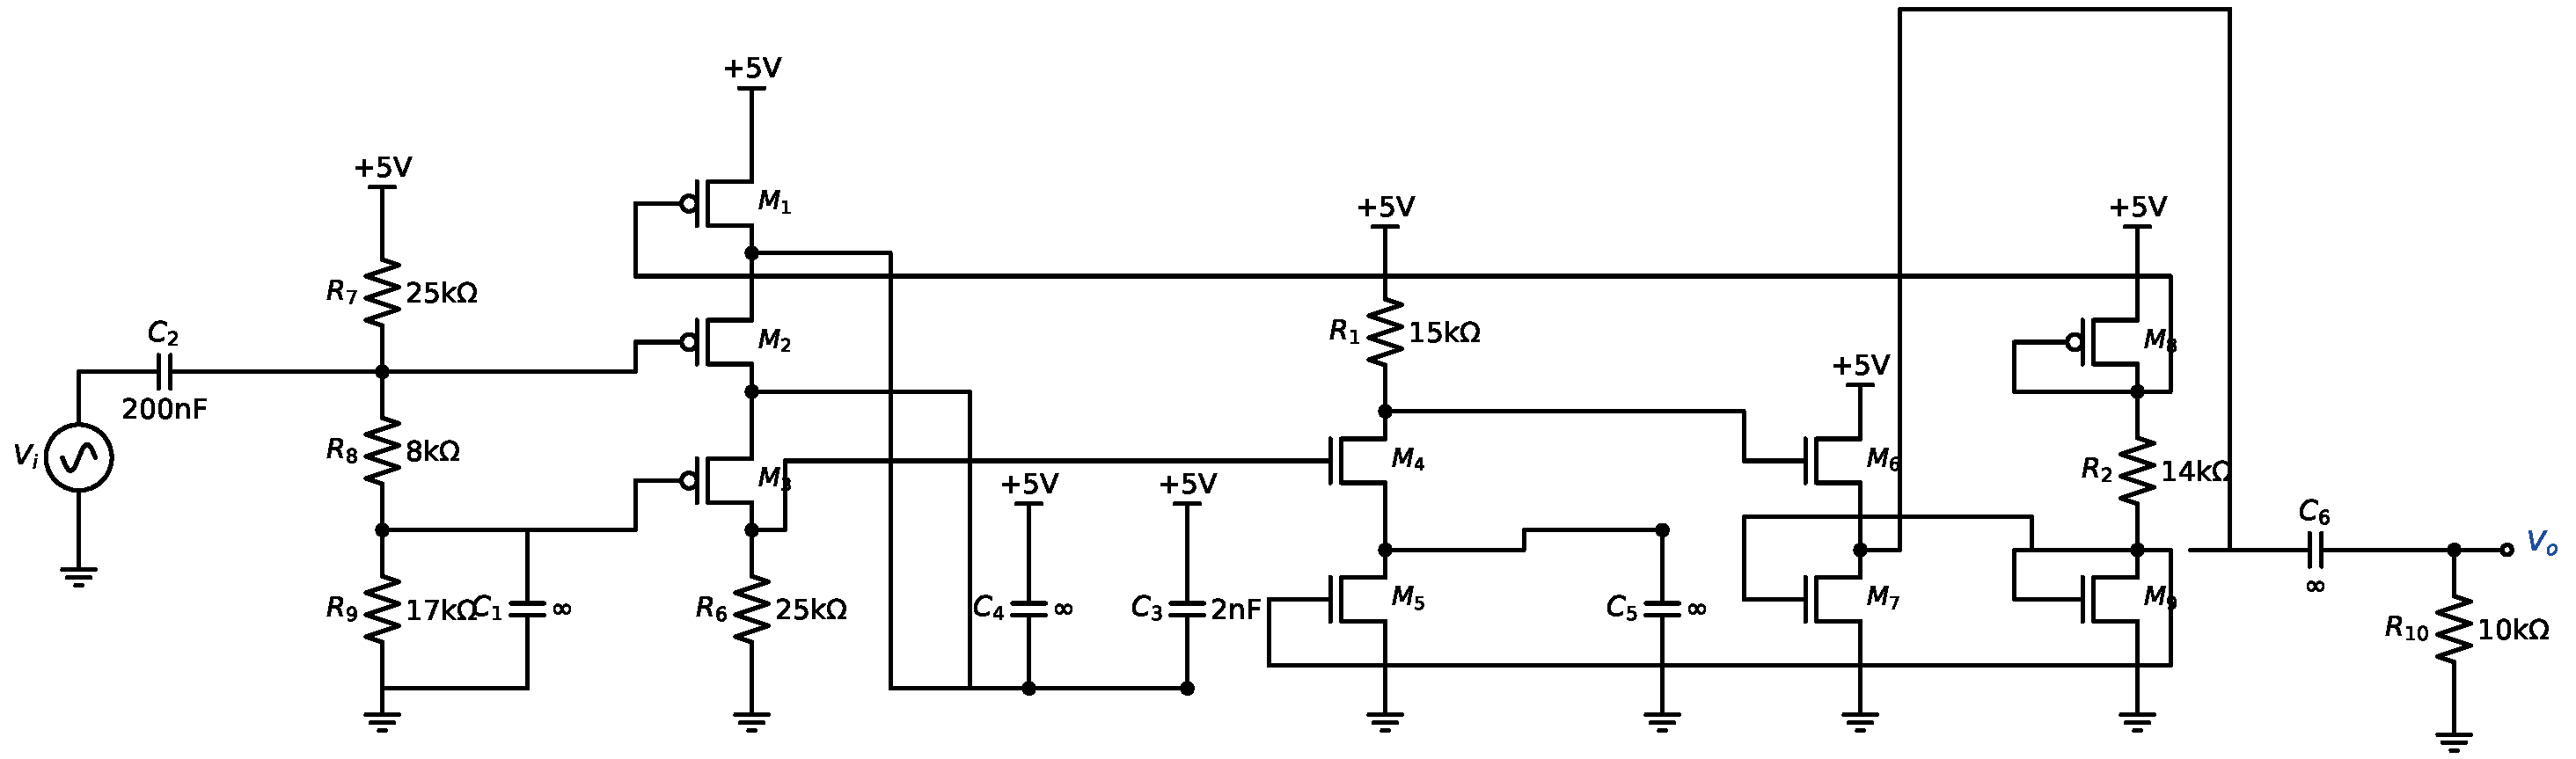
\includegraphics[width=0.9\linewidth,height=6cm,keepaspectratio]{p14_circuit}\end{center}
\solstep{1}{DC currents and transconductances}The DC drain currents are given: $I_{D2} = 99.4\,\mu \mathrm{A}$, $I_{D3} = 99.4\,\mu \mathrm{A}$, $I_{D4} = 99.4\,\mu \mathrm{A}$, $I_{D6} = 99.4\,\mu \mathrm{A}$. For AC every DC supply is ground and every ``$\infty$'' capacitor is a short. Transconductances (tool T4):\begin{align*}
g_{m2} &= k_{2}V_{ov2} = \sqrt{2k_{2}I_{D2}} = \sqrt{2\cdot850\,\mu \mathrm{A/V^2}\cdot99.4\,\mu \mathrm{A}} = 411\,\mu \mathrm{A/V},\qquad \frac{1}{g_{m2}} = 2.43\,\mathrm{k}\Omega\quad(V_{ov2} = 0.484\,\mathrm{V}) \\
g_{m3} &= k_{3}V_{ov3} = \sqrt{2k_{3}I_{D3}} = \sqrt{2\cdot850\,\mu \mathrm{A/V^2}\cdot99.4\,\mu \mathrm{A}} = 411\,\mu \mathrm{A/V},\qquad \frac{1}{g_{m3}} = 2.43\,\mathrm{k}\Omega\quad(V_{ov3} = 0.484\,\mathrm{V}) \\
g_{m4} &= k_{4}V_{ov4} = \sqrt{2k_{4}I_{D4}} = \sqrt{2\cdot1.1\,\mathrm{m}\mathrm{A/V^2}\cdot99.4\,\mu \mathrm{A}} = 468\,\mu \mathrm{A/V},\qquad \frac{1}{g_{m4}} = 2.14\,\mathrm{k}\Omega\quad(V_{ov4} = 0.425\,\mathrm{V}) \\
g_{m6} &= k_{6}V_{ov6} = \sqrt{2k_{6}I_{D6}} = \sqrt{2\cdot1.1\,\mathrm{m}\mathrm{A/V^2}\cdot99.4\,\mu \mathrm{A}} = 468\,\mu \mathrm{A/V},\qquad \frac{1}{g_{m6}} = 2.14\,\mathrm{k}\Omega\quad(V_{ov6} = 0.425\,\mathrm{V})
\end{align*}

\solstep{2}{Input resistance of each stage}Input resistance of every stage, from the last back to the first (each one loads the stage before it):\begin{align*}
R_{i2} &= Z_{gate,2} = \infty\quad\text{(input at the gate: it loads nothing)} \\
R_{i3} &= Z_{source,3} = \frac{1}{g_{m3}} = 2.43\,\mathrm{k}\Omega\quad\text{(common gate)} \\
R_{i4} &= Z_{gate,4} = \infty\quad\text{(input at the gate: it loads nothing)} \\
R_{i6} &= Z_{gate,6} = \infty\quad\text{(input at the gate: it loads nothing)}
\end{align*}

\solstep{3}{Gain along the signal path}Multiply the node-to-node gains along the signal path (tool T4):\[
H(s) = \frac{v_{g2}}{v_i}\cdot\frac{v_{d2}}{v_{g2}}\cdot\frac{v_{d3}}{v_{s3}}\cdot\frac{v_{d4}}{v_{g4}}\cdot\frac{v_{s6}}{v_{g6}}
\]
\begin{align*}
\frac{v_{g2}}{v_i} &= \frac{R_{7} \parallel R_{8}}{\frac{1}{sC_{2}} + R_{7} \parallel R_{8}} = \dfrac{s}{s + 825} \\
\frac{v_{d2}}{v_{g2}} &= -\frac{Z_{D2}}{1/g_{m2} + Z_{S2}},\quad Z_{D2} = \frac{1}{sC_{3}} \parallel R_{i3},\ Z_{S2} = 0\ \Rightarrow\ \dfrac{-2.06\times 10^{5}}{s + 2.06\times 10^{5}} \\
\frac{v_{d3}}{v_{s3}} &= \frac{Z_{D3}}{1/g_{m3}},\quad Z_{D3} = R_{6}\ \Rightarrow\ 10.3 \\
\frac{v_{d4}}{v_{g4}} &= -\frac{Z_{D4}}{1/g_{m4} + Z_{S4}},\quad Z_{D4} = R_{1},\ Z_{S4} = 0\ \Rightarrow\ -7.01 \\
\frac{v_{s6}}{v_{g6}} &= \frac{Z_{S6}}{1/g_{m6} + Z_{S6}},\quad Z_{S6} = R_{10}\ \Rightarrow\ 0.824
\end{align*}

\solstep{4}{Transfer function}Multiply and simplify:\[
H(s) = \dfrac{1.22\times 10^{7}\,s}{s^{2} + 2.06\times 10^{5}\,s + 1.7\times 10^{8}}
\]

\solstep{5}{Standard (Bode-ready) form}Find the roots. Every root $s=-p$ of the denominator is a \emph{pole}, every root $s=-z$ of the numerator is a \emph{zero}; $|p|$ and $|z|$ are the corner frequencies (rad/s).
\begin{itemize}[leftmargin=*,itemsep=2pt]
\item Numerator: it has the factor $s$ $\Rightarrow$ 1 zero at $s=0$.
\item Denominator: $s^{2} + 2.06\times 10^{5}\,s + 1.7\times 10^{8}$; quadratic formula:\[
s = \frac{-2.06\times 10^{5} \pm \sqrt{(2.06\times 10^{5})^2 - 4(1.7\times 10^{8})}}{2} = \frac{-2.06\times 10^{5} \pm 2.05\times 10^{5}}{2} \Rightarrow s = -825,\ -2.06\times 10^{5}
\]

\end{itemize}

Factored form (leading coefficient in front):
\[
H(s) = 1.22\times 10^{7}\,\dfrac{s}{(s+825)(s+2.06\times 10^{5})}
\]

Bode-ready form: rewrite every $(s+p) = p\left(1+\frac{s}{p}\right)$ and $(s+z) = z\left(1+\frac{s}{z}\right)$, and collect all constants into $K$. Each $s$ in the numerator is paired with one of the \emph{lowest} poles as $\frac{s}{s+p}$ (that factor is $\approx 1$ above $p$). Then every factor except $K$ is $\approx 1$ inside the pass-band:
\[
H(s) = 59.4\,\dfrac{s}{s+2\pi\cdot 131}\,\dfrac{1}{1+\dfrac{s}{2\pi\cdot 32.7\mathrm{k}}},\qquad K = 59.4
\]

\begin{center}\renewcommand{\arraystretch}{1.35}
\begin{tabular}{cccc}
\toprule
type & $\omega_c$ (rad/s) & $f_c=\omega_c/2\pi$ & slope change \\
\midrule
pole & $825$ & 131 Hz & $-20$ dB/dec \\
pole & $2.06\times 10^{5}$ & 32.7 kHz & $-20$ dB/dec \\
\bottomrule
\end{tabular}\end{center}

\solstep{6}{Magnitude Bode plot}Below every corner $|H(s)|\approx 0.072\,s$, so the plot starts with a slope of $+20$\,dB/dec. Then, moving right, each pole bends the line down by 20\,dB/dec and each zero bends it up by 20\,dB/dec (tool T6):
\begin{center}\renewcommand{\arraystretch}{1.35}
\begin{tabular}{lcl}
\toprule
frequency range & slope & asymptote level \\
\midrule
$f<$ 131 Hz & $+20$ dB/dec & 35.5 dB at end \\
131 Hz -- 32.7 kHz & $0$ dB/dec (flat) & 35.5 dB at start, 35.5 dB at end \\
$f>$ 32.7 kHz & $-20$ dB/dec & 35.5 dB at start \\
\bottomrule
\end{tabular}\end{center}

The flat (pass-band) level is $20\log_{10}|K| = 20\log_{10}59.4 = 35.5$\,dB.
\begin{center}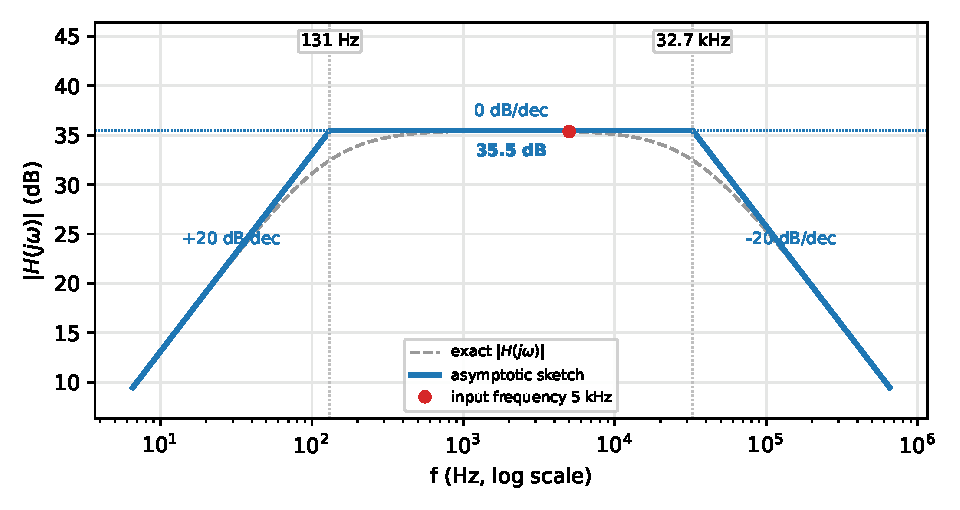
\includegraphics[width=0.78\linewidth,height=6.5cm,keepaspectratio]{p14_bode}\end{center}

{\small Blue: the straight-line sketch you are expected to draw. Dashed grey: the exact curve (about 3\,dB below the corner of an isolated pole). Red dot: the input frequency of Step 7.}
\solstep{7}{Steady-state output}The input is $V_i(t) = 0.01\sin\left(2\pi\cdot 5000\,t\right)$, so $\omega_{in} = 2\pi\cdot 5000 = 31400$\,rad/s. Put $s=j\omega_{in}$ in each factor (tool T5): magnitudes multiply, angles add.
{\small Rules: $\left|\frac{s}{s+p}\right| = \frac{\omega}{\sqrt{\omega^2+p^2}}$, $\angle = \frac{\pi}{2}-\tan^{-1}\frac{\omega}{p}$;\quad $\left|\frac{1}{1+s/p}\right| = \frac{1}{\sqrt{1+(\omega/p)^2}}$, $\angle = -\tan^{-1}\frac{\omega}{p}$;\quad $\left|1+\frac{s}{z}\right| = \sqrt{1+(\omega/z)^2}$, $\angle = \tan^{-1}\frac{\omega}{z}$;\quad a negative $K$ adds $-\pi$.}
\begin{center}\renewcommand{\arraystretch}{1.35}
\begin{tabular}{ccc}
\toprule
factor & magnitude & angle (rad) \\
\midrule
$59.4$ & $59.38$ & $0$ \\
$\rule[-1.1em]{0pt}{2.8em}\dfrac{s}{s+2\pi\cdot 131}$ & $0.9997$ & $0.0263$ \\
$\rule[-1.7em]{0pt}{4em}\dfrac{1}{1+\dfrac{s}{2\pi\cdot 32.7\mathrm{k}}}$ & $0.9885$ & $-0.152$ \\
\textbf{total} & $\mathbf{58.67}$ (product) & $\mathbf{-0.125}$ (sum) \\
\bottomrule
\end{tabular}\end{center}

\begin{align*}
|H(j\omega_{in})| &= 58.7, \qquad \angle H(j\omega_{in}) = -0.125\ \mathrm{rad} \\
v_{o,ac}(t) &= 58.7\times 0.01\,\sin\left(2\pi\cdot 5000\,t - 0.125\right) = 0.587\,\sin\left(2\pi\cdot 5000\,t - 0.125\right)
\end{align*}

\[
\boxed{V_o(t) = 0.587\,\sin\left(2\pi\cdot 5000\,t - 0.125\right)\ \mathrm{V}}
\]

\begin{ansbox}
$H(s) = 59.4\,\dfrac{s}{s+2\pi\cdot 131}\,\dfrac{1}{1+\dfrac{s}{2\pi\cdot 32.7\mathrm{k}}}$\quad (corners: 131 Hz, 32.7 kHz)\\[4pt]
$V_o(t) = 0.587\,\sin\left(2\pi\cdot 5000\,t - 0.125\right)\ \mathrm{V}$
\end{ansbox}

\newpage
\subsection*{Solution 5D.15 \hfill Hard}
\begin{center}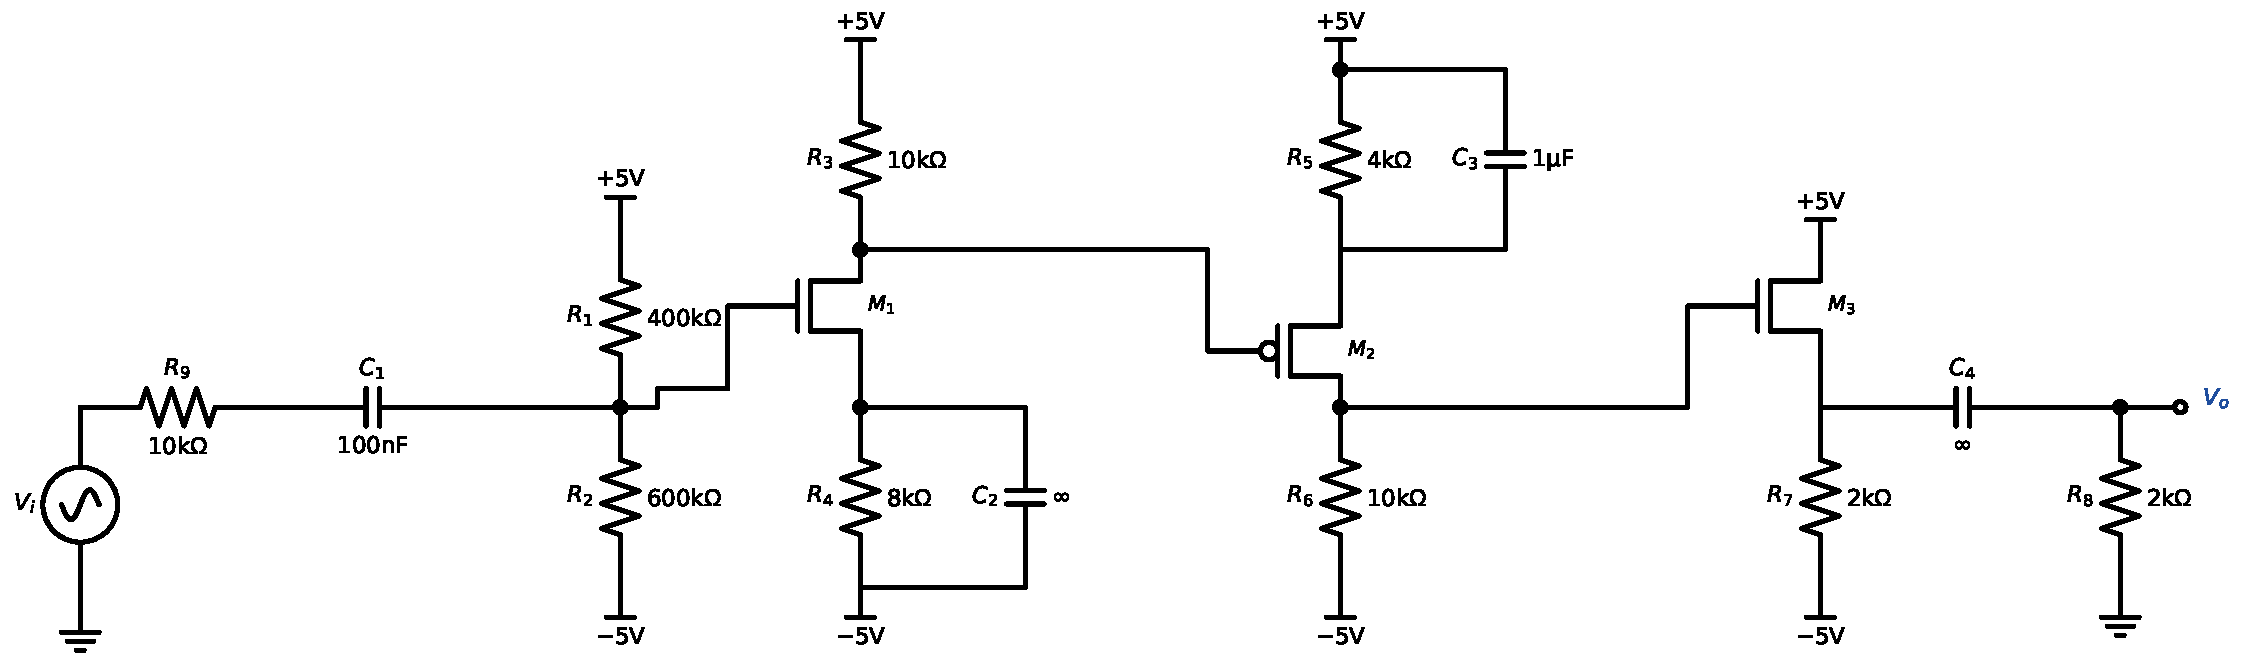
\includegraphics[width=0.9\linewidth,height=6cm,keepaspectratio]{p15_circuit}\end{center}
\solstep{1}{DC currents and transconductances}The DC drain currents are given: $I_{D1} = 461\,\mu \mathrm{A}$, $I_{D2} = 544\,\mu \mathrm{A}$, $I_{D3} = 1.26\,\mathrm{m}\mathrm{A}$. For AC every DC supply is ground and every ``$\infty$'' capacitor is a short. Transconductances (tool T4):\begin{align*}
g_{m1} &= k_{1}V_{ov1} = \sqrt{2k_{1}I_{D1}} = \sqrt{2\cdot1.1\,\mathrm{m}\mathrm{A/V^2}\cdot461\,\mu \mathrm{A}} = 1.01\,\mathrm{m}\mathrm{A/V},\qquad \frac{1}{g_{m1}} = 993\,\Omega\quad(V_{ov1} = 0.915\,\mathrm{V}) \\
g_{m2} &= k_{2}V_{ov2} = \sqrt{2k_{2}I_{D2}} = \sqrt{2\cdot850\,\mu \mathrm{A/V^2}\cdot544\,\mu \mathrm{A}} = 961\,\mu \mathrm{A/V},\qquad \frac{1}{g_{m2}} = 1.04\,\mathrm{k}\Omega\quad(V_{ov2} = 1.13\,\mathrm{V}) \\
g_{m3} &= k_{3}V_{ov3} = \sqrt{2k_{3}I_{D3}} = \sqrt{2\cdot1.1\,\mathrm{m}\mathrm{A/V^2}\cdot1.26\,\mathrm{m}\mathrm{A}} = 1.67\,\mathrm{m}\mathrm{A/V},\qquad \frac{1}{g_{m3}} = 600\,\Omega\quad(V_{ov3} = 1.51\,\mathrm{V})
\end{align*}

\solstep{2}{Input resistance of each stage}Input resistance of every stage, from the last back to the first (each one loads the stage before it):\begin{align*}
R_{i1} &= Z_{gate,1} = \infty\quad\text{(input at the gate: it loads nothing)} \\
R_{i2} &= Z_{gate,2} = \infty\quad\text{(input at the gate: it loads nothing)} \\
R_{i3} &= Z_{gate,3} = \infty\quad\text{(input at the gate: it loads nothing)}
\end{align*}

\solstep{3}{Gain along the signal path}Multiply the node-to-node gains along the signal path (tool T4):\[
H(s) = \frac{v_{g1}}{v_i}\cdot\frac{v_{d1}}{v_{g1}}\cdot\frac{v_{d2}}{v_{g2}}\cdot\frac{v_{s3}}{v_{g3}}
\]
\begin{align*}
\frac{v_{g1}}{v_i} &= \frac{R_{1} \parallel R_{2}}{R_{9} + \frac{1}{sC_{1}} + R_{1} \parallel R_{2}} = \dfrac{0.96\,s}{s + 40} \\
\frac{v_{d1}}{v_{g1}} &= -\frac{Z_{D1}}{1/g_{m1} + Z_{S1}},\quad Z_{D1} = R_{3},\ Z_{S1} = 0\ \Rightarrow\ -10.1 \\
\frac{v_{d2}}{v_{g2}} &= -\frac{Z_{D2}}{1/g_{m2} + Z_{S2}},\quad Z_{D2} = R_{6},\ Z_{S2} = R_{5} \parallel \frac{1}{sC_{3}}\ \Rightarrow\ \dfrac{-9.61\,s - 2400}{s + 1210} \\
\frac{v_{s3}}{v_{g3}} &= \frac{Z_{S3}}{1/g_{m3} + Z_{S3}},\quad Z_{S3} = R_{7} \parallel R_{8}\ \Rightarrow\ 0.625
\end{align*}

\solstep{4}{Transfer function}Multiply and simplify:\[
H(s) = \dfrac{58.1\,s^{2} + 14500\,s}{s^{2} + 1250\,s + 48500}
\]

\solstep{5}{Standard (Bode-ready) form}Find the roots. Every root $s=-p$ of the denominator is a \emph{pole}, every root $s=-z$ of the numerator is a \emph{zero}; $|p|$ and $|z|$ are the corner frequencies (rad/s).
\begin{itemize}[leftmargin=*,itemsep=2pt]
\item Numerator: it has the factor $s$ $\Rightarrow$ 1 zero at $s=0$.
\item Numerator (after taking out the $s$ factor): $58.1\,s + 14500$; divide by the leading coefficient $58.1$ (this does not move the roots): $s + 250$; $s + 250 = 0 \Rightarrow s = -250$.
\item Denominator: $s^{2} + 1250\,s + 48500$; quadratic formula:\[
s = \frac{-1250 \pm \sqrt{(1250)^2 - 4(48500)}}{2} = \frac{-1250 \pm 1170}{2} \Rightarrow s = -40,\ -1210
\]

\end{itemize}

Factored form (leading coefficient in front):
\[
H(s) = 58.1\,\dfrac{s(s+250)}{(s+40)(s+1210)}
\]

Bode-ready form: rewrite every $(s+p) = p\left(1+\frac{s}{p}\right)$ and $(s+z) = z\left(1+\frac{s}{z}\right)$, and collect all constants into $K$. Each $s$ in the numerator is paired with one of the \emph{lowest} poles as $\frac{s}{s+p}$ (that factor is $\approx 1$ above $p$). Then every factor except $K$ is $\approx 1$ inside the pass-band:
\[
H(s) = 12\,\dfrac{s}{s+2\pi\cdot 6.37}\,\left(1+\dfrac{s}{2\pi\cdot 39.8}\right)\,\dfrac{1}{1+\dfrac{s}{2\pi\cdot 193}},\qquad K = 12
\]

\begin{center}\renewcommand{\arraystretch}{1.35}
\begin{tabular}{cccc}
\toprule
type & $\omega_c$ (rad/s) & $f_c=\omega_c/2\pi$ & slope change \\
\midrule
pole & $40$ & 6.37 Hz & $-20$ dB/dec \\
zero & $250$ & 39.8 Hz & $+20$ dB/dec \\
pole & $1210$ & 193 Hz & $-20$ dB/dec \\
\bottomrule
\end{tabular}\end{center}

\solstep{6}{Magnitude Bode plot}Below every corner $|H(s)|\approx 0.3\,s$, so the plot starts with a slope of $+20$\,dB/dec. Then, moving right, each pole bends the line down by 20\,dB/dec and each zero bends it up by 20\,dB/dec (tool T6):
\begin{center}\renewcommand{\arraystretch}{1.35}
\begin{tabular}{lcl}
\toprule
frequency range & slope & asymptote level \\
\midrule
$f<$ 6.37 Hz & $+20$ dB/dec & 21.6 dB at end \\
6.37 Hz -- 39.8 Hz & $0$ dB/dec (flat) & 21.6 dB at start, 21.6 dB at end \\
39.8 Hz -- 193 Hz & $+20$ dB/dec & 21.6 dB at start, 35.3 dB at end \\
$f>$ 193 Hz & $0$ dB/dec (flat) & 35.3 dB at start \\
\bottomrule
\end{tabular}\end{center}

\begin{center}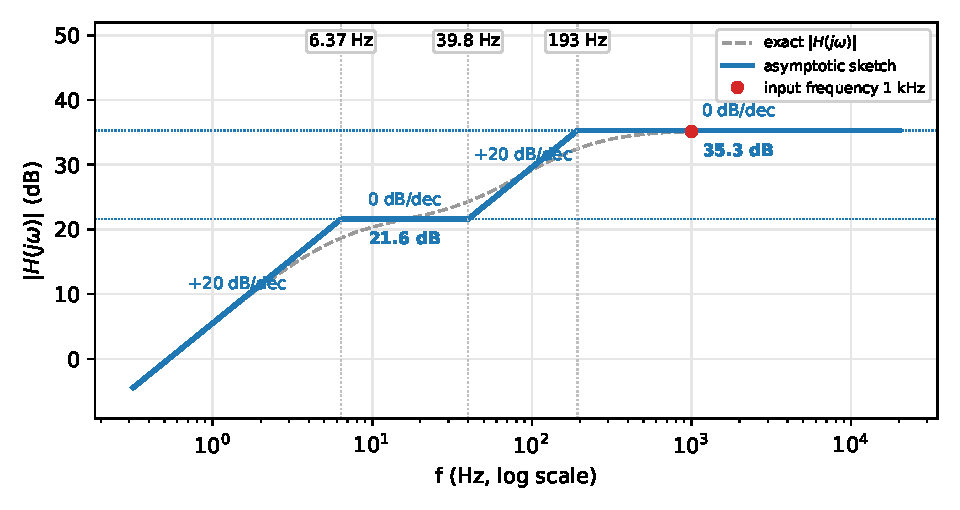
\includegraphics[width=0.78\linewidth,height=6.5cm,keepaspectratio]{p15_bode}\end{center}

{\small Blue: the straight-line sketch you are expected to draw. Dashed grey: the exact curve (about 3\,dB below the corner of an isolated pole). Red dot: the input frequency of Step 7.}
\solstep{7}{Steady-state output}The input is $V_i(t) = 0.001\sin\left(2\pi\cdot 1000\,t\right)$, so $\omega_{in} = 2\pi\cdot 1000 = 6280$\,rad/s. Put $s=j\omega_{in}$ in each factor (tool T5): magnitudes multiply, angles add.
{\small Rules: $\left|\frac{s}{s+p}\right| = \frac{\omega}{\sqrt{\omega^2+p^2}}$, $\angle = \frac{\pi}{2}-\tan^{-1}\frac{\omega}{p}$;\quad $\left|\frac{1}{1+s/p}\right| = \frac{1}{\sqrt{1+(\omega/p)^2}}$, $\angle = -\tan^{-1}\frac{\omega}{p}$;\quad $\left|1+\frac{s}{z}\right| = \sqrt{1+(\omega/z)^2}$, $\angle = \tan^{-1}\frac{\omega}{z}$;\quad a negative $K$ adds $-\pi$.}
\begin{center}\renewcommand{\arraystretch}{1.35}
\begin{tabular}{ccc}
\toprule
factor & magnitude & angle (rad) \\
\midrule
$12$ & $11.98$ & $0$ \\
$\rule[-1.1em]{0pt}{2.8em}\dfrac{s}{s+2\pi\cdot 6.37}$ & $1$ & $0.00637$ \\
$\rule[-1.1em]{0pt}{2.8em}\left(1+\dfrac{s}{2\pi\cdot 39.8}\right)$ & $25.15$ & $1.53$ \\
$\rule[-1.7em]{0pt}{4em}\dfrac{1}{1+\dfrac{s}{2\pi\cdot 193}}$ & $0.1893$ & $-1.38$ \\
\textbf{total} & $\mathbf{57.05}$ (product) & $\mathbf{0.157}$ (sum) \\
\bottomrule
\end{tabular}\end{center}

\begin{align*}
|H(j\omega_{in})| &= 57.1, \qquad \angle H(j\omega_{in}) = 0.157\ \mathrm{rad} \\
v_{o,ac}(t) &= 57.1\times 0.001\,\sin\left(2\pi\cdot 1000\,t + 0.157\right) = 0.0571\,\sin\left(2\pi\cdot 1000\,t + 0.157\right)
\end{align*}

\[
\boxed{V_o(t) = 0.0571\,\sin\left(2\pi\cdot 1000\,t + 0.157\right)\ \mathrm{V}}
\]

\begin{ansbox}
$H(s) = 12\,\dfrac{s}{s+2\pi\cdot 6.37}\,\left(1+\dfrac{s}{2\pi\cdot 39.8}\right)\,\dfrac{1}{1+\dfrac{s}{2\pi\cdot 193}}$\quad (corners: 6.37 Hz, 39.8 Hz, 193 Hz)\\[4pt]
$V_o(t) = 0.0571\,\sin\left(2\pi\cdot 1000\,t + 0.157\right)\ \mathrm{V}$
\end{ansbox}

\newpage
\subsection*{Solution 5D.16 \hfill Hard}
\begin{center}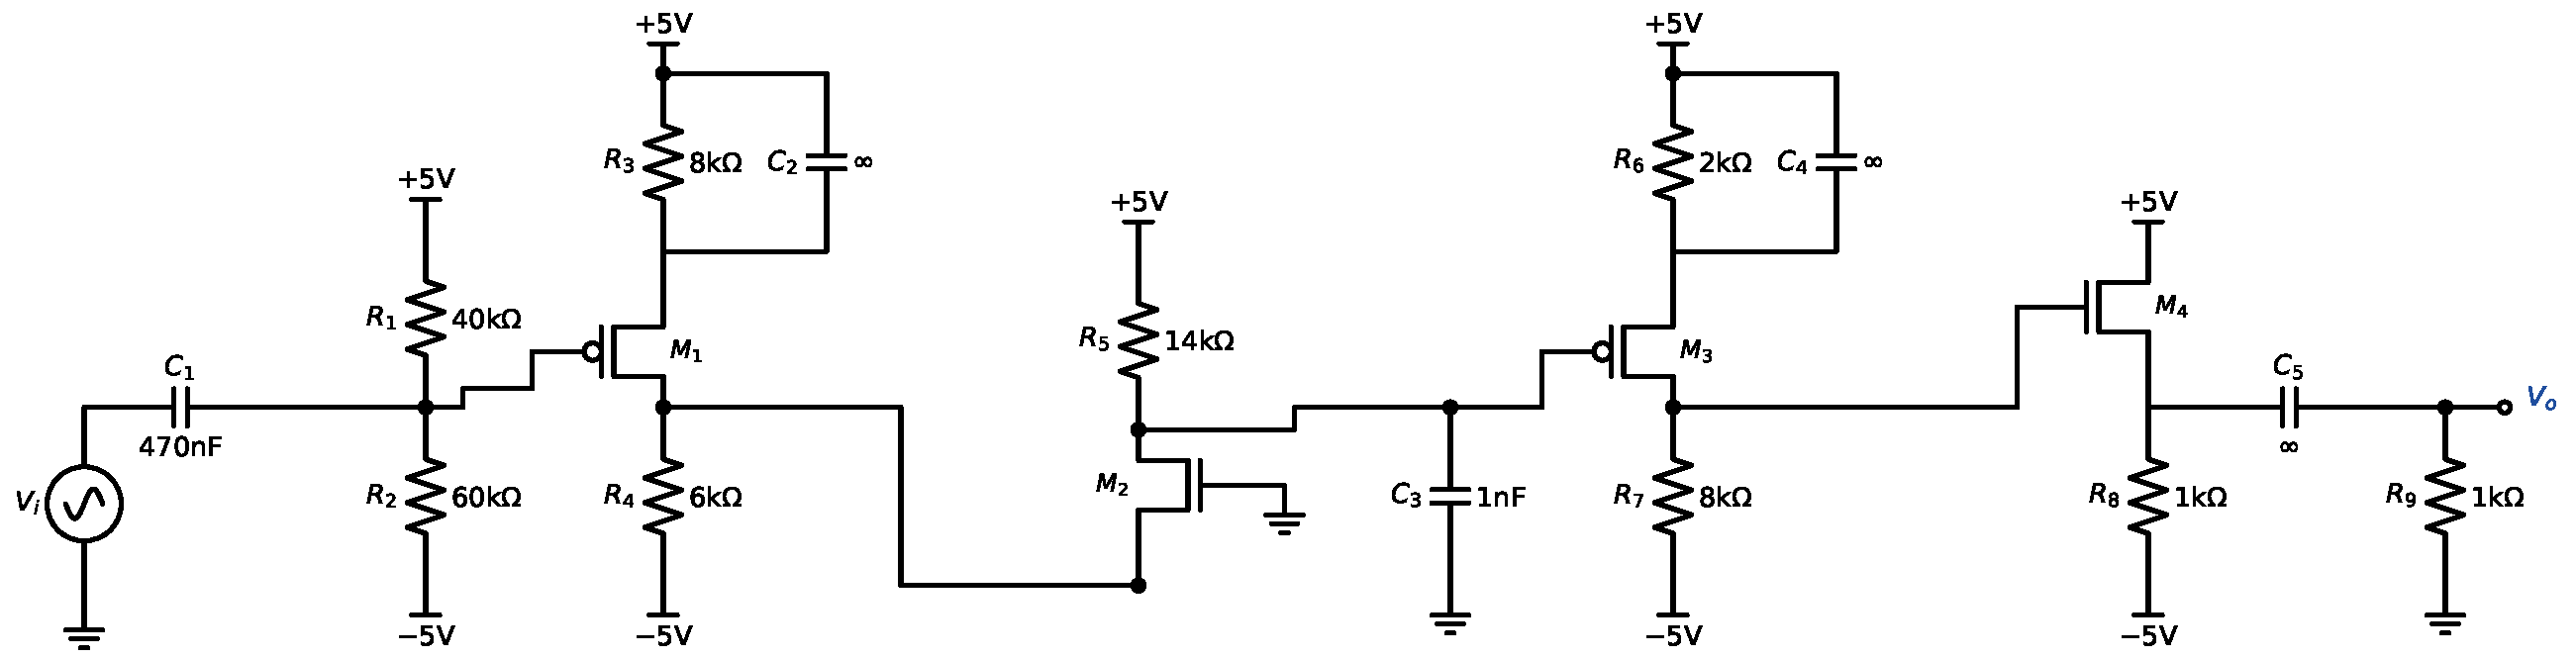
\includegraphics[width=0.9\linewidth,height=6cm,keepaspectratio]{p16_circuit}\end{center}
\solstep{1}{DC currents and transconductances}The DC drain currents are given: $I_{D1} = 243\,\mu \mathrm{A}$, $I_{D2} = 246\,\mu \mathrm{A}$, $I_{D3} = 518\,\mu \mathrm{A}$, $I_{D4} = 1.24\,\mathrm{m}\mathrm{A}$. For AC every DC supply is ground and every ``$\infty$'' capacitor is a short. Transconductances (tool T4):\begin{align*}
g_{m1} &= k_{1}V_{ov1} = \sqrt{2k_{1}I_{D1}} = \sqrt{2\cdot850\,\mu \mathrm{A/V^2}\cdot243\,\mu \mathrm{A}} = 643\,\mu \mathrm{A/V},\qquad \frac{1}{g_{m1}} = 1.56\,\mathrm{k}\Omega\quad(V_{ov1} = 0.756\,\mathrm{V}) \\
g_{m2} &= k_{2}V_{ov2} = \sqrt{2k_{2}I_{D2}} = \sqrt{2\cdot1.1\,\mathrm{m}\mathrm{A/V^2}\cdot246\,\mu \mathrm{A}} = 735\,\mu \mathrm{A/V},\qquad \frac{1}{g_{m2}} = 1.36\,\mathrm{k}\Omega\quad(V_{ov2} = 0.668\,\mathrm{V}) \\
g_{m3} &= k_{3}V_{ov3} = \sqrt{2k_{3}I_{D3}} = \sqrt{2\cdot850\,\mu \mathrm{A/V^2}\cdot518\,\mu \mathrm{A}} = 938\,\mu \mathrm{A/V},\qquad \frac{1}{g_{m3}} = 1.07\,\mathrm{k}\Omega\quad(V_{ov3} = 1.1\,\mathrm{V}) \\
g_{m4} &= k_{4}V_{ov4} = \sqrt{2k_{4}I_{D4}} = \sqrt{2\cdot1.1\,\mathrm{m}\mathrm{A/V^2}\cdot1.24\,\mathrm{m}\mathrm{A}} = 1.65\,\mathrm{m}\mathrm{A/V},\qquad \frac{1}{g_{m4}} = 606\,\Omega\quad(V_{ov4} = 1.5\,\mathrm{V})
\end{align*}

\solstep{2}{Input resistance of each stage}Input resistance of every stage, from the last back to the first (each one loads the stage before it):\begin{align*}
R_{i1} &= Z_{gate,1} = \infty\quad\text{(input at the gate: it loads nothing)} \\
R_{i2} &= Z_{source,2} = \frac{1}{g_{m2}} = 1.36\,\mathrm{k}\Omega\quad\text{(common gate)} \\
R_{i3} &= Z_{gate,3} = \infty\quad\text{(input at the gate: it loads nothing)} \\
R_{i4} &= Z_{gate,4} = \infty\quad\text{(input at the gate: it loads nothing)}
\end{align*}

\solstep{3}{Gain along the signal path}Multiply the node-to-node gains along the signal path (tool T4):\[
H(s) = \frac{v_{g1}}{v_i}\cdot\frac{v_{d1}}{v_{g1}}\cdot\frac{v_{d2}}{v_{s2}}\cdot\frac{v_{d3}}{v_{g3}}\cdot\frac{v_{s4}}{v_{g4}}
\]
\begin{align*}
\frac{v_{g1}}{v_i} &= \frac{R_{1} \parallel R_{2}}{\frac{1}{sC_{1}} + R_{1} \parallel R_{2}} = \dfrac{s}{s + 88.7} \\
\frac{v_{d1}}{v_{g1}} &= -\frac{Z_{D1}}{1/g_{m1} + Z_{S1}},\quad Z_{D1} = R_{4} \parallel R_{i2},\ Z_{S1} = 0\ \Rightarrow\ -0.713 \\
\frac{v_{d2}}{v_{s2}} &= \frac{Z_{D2}}{1/g_{m2}},\quad Z_{D2} = R_{5} \parallel \frac{1}{sC_{3}}\ \Rightarrow\ \dfrac{7.35\times 10^{5}}{s + 71400} \\
\frac{v_{d3}}{v_{g3}} &= -\frac{Z_{D3}}{1/g_{m3} + Z_{S3}},\quad Z_{D3} = R_{7},\ Z_{S3} = 0\ \Rightarrow\ -7.5 \\
\frac{v_{s4}}{v_{g4}} &= \frac{Z_{S4}}{1/g_{m4} + Z_{S4}},\quad Z_{S4} = R_{8} \parallel R_{9}\ \Rightarrow\ 0.452
\end{align*}

\solstep{4}{Transfer function}Multiply and simplify:\[
H(s) = \dfrac{1.78\times 10^{6}\,s}{s^{2} + 71500\,s + 6.33\times 10^{6}}
\]

\solstep{5}{Standard (Bode-ready) form}Find the roots. Every root $s=-p$ of the denominator is a \emph{pole}, every root $s=-z$ of the numerator is a \emph{zero}; $|p|$ and $|z|$ are the corner frequencies (rad/s).
\begin{itemize}[leftmargin=*,itemsep=2pt]
\item Numerator: it has the factor $s$ $\Rightarrow$ 1 zero at $s=0$.
\item Denominator: $s^{2} + 71500\,s + 6.33\times 10^{6}$; quadratic formula:\[
s = \frac{-71500 \pm \sqrt{(71500)^2 - 4(6.33\times 10^{6})}}{2} = \frac{-71500 \pm 71300}{2} \Rightarrow s = -88.7,\ -71400
\]

\end{itemize}

Factored form (leading coefficient in front):
\[
H(s) = 1.78\times 10^{6}\,\dfrac{s}{(s+88.7)(s+71400)}
\]

Bode-ready form: rewrite every $(s+p) = p\left(1+\frac{s}{p}\right)$ and $(s+z) = z\left(1+\frac{s}{z}\right)$, and collect all constants into $K$. Each $s$ in the numerator is paired with one of the \emph{lowest} poles as $\frac{s}{s+p}$ (that factor is $\approx 1$ above $p$). Then every factor except $K$ is $\approx 1$ inside the pass-band:
\[
H(s) = 24.9\,\dfrac{s}{s+2\pi\cdot 14.1}\,\dfrac{1}{1+\dfrac{s}{2\pi\cdot 11.4\mathrm{k}}},\qquad K = 24.9
\]

\begin{center}\renewcommand{\arraystretch}{1.35}
\begin{tabular}{cccc}
\toprule
type & $\omega_c$ (rad/s) & $f_c=\omega_c/2\pi$ & slope change \\
\midrule
pole & $88.7$ & 14.1 Hz & $-20$ dB/dec \\
pole & $71400$ & 11.4 kHz & $-20$ dB/dec \\
\bottomrule
\end{tabular}\end{center}

\solstep{6}{Magnitude Bode plot}Below every corner $|H(s)|\approx 0.281\,s$, so the plot starts with a slope of $+20$\,dB/dec. Then, moving right, each pole bends the line down by 20\,dB/dec and each zero bends it up by 20\,dB/dec (tool T6):
\begin{center}\renewcommand{\arraystretch}{1.35}
\begin{tabular}{lcl}
\toprule
frequency range & slope & asymptote level \\
\midrule
$f<$ 14.1 Hz & $+20$ dB/dec & 27.9 dB at end \\
14.1 Hz -- 11.4 kHz & $0$ dB/dec (flat) & 27.9 dB at start, 27.9 dB at end \\
$f>$ 11.4 kHz & $-20$ dB/dec & 27.9 dB at start \\
\bottomrule
\end{tabular}\end{center}

The flat (pass-band) level is $20\log_{10}|K| = 20\log_{10}24.9 = 27.9$\,dB.
\begin{center}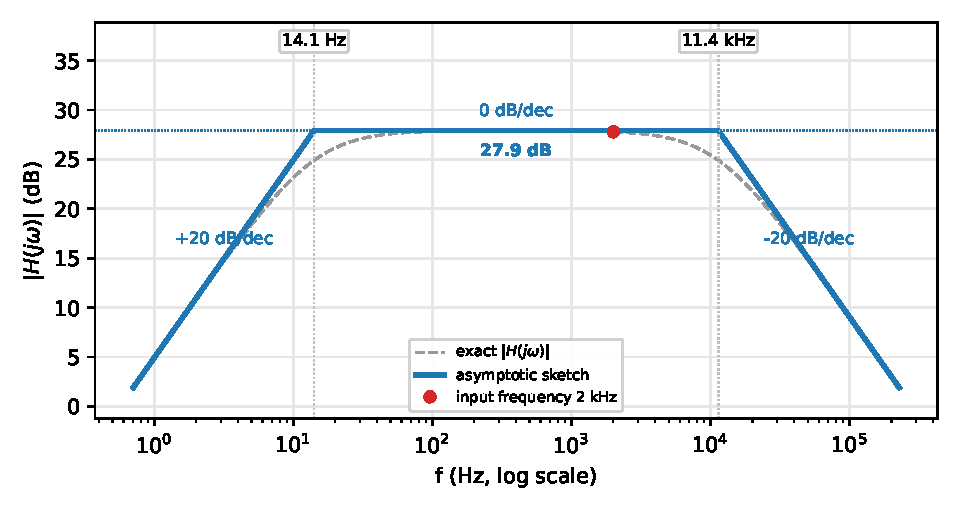
\includegraphics[width=0.78\linewidth,height=6.5cm,keepaspectratio]{p16_bode}\end{center}

{\small Blue: the straight-line sketch you are expected to draw. Dashed grey: the exact curve (about 3\,dB below the corner of an isolated pole). Red dot: the input frequency of Step 7.}
\solstep{7}{Steady-state output}The input is $V_i(t) = 0.001\sin\left(2\pi\cdot 2000\,t\right)$, so $\omega_{in} = 2\pi\cdot 2000 = 12600$\,rad/s. Put $s=j\omega_{in}$ in each factor (tool T5): magnitudes multiply, angles add.
{\small Rules: $\left|\frac{s}{s+p}\right| = \frac{\omega}{\sqrt{\omega^2+p^2}}$, $\angle = \frac{\pi}{2}-\tan^{-1}\frac{\omega}{p}$;\quad $\left|\frac{1}{1+s/p}\right| = \frac{1}{\sqrt{1+(\omega/p)^2}}$, $\angle = -\tan^{-1}\frac{\omega}{p}$;\quad $\left|1+\frac{s}{z}\right| = \sqrt{1+(\omega/z)^2}$, $\angle = \tan^{-1}\frac{\omega}{z}$;\quad a negative $K$ adds $-\pi$.}
\begin{center}\renewcommand{\arraystretch}{1.35}
\begin{tabular}{ccc}
\toprule
factor & magnitude & angle (rad) \\
\midrule
$24.9$ & $24.9$ & $0$ \\
$\rule[-1.1em]{0pt}{2.8em}\dfrac{s}{s+2\pi\cdot 14.1}$ & $1$ & $0.00705$ \\
$\rule[-1.7em]{0pt}{4em}\dfrac{1}{1+\dfrac{s}{2\pi\cdot 11.4\mathrm{k}}}$ & $0.9849$ & $-0.174$ \\
\textbf{total} & $\mathbf{24.52}$ (product) & $\mathbf{-0.167}$ (sum) \\
\bottomrule
\end{tabular}\end{center}

\begin{align*}
|H(j\omega_{in})| &= 24.5, \qquad \angle H(j\omega_{in}) = -0.167\ \mathrm{rad} \\
v_{o,ac}(t) &= 24.5\times 0.001\,\sin\left(2\pi\cdot 2000\,t - 0.167\right) = 0.0245\,\sin\left(2\pi\cdot 2000\,t - 0.167\right)
\end{align*}

\[
\boxed{V_o(t) = 0.0245\,\sin\left(2\pi\cdot 2000\,t - 0.167\right)\ \mathrm{V}}
\]

\begin{ansbox}
$H(s) = 24.9\,\dfrac{s}{s+2\pi\cdot 14.1}\,\dfrac{1}{1+\dfrac{s}{2\pi\cdot 11.4\mathrm{k}}}$\quad (corners: 14.1 Hz, 11.4 kHz)\\[4pt]
$V_o(t) = 0.0245\,\sin\left(2\pi\cdot 2000\,t - 0.167\right)\ \mathrm{V}$
\end{ansbox}

\newpage
\subsection*{Solution 5D.17 \hfill Hard}
\begin{center}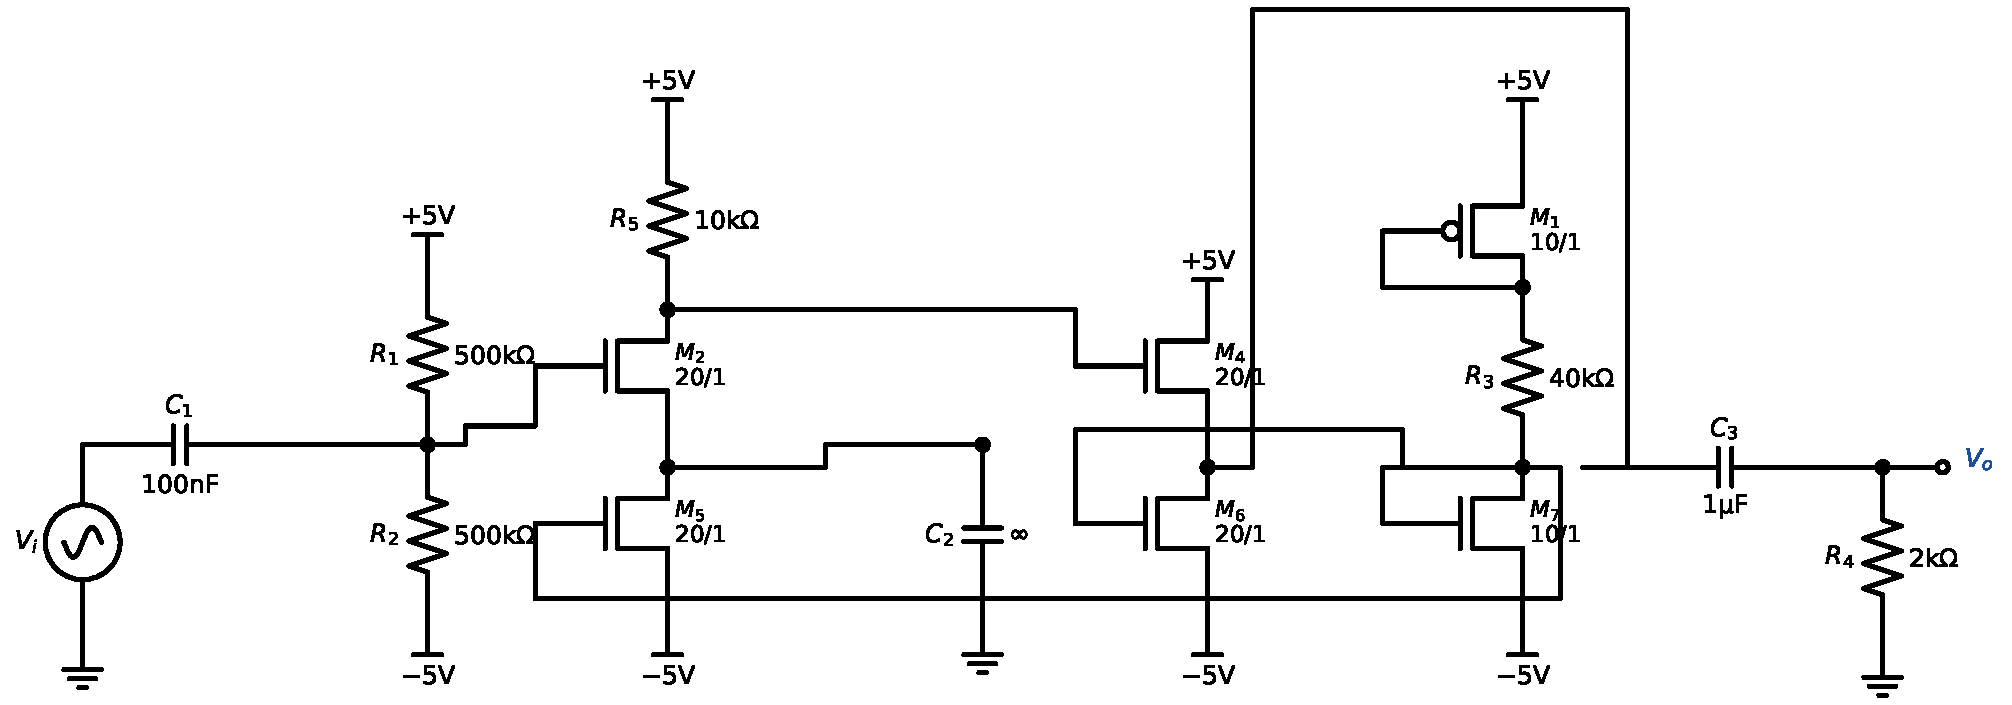
\includegraphics[width=0.9\linewidth,height=6cm,keepaspectratio]{p17_circuit}\end{center}
\solstep{1}{DC currents and transconductances}The DC drain currents are given: $I_{D2} = 373\,\mu \mathrm{A}$, $I_{D4} = 373\,\mu \mathrm{A}$. For AC every DC supply is ground and every ``$\infty$'' capacitor is a short. Transconductances (tool T4):\begin{align*}
g_{m2} &= k_{2}V_{ov2} = \sqrt{2k_{2}I_{D2}} = \sqrt{2\cdot4\,\mathrm{m}\mathrm{A/V^2}\cdot373\,\mu \mathrm{A}} = 1.73\,\mathrm{m}\mathrm{A/V},\qquad \frac{1}{g_{m2}} = 579\,\Omega\quad(V_{ov2} = 0.432\,\mathrm{V}) \\
g_{m4} &= k_{4}V_{ov4} = \sqrt{2k_{4}I_{D4}} = \sqrt{2\cdot4\,\mathrm{m}\mathrm{A/V^2}\cdot373\,\mu \mathrm{A}} = 1.73\,\mathrm{m}\mathrm{A/V},\qquad \frac{1}{g_{m4}} = 579\,\Omega\quad(V_{ov4} = 0.432\,\mathrm{V})
\end{align*}

\solstep{2}{Input resistance of each stage}Input resistance of every stage, from the last back to the first (each one loads the stage before it):\begin{align*}
R_{i2} &= Z_{gate,2} = \infty\quad\text{(input at the gate: it loads nothing)} \\
R_{i4} &= Z_{gate,4} = \infty\quad\text{(input at the gate: it loads nothing)}
\end{align*}

\solstep{3}{Gain along the signal path}Multiply the node-to-node gains along the signal path (tool T4):\[
H(s) = \frac{v_{g2}}{v_i}\cdot\frac{v_{d2}}{v_{g2}}\cdot\frac{v_{s4}}{v_{g4}}\cdot\frac{v_o}{v_{s4}}
\]
\begin{align*}
\frac{v_{g2}}{v_i} &= \frac{R_{1} \parallel R_{2}}{\frac{1}{sC_{1}} + R_{1} \parallel R_{2}} = \dfrac{s}{s + 40} \\
\frac{v_{d2}}{v_{g2}} &= -\frac{Z_{D2}}{1/g_{m2} + Z_{S2}},\quad Z_{D2} = R_{5},\ Z_{S2} = 0\ \Rightarrow\ -17.3 \\
\frac{v_{s4}}{v_{g4}} &= \frac{Z_{S4}}{1/g_{m4} + Z_{S4}},\quad Z_{S4} = \frac{1}{sC_{3}} + R_{4}\ \Rightarrow\ \dfrac{0.775\,s + 388}{s + 388} \\
\frac{v_o}{v_{s4}} &= \frac{R_{4}}{\frac{1}{sC_{3}} + R_{4}} = \dfrac{s}{s + 500}
\end{align*}

\solstep{4}{Transfer function}Multiply and simplify:\[
H(s) = \dfrac{-13.4\,s^{2}}{s^{2} + 428\,s + 15500}
\]

\solstep{5}{Standard (Bode-ready) form}Find the roots. Every root $s=-p$ of the denominator is a \emph{pole}, every root $s=-z$ of the numerator is a \emph{zero}; $|p|$ and $|z|$ are the corner frequencies (rad/s).
\begin{itemize}[leftmargin=*,itemsep=2pt]
\item Numerator: it has the factor $s^2$ $\Rightarrow$ 2 zeros at $s=0$.
\item Denominator: $s^{2} + 428\,s + 15500$; quadratic formula:\[
s = \frac{-428 \pm \sqrt{(428)^2 - 4(15500)}}{2} = \frac{-428 \pm 348}{2} \Rightarrow s = -40,\ -388
\]

\end{itemize}

Factored form (leading coefficient in front):
\[
H(s) = -13.4\,\dfrac{s^{2}}{(s+40)(s+388)}
\]

Bode-ready form: rewrite every $(s+p) = p\left(1+\frac{s}{p}\right)$ and $(s+z) = z\left(1+\frac{s}{z}\right)$, and collect all constants into $K$. Each $s$ in the numerator is paired with one of the \emph{lowest} poles as $\frac{s}{s+p}$ (that factor is $\approx 1$ above $p$). Then every factor except $K$ is $\approx 1$ inside the pass-band:
\[
H(s) = -13.4\,\dfrac{s}{s+2\pi\cdot 6.37}\,\dfrac{s}{s+2\pi\cdot 61.7},\qquad K = -13.4
\]

\begin{center}\renewcommand{\arraystretch}{1.35}
\begin{tabular}{cccc}
\toprule
type & $\omega_c$ (rad/s) & $f_c=\omega_c/2\pi$ & slope change \\
\midrule
pole & $40$ & 6.37 Hz & $-20$ dB/dec \\
pole & $388$ & 61.7 Hz & $-20$ dB/dec \\
\bottomrule
\end{tabular}\end{center}

\solstep{6}{Magnitude Bode plot}Below every corner $|H(s)|\approx 8.64\times 10^{-4}\,s^2$, so the plot starts with a slope of $+40$\,dB/dec. Then, moving right, each pole bends the line down by 20\,dB/dec and each zero bends it up by 20\,dB/dec (tool T6):
\begin{center}\renewcommand{\arraystretch}{1.35}
\begin{tabular}{lcl}
\toprule
frequency range & slope & asymptote level \\
\midrule
$f<$ 6.37 Hz & $+40$ dB/dec & 2.81 dB at end \\
6.37 Hz -- 61.7 Hz & $+20$ dB/dec & 2.81 dB at start, 22.5 dB at end \\
$f>$ 61.7 Hz & $0$ dB/dec (flat) & 22.5 dB at start \\
\bottomrule
\end{tabular}\end{center}

The flat (pass-band) level is $20\log_{10}|K| = 20\log_{10}13.4 = 22.5$\,dB.
\begin{center}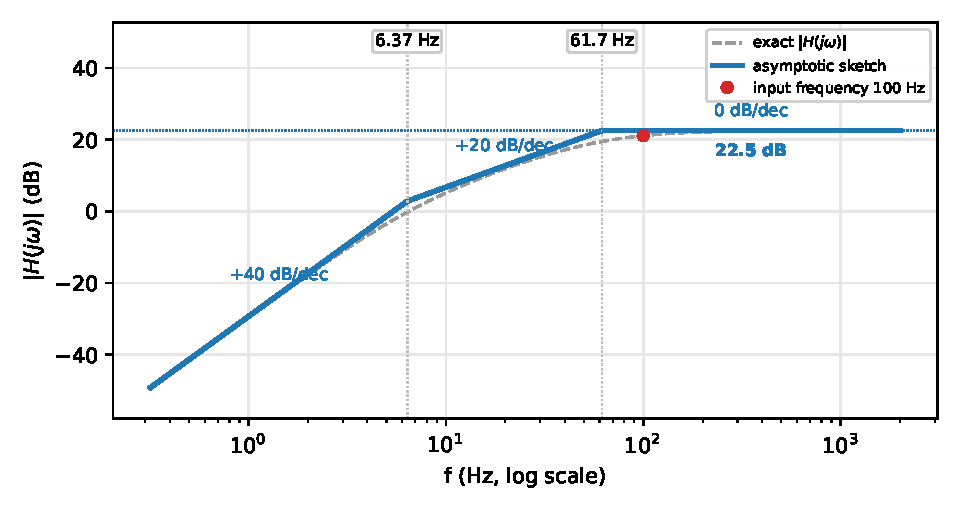
\includegraphics[width=0.78\linewidth,height=6.5cm,keepaspectratio]{p17_bode}\end{center}

{\small Blue: the straight-line sketch you are expected to draw. Dashed grey: the exact curve (about 3\,dB below the corner of an isolated pole). Red dot: the input frequency of Step 7.}
\solstep{7}{Steady-state output}The input is $V_i(t) = 0.01\sin\left(2\pi\cdot 100\,t\right)$, so $\omega_{in} = 2\pi\cdot 100 = 628$\,rad/s. Put $s=j\omega_{in}$ in each factor (tool T5): magnitudes multiply, angles add.
{\small Rules: $\left|\frac{s}{s+p}\right| = \frac{\omega}{\sqrt{\omega^2+p^2}}$, $\angle = \frac{\pi}{2}-\tan^{-1}\frac{\omega}{p}$;\quad $\left|\frac{1}{1+s/p}\right| = \frac{1}{\sqrt{1+(\omega/p)^2}}$, $\angle = -\tan^{-1}\frac{\omega}{p}$;\quad $\left|1+\frac{s}{z}\right| = \sqrt{1+(\omega/z)^2}$, $\angle = \tan^{-1}\frac{\omega}{z}$;\quad a negative $K$ adds $-\pi$.}
\begin{center}\renewcommand{\arraystretch}{1.35}
\begin{tabular}{ccc}
\toprule
factor & magnitude & angle (rad) \\
\midrule
$-13.4$ & $13.39$ & $-3.14$ \\
$\rule[-1.1em]{0pt}{2.8em}\dfrac{s}{s+2\pi\cdot 6.37}$ & $0.998$ & $0.0636$ \\
$\rule[-1.1em]{0pt}{2.8em}\dfrac{s}{s+2\pi\cdot 61.7}$ & $0.851$ & $0.553$ \\
\textbf{total} & $\mathbf{11.38}$ (product) & $\mathbf{-2.53}$ (sum) \\
\bottomrule
\end{tabular}\end{center}

\begin{align*}
|H(j\omega_{in})| &= 11.4, \qquad \angle H(j\omega_{in}) = -2.53\ \mathrm{rad} \\
v_{o,ac}(t) &= 11.4\times 0.01\,\sin\left(2\pi\cdot 100\,t - 2.53\right) = 0.114\,\sin\left(2\pi\cdot 100\,t - 2.53\right)
\end{align*}

\[
\boxed{V_o(t) = 0.114\,\sin\left(2\pi\cdot 100\,t - 2.53\right)\ \mathrm{V}}
\]

\begin{ansbox}
$H(s) = -13.4\,\dfrac{s}{s+2\pi\cdot 6.37}\,\dfrac{s}{s+2\pi\cdot 61.7}$\quad (corners: 6.37 Hz, 61.7 Hz)\\[4pt]
$V_o(t) = 0.114\,\sin\left(2\pi\cdot 100\,t - 2.53\right)\ \mathrm{V}$
\end{ansbox}

\newpage
\subsection*{Solution 5D.18 \hfill Hard}
\begin{center}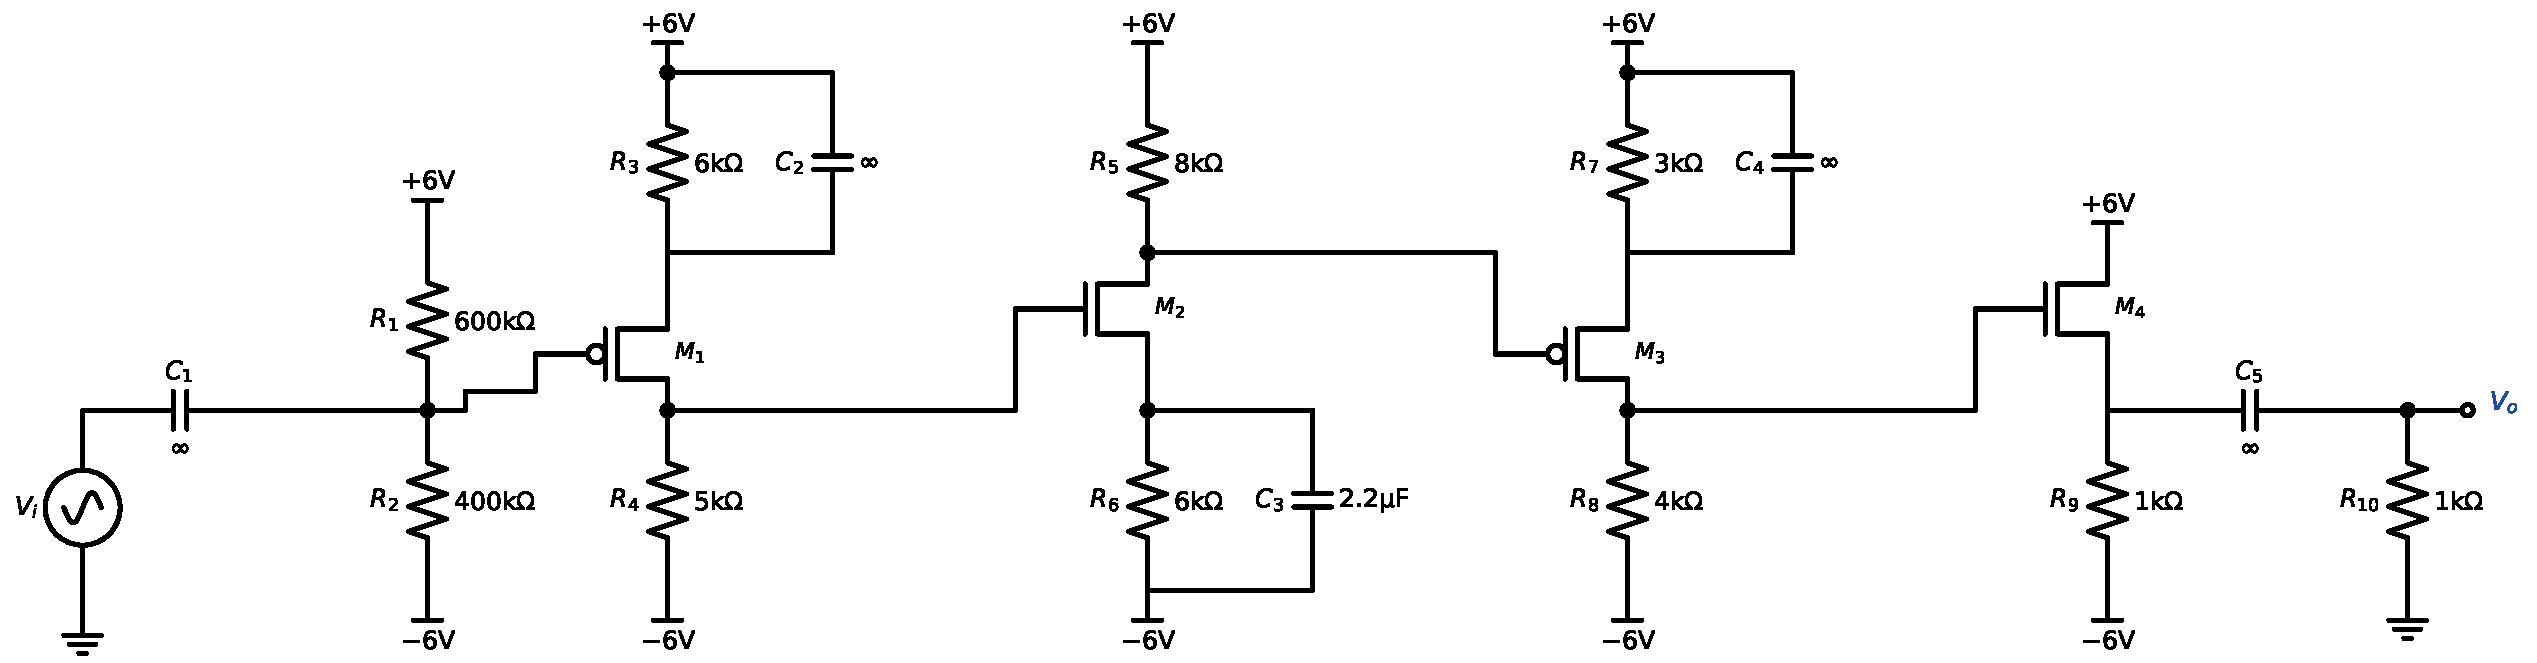
\includegraphics[width=0.9\linewidth,height=6cm,keepaspectratio]{p18_circuit}\end{center}
\solstep{1}{DC currents and transconductances}The DC drain currents are given: $I_{D1} = 820\,\mu \mathrm{A}$, $I_{D2} = 410\,\mu \mathrm{A}$, $I_{D3} = 445\,\mu \mathrm{A}$, $I_{D4} = 265\,\mu \mathrm{A}$. For AC every DC supply is ground and every ``$\infty$'' capacitor is a short. Transconductances (tool T4):\begin{align*}
g_{m1} &= k_{1}V_{ov1} = \sqrt{2k_{1}I_{D1}} = \sqrt{2\cdot1\,\mathrm{m}\mathrm{A/V^2}\cdot820\,\mu \mathrm{A}} = 1.28\,\mathrm{m}\mathrm{A/V},\qquad \frac{1}{g_{m1}} = 781\,\Omega\quad(V_{ov1} = 1.28\,\mathrm{V}) \\
g_{m2} &= k_{2}V_{ov2} = \sqrt{2k_{2}I_{D2}} = \sqrt{2\cdot2\,\mathrm{m}\mathrm{A/V^2}\cdot410\,\mu \mathrm{A}} = 1.28\,\mathrm{m}\mathrm{A/V},\qquad \frac{1}{g_{m2}} = 781\,\Omega\quad(V_{ov2} = 0.64\,\mathrm{V}) \\
g_{m3} &= k_{3}V_{ov3} = \sqrt{2k_{3}I_{D3}} = \sqrt{2\cdot1\,\mathrm{m}\mathrm{A/V^2}\cdot445\,\mu \mathrm{A}} = 944\,\mu \mathrm{A/V},\qquad \frac{1}{g_{m3}} = 1.06\,\mathrm{k}\Omega\quad(V_{ov3} = 0.944\,\mathrm{V}) \\
g_{m4} &= k_{4}V_{ov4} = \sqrt{2k_{4}I_{D4}} = \sqrt{2\cdot2\,\mathrm{m}\mathrm{A/V^2}\cdot265\,\mu \mathrm{A}} = 1.03\,\mathrm{m}\mathrm{A/V},\qquad \frac{1}{g_{m4}} = 970\,\Omega\quad(V_{ov4} = 0.515\,\mathrm{V})
\end{align*}

\solstep{2}{Input resistance of each stage}Input resistance of every stage, from the last back to the first (each one loads the stage before it):\begin{align*}
R_{i1} &= Z_{gate,1} = \infty\quad\text{(input at the gate: it loads nothing)} \\
R_{i2} &= Z_{gate,2} = \infty\quad\text{(input at the gate: it loads nothing)} \\
R_{i3} &= Z_{gate,3} = \infty\quad\text{(input at the gate: it loads nothing)} \\
R_{i4} &= Z_{gate,4} = \infty\quad\text{(input at the gate: it loads nothing)}
\end{align*}

\solstep{3}{Gain along the signal path}Multiply the node-to-node gains along the signal path (tool T4):\[
H(s) = \frac{v_{d1}}{v_{g1}}\cdot\frac{v_{d2}}{v_{g2}}\cdot\frac{v_{d3}}{v_{g3}}\cdot\frac{v_{s4}}{v_{g4}}
\]
\begin{align*}
\frac{v_{d1}}{v_{g1}} &= -\frac{Z_{D1}}{1/g_{m1} + Z_{S1}},\quad Z_{D1} = R_{4},\ Z_{S1} = 0\ \Rightarrow\ -6.4 \\
\frac{v_{d2}}{v_{g2}} &= -\frac{Z_{D2}}{1/g_{m2} + Z_{S2}},\quad Z_{D2} = R_{5},\ Z_{S2} = R_{6} \parallel \frac{1}{sC_{3}}\ \Rightarrow\ \dfrac{-10.2\,s - 776}{s + 658} \\
\frac{v_{d3}}{v_{g3}} &= -\frac{Z_{D3}}{1/g_{m3} + Z_{S3}},\quad Z_{D3} = R_{8},\ Z_{S3} = 0\ \Rightarrow\ -3.77 \\
\frac{v_{s4}}{v_{g4}} &= \frac{Z_{S4}}{1/g_{m4} + Z_{S4}},\quad Z_{S4} = R_{9} \parallel R_{10}\ \Rightarrow\ 0.34
\end{align*}

\solstep{4}{Transfer function}Multiply and simplify:\[
H(s) = \dfrac{-84.2\,s - 6380}{s + 658}
\]

\solstep{5}{Standard (Bode-ready) form}Find the roots. Every root $s=-p$ of the denominator is a \emph{pole}, every root $s=-z$ of the numerator is a \emph{zero}; $|p|$ and $|z|$ are the corner frequencies (rad/s).
\begin{itemize}[leftmargin=*,itemsep=2pt]
\item Numerator: $-84.2\,s - 6380$; divide by the leading coefficient $-84.2$ (this does not move the roots): $s + 75.8$; $s + 75.8 = 0 \Rightarrow s = -75.8$.
\item Denominator: $s + 658$; $s + 658 = 0 \Rightarrow s = -658$.
\end{itemize}

Factored form (leading coefficient in front):
\[
H(s) = -84.2\,\dfrac{(s+75.8)}{(s+658)}
\]

Bode-ready form: rewrite every $(s+p) = p\left(1+\frac{s}{p}\right)$ and $(s+z) = z\left(1+\frac{s}{z}\right)$, and collect all constants into $K$. Then every factor except $K$ is $\approx 1$ inside the pass-band:
\[
H(s) = -9.69\,\left(1+\dfrac{s}{2\pi\cdot 12.1}\right)\,\dfrac{1}{1+\dfrac{s}{2\pi\cdot 105}},\qquad K = -9.69
\]

\begin{center}\renewcommand{\arraystretch}{1.35}
\begin{tabular}{cccc}
\toprule
type & $\omega_c$ (rad/s) & $f_c=\omega_c/2\pi$ & slope change \\
\midrule
zero & $75.8$ & 12.1 Hz & $+20$ dB/dec \\
pole & $658$ & 105 Hz & $-20$ dB/dec \\
\bottomrule
\end{tabular}\end{center}

\solstep{6}{Magnitude Bode plot}Below every corner, all factors are $\approx$ constant: $|H| \approx 9.69$ $= 19.7$\,dB (flat, 0 dB/dec). Then, moving right, each pole bends the line down by 20\,dB/dec and each zero bends it up by 20\,dB/dec (tool T6):
\begin{center}\renewcommand{\arraystretch}{1.35}
\begin{tabular}{lcl}
\toprule
frequency range & slope & asymptote level \\
\midrule
$f<$ 12.1 Hz & $0$ dB/dec (flat) & 19.7 dB at end \\
12.1 Hz -- 105 Hz & $+20$ dB/dec & 19.7 dB at start, 38.5 dB at end \\
$f>$ 105 Hz & $0$ dB/dec (flat) & 38.5 dB at start \\
\bottomrule
\end{tabular}\end{center}

\begin{center}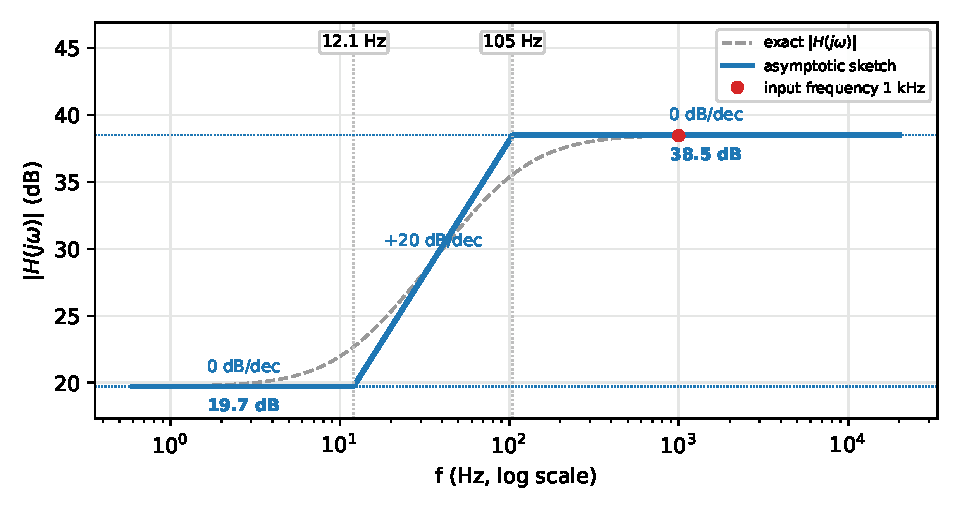
\includegraphics[width=0.78\linewidth,height=6.5cm,keepaspectratio]{p18_bode}\end{center}

{\small Blue: the straight-line sketch you are expected to draw. Dashed grey: the exact curve (about 3\,dB below the corner of an isolated pole). Red dot: the input frequency of Step 7.}
\solstep{7}{Steady-state output}The input is $V_i(t) = 5\times 10^{-4}\sin\left(2\pi\cdot 1000\,t\right)$, so $\omega_{in} = 2\pi\cdot 1000 = 6280$\,rad/s. Put $s=j\omega_{in}$ in each factor (tool T5): magnitudes multiply, angles add.
{\small Rules: $\left|\frac{s}{s+p}\right| = \frac{\omega}{\sqrt{\omega^2+p^2}}$, $\angle = \frac{\pi}{2}-\tan^{-1}\frac{\omega}{p}$;\quad $\left|\frac{1}{1+s/p}\right| = \frac{1}{\sqrt{1+(\omega/p)^2}}$, $\angle = -\tan^{-1}\frac{\omega}{p}$;\quad $\left|1+\frac{s}{z}\right| = \sqrt{1+(\omega/z)^2}$, $\angle = \tan^{-1}\frac{\omega}{z}$;\quad a negative $K$ adds $-\pi$.}
\begin{center}\renewcommand{\arraystretch}{1.35}
\begin{tabular}{ccc}
\toprule
factor & magnitude & angle (rad) \\
\midrule
$-9.69$ & $9.694$ & $-3.14$ \\
$\rule[-1.1em]{0pt}{2.8em}\left(1+\dfrac{s}{2\pi\cdot 12.1}\right)$ & $82.94$ & $1.56$ \\
$\rule[-1.7em]{0pt}{4em}\dfrac{1}{1+\dfrac{s}{2\pi\cdot 105}}$ & $0.1041$ & $-1.47$ \\
\textbf{total} & $\mathbf{83.72}$ (product) & $\mathbf{-3.05}$ (sum) \\
\bottomrule
\end{tabular}\end{center}

\begin{align*}
|H(j\omega_{in})| &= 83.7, \qquad \angle H(j\omega_{in}) = -3.05\ \mathrm{rad} \\
v_{o,ac}(t) &= 83.7\times 5\times 10^{-4}\,\sin\left(2\pi\cdot 1000\,t - 3.05\right) = 0.0419\,\sin\left(2\pi\cdot 1000\,t - 3.05\right)
\end{align*}

\[
\boxed{V_o(t) = 0.0419\,\sin\left(2\pi\cdot 1000\,t - 3.05\right)\ \mathrm{V}}
\]

\begin{ansbox}
$H(s) = -9.69\,\left(1+\dfrac{s}{2\pi\cdot 12.1}\right)\,\dfrac{1}{1+\dfrac{s}{2\pi\cdot 105}}$\quad (corners: 12.1 Hz, 105 Hz)\\[4pt]
$V_o(t) = 0.0419\,\sin\left(2\pi\cdot 1000\,t - 3.05\right)\ \mathrm{V}$
\end{ansbox}

\end{document}
